%input macros (i.e. write your own macros file called MacroFile1.tex)
%\newcommand{\PdfPsText}[2]{
  \ifpdf
     #1
  \else
     #2
  \fi
}

\newcommand{\IncludeGraphicsH}[3]{
  \PdfPsText{\includegraphics[height=#2]{#1}}{\includegraphics[bb = #3, height=#2]{#1}}
}

\newcommand{\IncludeGraphicsW}[3]{
  \PdfPsText{\includegraphics[width=#2]{#1}}{\includegraphics[bb = #3, width=#2]{#1}}
}

\newcommand{\InsertFig}[3]{
  \begin{figure}[!htbp]
    \begin{center}
      \leavevmode
      #1
      \caption{#2}
      \label{#3}
    \end{center}
  \end{figure}
}


%%% Local Variables: 
%%% mode: latex
%%% TeX-master: "~/Documents/LaTeX/CUEDThesisPSnPDF/thesis"
%%% End: 


 \documentclass[oneside,12pt]{Classes/CUEDthesisPSnPDF}
\usepackage{amssymb,amsmath}
\usepackage{verbatim}
\usepackage{layout}
\usepackage{float}

\ifpdf
    \pdfinfo { /Title  (CUED PhD and MPhil Thesis Classes)
               /Creator (TeX)
               /Producer (pdfTeX)
               /Author (Harish Bhanderi harish.bhanderi@cantab.net)
               /CreationDate (D:20030101000000)  %format D:YYYYMMDDhhmmss
               /ModDate (D:20030815213532)
               /Subject (Writing a PhD thesis in LaTeX)
               /Keywords (PhD, Thesis)}
    \pdfcatalog { /PageMode (/UseOutlines)
                  /OpenAction (fitbh)  }
\fi

\title{Group Selection as an Evolution\\[1ex]
        Mechanism  of Cooperation}

\ifpdf
  \author{\href{mailto:la.mahecha455@uniandes.edu.co}{Luis Alejandro Mahecha Gonzalez}}
\advisor{Thesis Advisor: Juan Manuel Pedraza} 
  \collegeordept{\href{http://fisica.uniandes.edu.co/}{Department of Physics}}
  \university{\href{http://www.uniandes.edu.co}{Universidad de Los Andes. Bogot\'a. Colombia.}}
% insert below the file name that contains the crest in-place of 'UnivShield'
  \crest{
\includegraphics[width=30mm]{logo_andes}}
\else
  \author{Harish Bhanderi}
  \collegeordept{Department of Engineering}
  \university{University of Cambridge}
% insert below the file name that contains the crest in-place of 'UnivShield'
  \crest{
\includegraphics[bb = 0 0 292 336, width=30mm]{logo_andes}}
\fi
%
% insert below the file name that contains the crest in-place of 'UnivShield'
% \crest{\IncludeGraphicsW{UnivShield}{40mm}{14 14 73 81}}
%
%\renewcommand{\submittedtext}{change the default text here if needed}
\degree{Magister in Physics}
\degreedate{Yet to be decided}

% turn of those nasty overfull and underfull hboxes
\hbadness=10000
\hfuzz=50pt

% Put all the style files you want in the directory StyleFiles and usepackage like this:
\usepackage{StyleFiles/watermark}
\renewcommand{\chaptername}{}
% Comment out the next line to get single spacing
\onehalfspacing

\begin{document}

%\language{english}

% A page with the abstract on including title and author etc may be
% required to be handed in separately. If this is not so, then comment
% the below 3 lines (between '\begin{abstractseparte}' and 
% 'end{abstractseparate}'), normally like a declaration ... needs some more
% work, mind as environment abstracts creates a new page!
% \begin{abstractseparate}
%   
% Thesis Abstract -----------------------------------------------------


%\begin{abstractslong}    %uncommenting this line, gives a different abstract heading
\begin{abstracts}        %this creates the heading for the abstract page

The models of evolutionary dynamics are usually based in a fixed background fitness, and when they include cooperation, they also include a fixed degree of cooperation. However, in a biological system each individual is going to have different fitness and cooperate in different degrees due to phenotypic variability, even in isogenic populations.This is an effect of the gene expression noise. Expression noise affects the fitness of an organism when its fitness depends on the advantage of some phenotype that is generate by a gene or group of genes, and an increase in gene noise expression can lead to a decrement of the average total fitness of organisms.\par
We firs set up an stochastic program for individual and group selection with fixed background fitness and cooperation. The results of these stochastic simulations were corroborated and compared to the analytical stochastic model and some approximations for large populations and weak selection. Then we introduced phenotype variability in the case of individual selection and finally we adapted the simulation to a common good game with group selection.\par
 Our stochastic simulations show that the fixation time is altered if the background fitness is a non-linear function of t gene expression level. Including phenotypic variability in Moran processes allows a more realistic approach to the process of individual selection(Natural Selection), the evolution of
cooperation and group selection(Natural selection at a second level). Detailed simulations of competition populations of cooperators and defectors would allow characterization of the importance of phenotypic variability and its utility or impact in an evolutionary process.       



\end{abstracts}
%\end{abstractlongs}


% ----------------------------------------------------------------------


%%% Local Variables: 
%%% mode: latex
%%% TeX-master: "../thesis"
%%% End: 

% \end{abstractseparate}




% Using the watermark package which is in StyleFiles/
% and to remove DRAFT COPY ONLY appearing on the top of all pages comment out below line
%\watermark{DRAFT COPY ONLY}


\maketitle

%set the number of sectioning levels that get number and appear in the contents
\setcounter{secnumdepth}{3}
\setcounter{tocdepth}{3}

\frontmatter % book mode only
\pagenumbering{roman}
% Thesis Dedictation ---------------------------------------------------

\begin{dedication} %this creates the heading for the dedication page

I would like to dedicate this thesis to my loving parents ...

\end{dedication}

% ----------------------------------------------------------------------

%%% Local Variables: 
%%% mode: latex
%%% TeX-master: "../thesis"
%%% End: 

% Thesis Acknowledgements ------------------------------------------------


%\begin{acknowledgementslong} %uncommenting this line, gives a different acknowledgements heading
\begin{acknowledgements}      %this creates the heading for the acknowlegments


And I would like to acknowledge ...


\end{acknowledgements}
%\end{acknowledgmentslong}

% ------------------------------------------------------------------------

%%% Local Variables: 
%%% mode: latex
%%% TeX-master: "../thesis"
%%% End: 


% Thesis Abstract -----------------------------------------------------


%\begin{abstractslong}    %uncommenting this line, gives a different abstract heading
\begin{abstracts}        %this creates the heading for the abstract page

The models of evolutionary dynamics are usually based in a fixed background fitness, and when they include cooperation, they also include a fixed degree of cooperation. However, in a biological system each individual is going to have different fitness and cooperate in different degrees due to phenotypic variability, even in isogenic populations.This is an effect of the gene expression noise. Expression noise affects the fitness of an organism when its fitness depends on the advantage of some phenotype that is generate by a gene or group of genes, and an increase in gene noise expression can lead to a decrement of the average total fitness of organisms.\par
We firs set up an stochastic program for individual and group selection with fixed background fitness and cooperation. The results of these stochastic simulations were corroborated and compared to the analytical stochastic model and some approximations for large populations and weak selection. Then we introduced phenotype variability in the case of individual selection and finally we adapted the simulation to a common good game with group selection.\par
 Our stochastic simulations show that the fixation time is altered if the background fitness is a non-linear function of t gene expression level. Including phenotypic variability in Moran processes allows a more realistic approach to the process of individual selection(Natural Selection), the evolution of
cooperation and group selection(Natural selection at a second level). Detailed simulations of competition populations of cooperators and defectors would allow characterization of the importance of phenotypic variability and its utility or impact in an evolutionary process.       



\end{abstracts}
%\end{abstractlongs}


% ----------------------------------------------------------------------


%%% Local Variables: 
%%% mode: latex
%%% TeX-master: "../thesis"
%%% End: 


\tableofcontents
\listoffigures
 %% Print the nomenclature
\printnomenclature  
\addcontentsline{toc}{chapter}{Nomenclature}

\mainmatter % book mode only
%%% Thesis Introduction --------------------------------------------------
\renewcommand{\chaptername}{}
\chapter{Introduction}
\ifpdf
    \graphicspath{{Introduction/IntroductionFigs/PNG/}{Introduction/IntroductionFigs/PDF/}{Introduction/IntroductionFigs/}}
\else
    \graphicspath{{Introduction/IntroductionFigs/EPS/}{Introduction/IntroductionFigs/}}
\fi

Natural selection is the part of evolution where the fittest individual fixated 
Since 20th century this process has been explained in mathematical terms.
Two different models has been used to describe the dynamics of selection, the deterministic model and the stochastic model 
This stochastic simulations, has stochasticity due to the environment where the individuals are reproducing, but there is oder level of stochasticity due to internal gene expression noise.
The behavior of an individual also leads a fitness contribution.

Mathematics have created models for natural selection. this models then were change to stochastic models, functions of fitness or reproductive contribution of each organisms. This reproductive capacity(fitness) depends on a phenotype, that can be a physical advantage or social behavior in its biological system.
Usually this models considered the stochastic events external to organisms, these are for example changes in environment conditions on resources. These standard stochastic models do not consider internal stochastic events inside organism, which is responsible  of phenotypic variability in isogenic populations, the offspring is not an exact copy of its parent and have different whit the members of its generation. This is also transited to phenotypes related to social behaviors, as cooperate. Usually the models for evolution of altruism consider a discrete binary system of cooperation, where each  individual that cooperate,  do it at a fixed degree, but in real biological an human systems, individuals cooperate at different degrees.  



%%% ----------------------------------------------------------------------


%%% Local Variables: 
%%% mode: latex
%%% TeX-master: "../thesis"
%%% End: 

% \pagebreak[4]
% \hspace*{1cm}
% \pagebreak[4]
% \hspace*{1cm}
% \pagebreak[4]

\chapter{Natural Selection and Fitness}
\ifpdf
    \graphicspath{{NaturalSelection/Chapter1Figs/PNG/}{NaturalSelection/Chapter1Figs/PDF/}{NaturalSelection/Chapter1Figs/}}
\else
    \graphicspath{{NaturalSelection/Chapter1Figs/EPS/}{NaturalSelection/Chapter1Figs/}}
\fi

First of all, it is useful to start by explaining what biological evolution is. Today in colloquial language evolution means, ''changes over time''. From this, it can be inferred that evolution happens in many things around us; changes in the shapes of mountains, the different  leafs of trees across seasons, etc, but evolution in living systems has a key difference. It is  the ability of reproduction, where descendants have modifications, which are mutations. Biological evolution thus consists of changes in the characteristics of populations of organisms over the course of generations. This concept can be improperly understood. Changes on traits of an individual along its life are not considered evolutionary, but changes on its offsprings that can be inherited are evolutionary. Therefore, more exactly, biological evolution implies reproduction and inheritance of the new features.     

Changes in traits  across  successive generations is the beginning  of the way to explain the diversification in living beings. Why have some species  persisted over long periods of live history? Why are polar bears  white but similar to brown bears in north America? Then, an interesting question is: Which are the mechanism that leads to an evolutionary process? Evolutionary dynamics has three basic mechanisms: replication, mutation and selection, where they respectively have dependence in an evolutive process\cite{NowakBook}.

Charles Darwin proposed one of this mechanisms, natural selection, which states  that changes in population traits are gradually directional to the fittest trait, and through genetic inheritance the fittest characteristic gets fixed in the population depending on the environment. Those changes with features that fit organisms to their environment are called adaptations, and explain the diversity of live\cite{Douglas}. According to Darwin's theory, the descendants from a common ancestor evolve in a diversity of characteristics because they have adaptations to different conditions of life. This answers the questions above. Organisms as alligators have  keep unchanged because their characteristics fit well to almost all the natural conditions they have confronted since millions of years ego. Polar bears have white fur because this provides camouflage for hunting and protects them from ultraviolet radiations that are intense in the polar regions. Polar bears are a clear example of adaptation, because it is thought they descended from a population of brown bears that were isolated during a period of glaciation in the Pleistocene\footnote{DeMaster, Douglas P.; Stirling, Ian (8 May 1981). "Ursus Maritimus". Mammalian Species 145 (145): 1?7}.        

After Charles Darwin proposed the concept of natural selection as a mechanism to understand  evolution, in the early 20th century scientist created  approaches to modeling it mathematically. For modeling this process it is needed a quantity that describes how a characteristic is more selective than others. This quantity is called fitness, and it is usually defined as the average number of offsprings produced by individuals of a certain type and the average number of these that survive\cite{Sean}.

There are several kinds of fitness in the literature. One of them is Absolute fitness; it is the per capita grow rate, that implies the processes of birth and death. For the mathematical description and simulations that will be found in this document, fitness will be defined as in Sean\cite{Sean} ``the reproductive contribution by an individual to the next generation''.  




%   They assigned the feature of fitness to each type, where it represents the rate of reproduction by individual, this is because natural selection results when difference types compete each other\cite{Sean}. From it is seen that if one type reproduces faster, it is going to dominate, but this also depends of the frequency  of that type.  
%Individuals with the same genotype have different fitness 
%genotype fitness is the average fitness of all individuals that have the same genotype

%Usually the fitness of a genotype is the average of its distribution fitness, this is because of the environmental fluctuations and intrinsic noise in gene expression.
%Fitness is the average life time contribution of individuals of a genotype to the population after one or more generations.       

%First explain the definitions o fitness and then write which is the best for this work. 

%\begin{itemize}
%\item Reproductive success is the average number of offsprings and survivals.   
%\item The average offsprings that in a future are descended from the average offsprings born, which really means the population grow rate or per capita replacement rate.
%\item  The absolute fitness is the reproductive process and the dying process, that is the per capita grow rate.
%\item mutation introduce a new trait for competing and through natural selection it spread or disappear i the population.
%\end{itemize}
\begin{comment}
\section{First Paragraph}
And now I begin my first chapter here ...

Here is an equation\footnote{the notation is explained in the nomenclature section :-)}:
\begin{eqnarray}\label{equa}
CIF: \hspace*{5mm}F_0^j(a) &=& \frac{1}{2\pi \iota} \oint_{\gamma} \frac{F_0^j(z)}{z - a} dzs
\end{eqnarray}

\nomenclature[zcif]{$CIF$}{Cauchy's Integral Formula}                                % first letter Z is for Acronyms 
\nomenclature[aF]{$F$}{complex function}                                                   % first letter A is for Roman symbols
\nomenclature[gp]{$\pi$}{ $\simeq 3.14\ldots$}                                             % first letter G is for Greek Symbols
\nomenclature[gi]{$\iota$}{unit imaginary number $\sqrt{-1}$}                      % first letter G is for Greek Symbols
\nomenclature[gg]{$\gamma$}{a simply closed curve on a complex plane}  % first letter G is for Greek Symbols
\nomenclature[xi]{$\oint_\gamma$}{integration around a curve $\gamma$} % first letter X is for Other Symbols
\nomenclature[rj]{$j$}{superscript index}                                                       % first letter R is for superscripts
\nomenclature[s0]{$0$}{subscript index}                                                        % first letter S is for subscripts

\section{Second Paragraph}
and here I write more ...\cite{texbook}

\subsection{sub first paragraph}
... and some more ...

Now I would like to cite the equation \eqref{equa} following: \cite{latex} and \cite{texbook}
and \cite{Rud73}.

I would also like to include a picture ...

\begin{figure}[!htbp]
  \begin{center}
    \leavevmode
    \ifpdf
      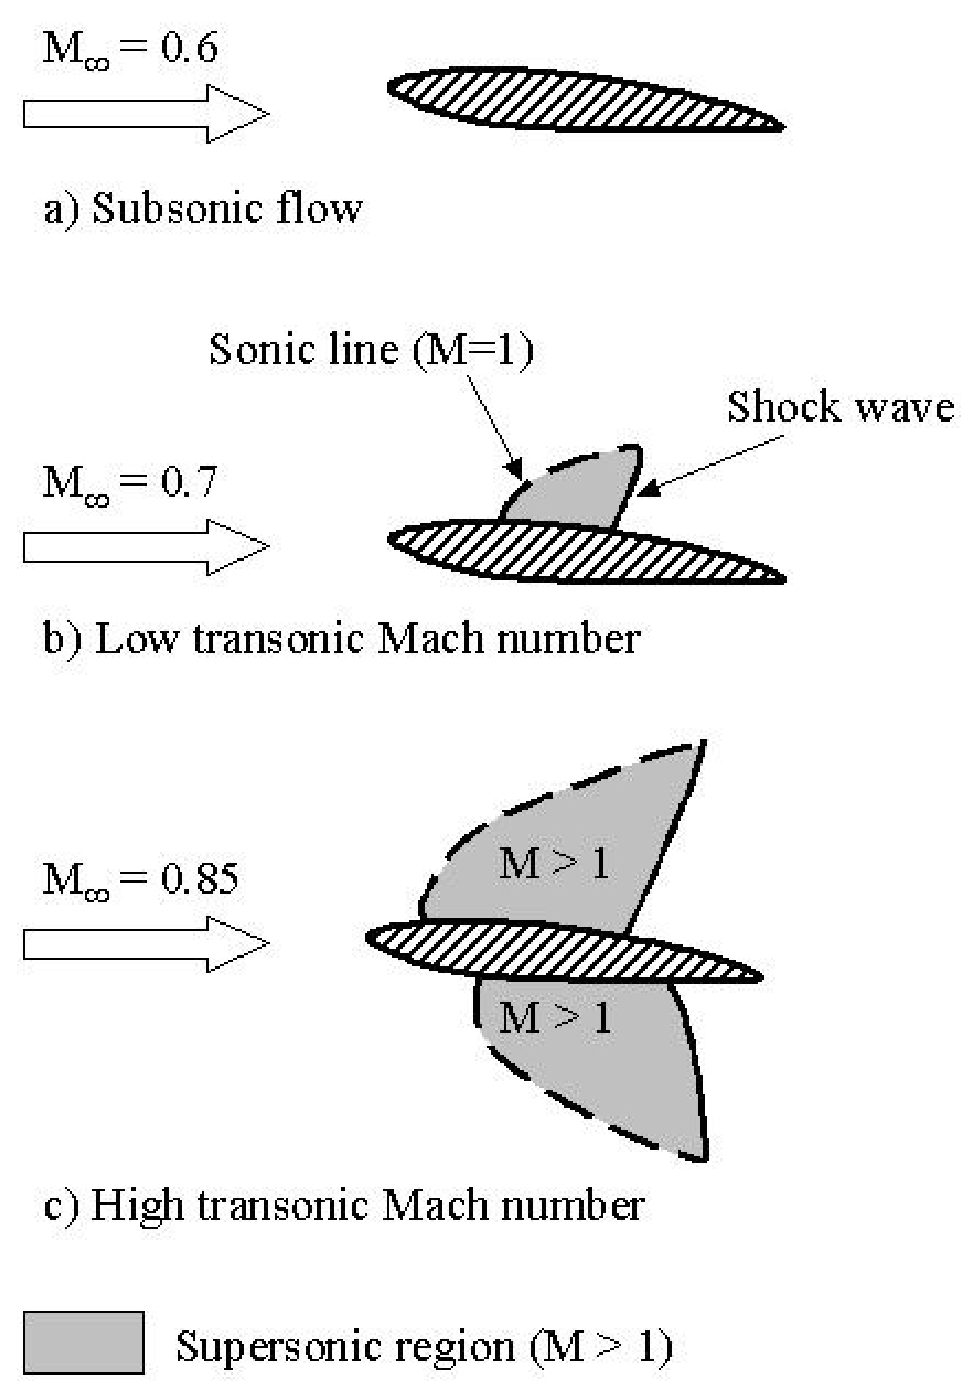
\includegraphics[height=6in]{aflow}
    \else
      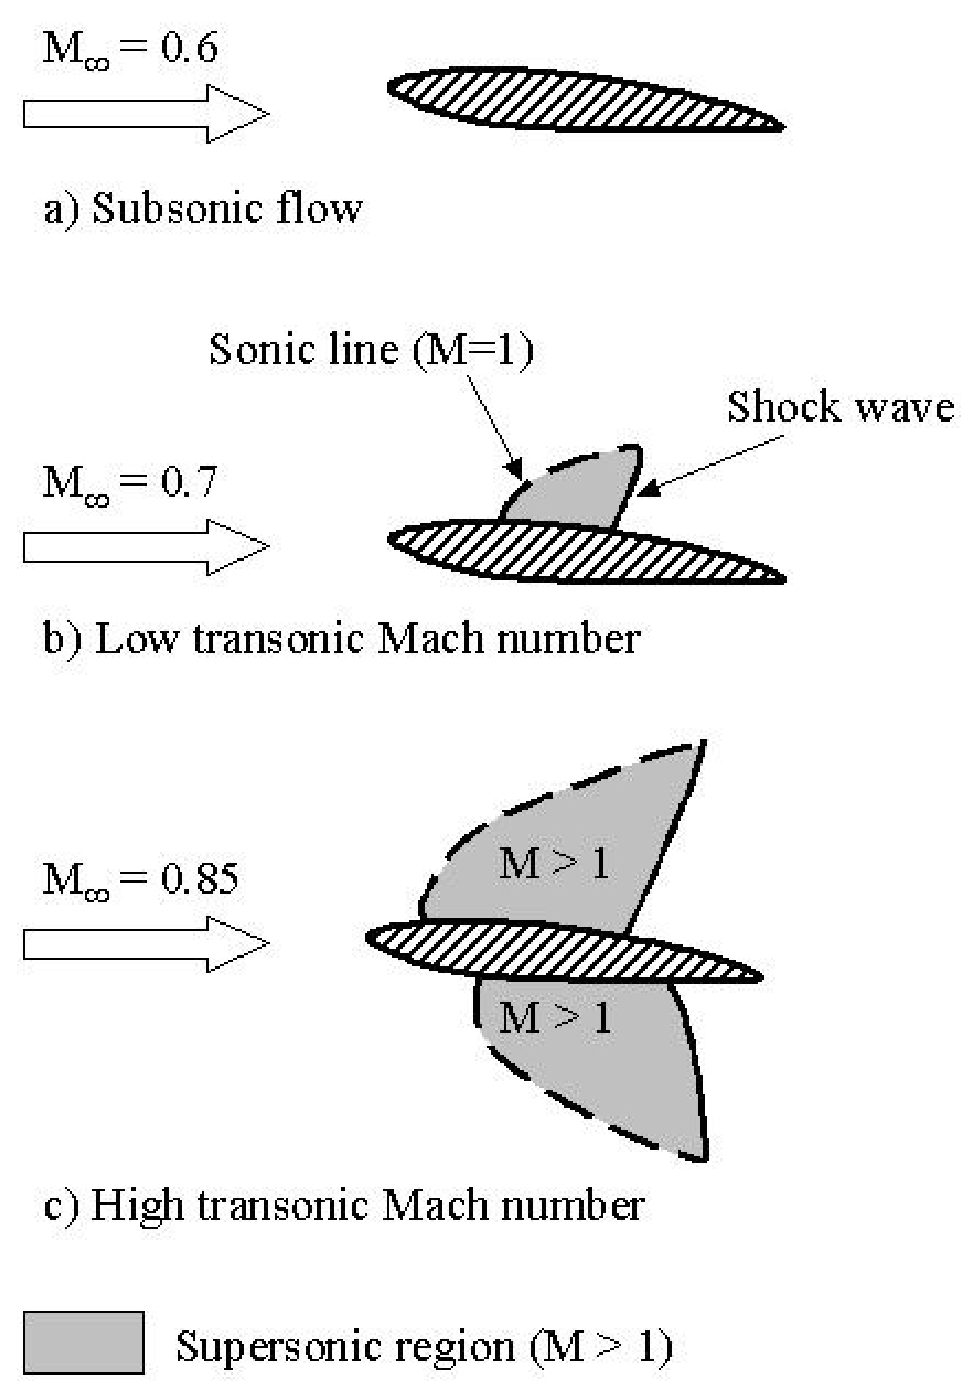
\includegraphics[bb = 92 86 545 742, height=6in]{aflow}
    \fi
    \caption{Airfoil Picture}
    \label{FigAir}
  \end{center}
\end{figure}

% above code has been macro-fied in Classes/MacroFile.tex file
%\InsertFig{\IncludeGraphicsH{aflow}{6in}{92 86 545 742}}{Airfoil Picture}{FigAir}

So as we have now labelled it we can reference it, like so Figure~(\ref{FigAir}) and it
is on Page \pageref{FigAir}. And as we can see, it is a very nice picture and we
can talk about it all we want and when we are tired we can move on to the next
chapter ...

I would also like to add an extra bookmark in acroread like so ...
\ifpdf
  \pdfbookmark[2]{bookmark text is here}{And this is what I want bookmarked}
\fi
\end{comment}
% ------------------------------------------------------------------------


%%% Local Variables: 
%%% mode: latex
%%% TeX-master: "../thesis"
%%% End: 

\chapter{Deterministic Model of Reproduction and Selection}
\ifpdf
    \graphicspath{{DeterministicModelofReproductionandSelection/Chapter2Figs/PNG/}{DeterministicModelofReproductionandSelection/Chapter2Figs/PDF/}{DeterministicModelofReproductionandSelection/Chapter2Figs/}}
\else
    \graphicspath{{DeterministicModelofReproductionandSelection/Chapter2Figs/EPS/}{DeterministicModelofReproductionandSelection/Chapter2Figs/}}
\fi
By determinism we means that given some conditions the final result is always  the same. For example if you know the initial frequencies and the rates of birth and death of two interacting species and measure  the frequencies at a certain time, this process is deterministic if every time  you set the same initial frequencies, you get the same final conditions at the same times. Deterministic population growth models are useful from understanding  the dynamic processes of growing and in predicting population frequencies and steady states. These deterministic models are divided in two types: discrete and continuos. This chapter gives some basic concepts of these two types that will be used for the development of this work. Furthermore in the last part of this chapter a continuos model of natural selection will be explained. 
\section{Discrete Model}
In discrete models of population growth the number $N$ of individuals increases with each time step $\Delta t$. The population at time $t+\tau$ is a recurrence function of the present generation at time $t$ and past populations, 
\begin{equation}
N_{t+\Delta t}=f(N_{t},N_{t-\Delta t}, ......, N_{0}),
\end{equation}
but usually it is just a function of the present population
\begin{equation}
N_{t+\Delta t}=f(N_{t}).
\end{equation} 
Given the initial conditions, the recurrence relation is solved if  it is possible to write $N_{n\Delta t }$ in terms of the initial conditions, $n$ and $\Delta t$. This allows us to know the state of the $n$ generation without using the recursion equation. 

Most of the recurrence relations have no solution, but even then, they  allow us to know about the properties of population dynamics, such as the existence of steady states. Due to this fact, they are essential for the algorithms in computational simulations of biological systems, as for example, the Fibonacci sequence for modeling rabbit population growth and plant patterning.

  
Now one of the most popular examples of discrete processes in literature will be shown. Suppose that at certain average period of time an individual divides; for example consider a cell and its offsprings that divide into  $r$ cells each time $\tau$. The  equation of this process is
\begin{equation}
N_{t+\tau}=rN_{t},
\end{equation} 
this is a recurrence equation, and the solution in terms of the initial condition $x_{0}$ after $n$ periods of time is
\begin{equation}
N_{n\tau}=N_{0}r^{n\tau}.
\end{equation}
The recurrence relation can be transformed to 
\begin{equation}
N_{t+\tau}-N_{t}=(r-1)N_{t},
\end{equation}
that is a difference equation of first order. 
For long times and taking $\tau=1$, this discrete equation can be transformed into a differential equation in time. 
\section{Continuous Model}
%Continuous model are good for population dynamics after times much larger than the time step of reproduction.
The most simple system in continuous growth is the single species model of birth. Where the per capita rate of change in population is due to the reproductive contribution $r$ of each individual,
\begin{equation}
\frac{dN(t)}{dt}=rN(t),
\end{equation} 
but this is for growth in a perfect environment. In a more realistic situation, without considering ecological interactions, there are death rate $d$ and migration $m$. Then the rate of change in the population would be 
\begin{equation}
\frac{dN(t)}{dt}=rN(t)-dN(t)-mN(t).
\end{equation}
 The solution of this equation is
 \begin{equation}
 N(t)=N_{0}e^{(r-d-m)t},
 \end{equation}
 where if $r-d-m$ is positive the population will growth and if $r-d-m$ it will decrease.
 
 Now let us see a continuous model of natural selection, where we have a population of constant size $N$ and two or more species competing. The constant size condition will generate selection and in a realistic situation it can be set up to maintain the population  at its maximum carrier capacity.
 
 Suppose we have two organisms $A$ and $B$ competing, with fitnesses $f_{A}$ and $f_{B}$ and frequencies $x_A$ and $x_B$ respectively. Because of the constant size $x_A+x_B=N$, there is a rate of death $\phi$ common to the two populations of organisms that keeps this condition. The differential equations for these two types are
 \begin{equation}
 \frac{dx_A}{dt} =f_A x_{A} - \phi,
 \end{equation}  
  \begin{equation}
 \frac{dx_B}{dt} =f_B x_{B} - \phi.
 \end{equation}  
 Solving these two equations for $\phi$
 \begin{equation}
 \phi = \frac{x_{A}f_{A}+x_{B}f_{B}}{N},
 \end{equation}
 and replacing $\phi$ in the equation for $x_{A}$, we obtain the differential equation for it
 \begin{equation}\label{3.12}
\frac{dx_{A}}{dt}=x_{A}(1-\frac{x_{A}}{N})(f_{A}-f_{B}).
 \end{equation} 
Its solution is 
\begin{equation}
x_{A}(t)=\frac{x_{A0}e^{(f_{A}-f_{B})t}}{1-\frac{x_{A0}}{N}+\frac{x_{A0}}{N}e^{(f_{A}-f_{B})t}}.
\end{equation}  
In these two equations it can be seen that the dominance of $A$ depends only on the fact that its fitness is larger than the fitness of $B$  (Figure \ref{Fig3.1}), and the time of fixation will be shorter if the initial population increases Figure (3.2). It can be seen also that the equilibrium points are the points of dominance. 
\begin{figure}[H]
  \begin{center}
    \leavevmode
    \ifpdf
      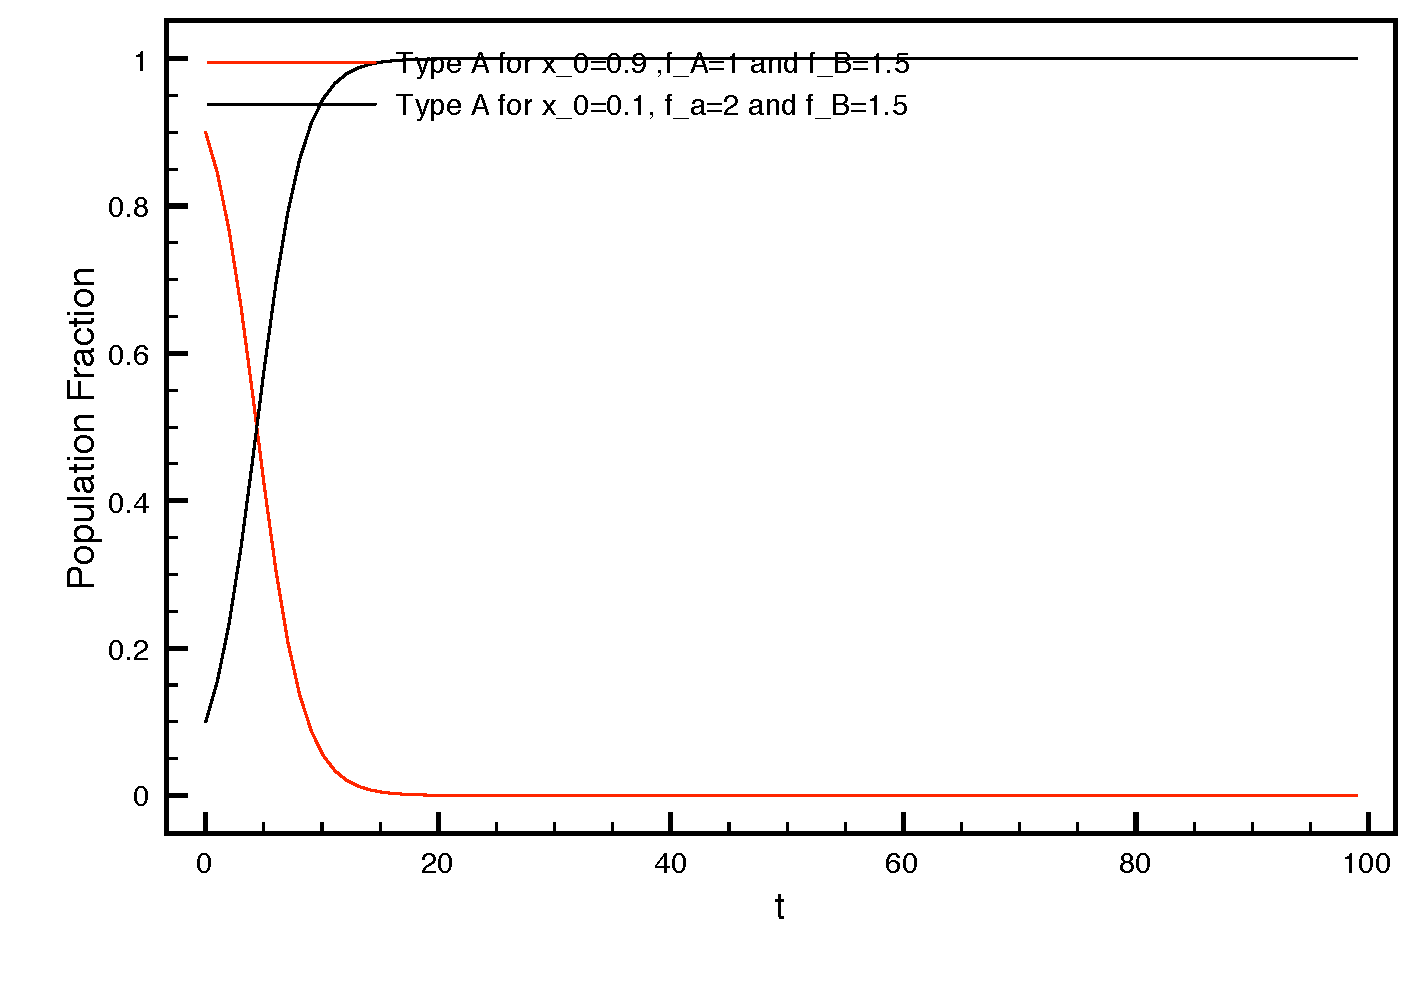
\includegraphics[width=7cm,height=7cm]{DeterministicSelection.pdf}
    \else
      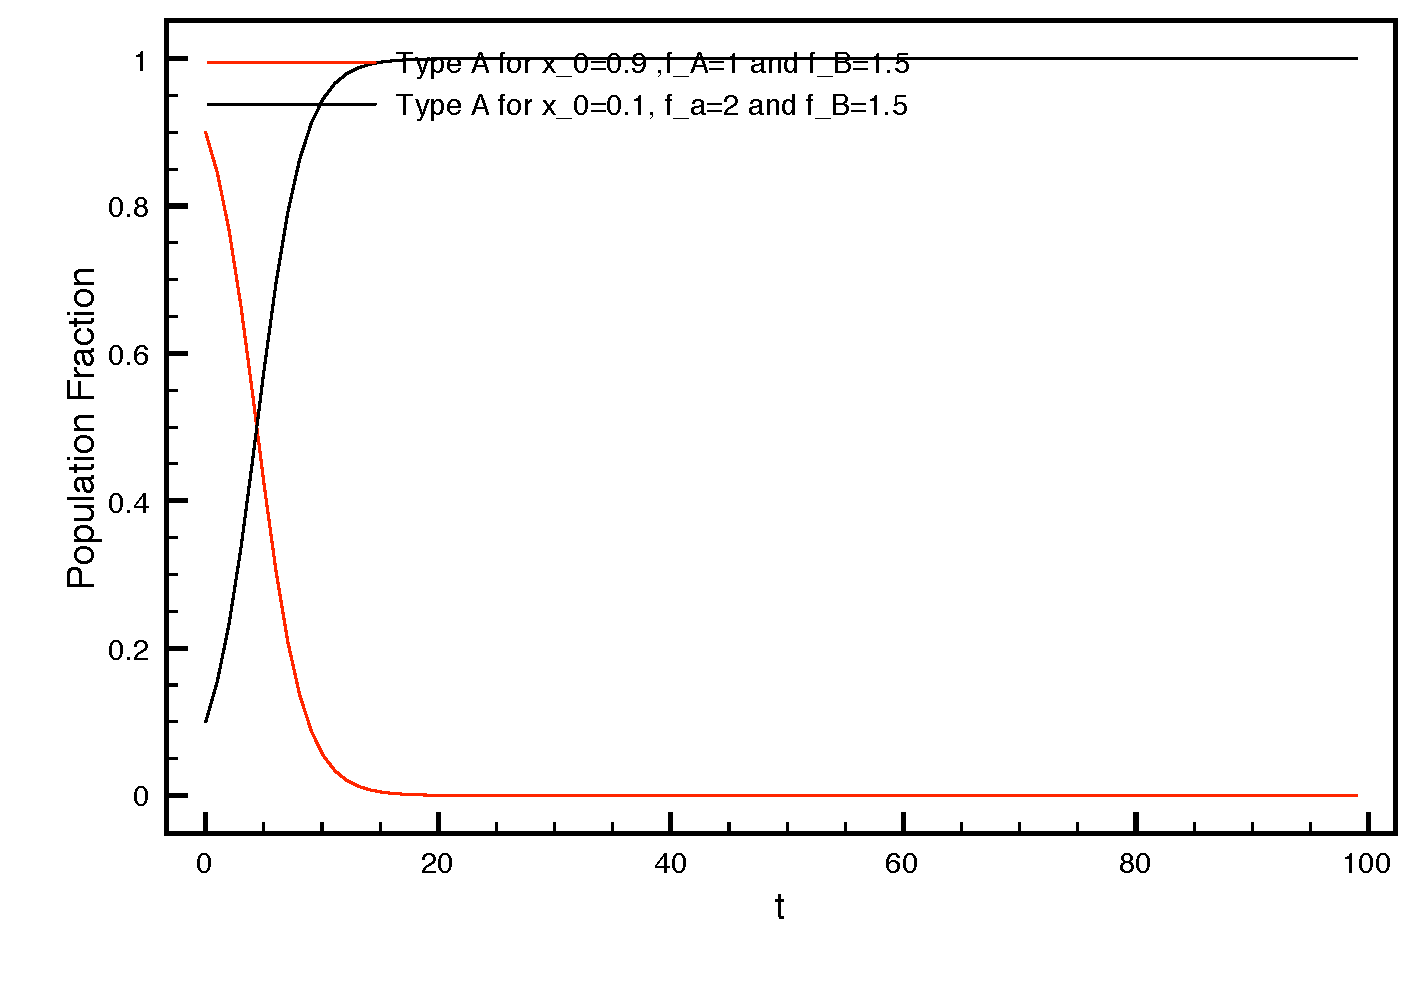
\includegraphics[width=7cm, height=7cm]{DeterministicSelection.pdf}
    \fi
    \caption{Fraction of $x_{A}$ for two different conditions of initial population and fitness.}
    \label{Fig3.1}
  \end{center}
  \end{figure}
  
\begin{figure}[H]
  \begin{center}
    \leavevmode
    \ifpdf
      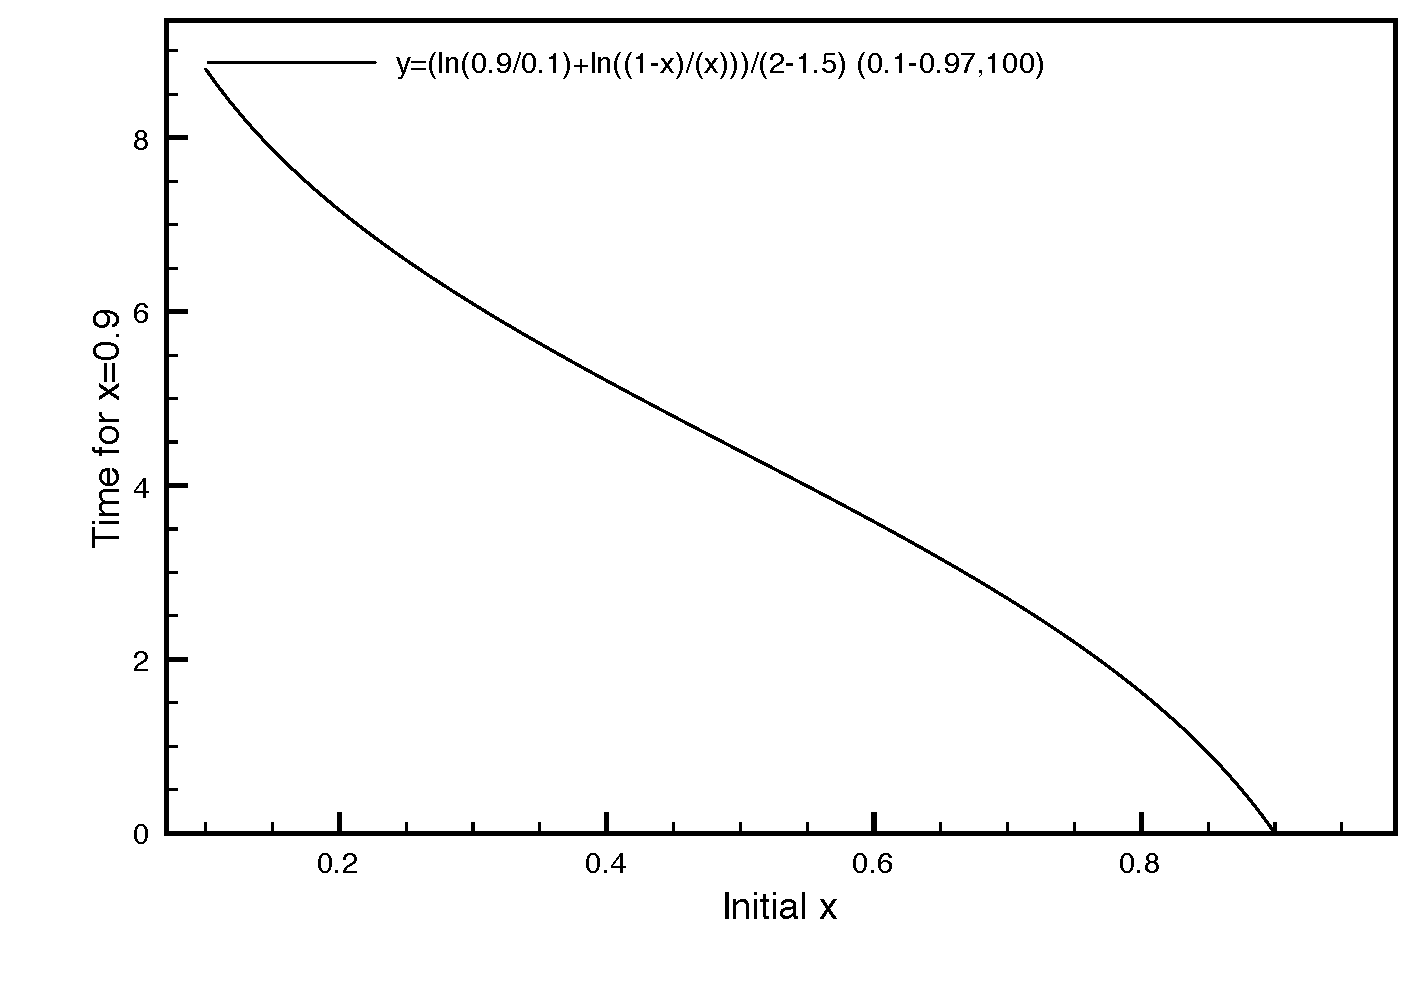
\includegraphics[width=7cm,height=7cm]{DominanceTimeVsInitialx.pdf}
    \else
      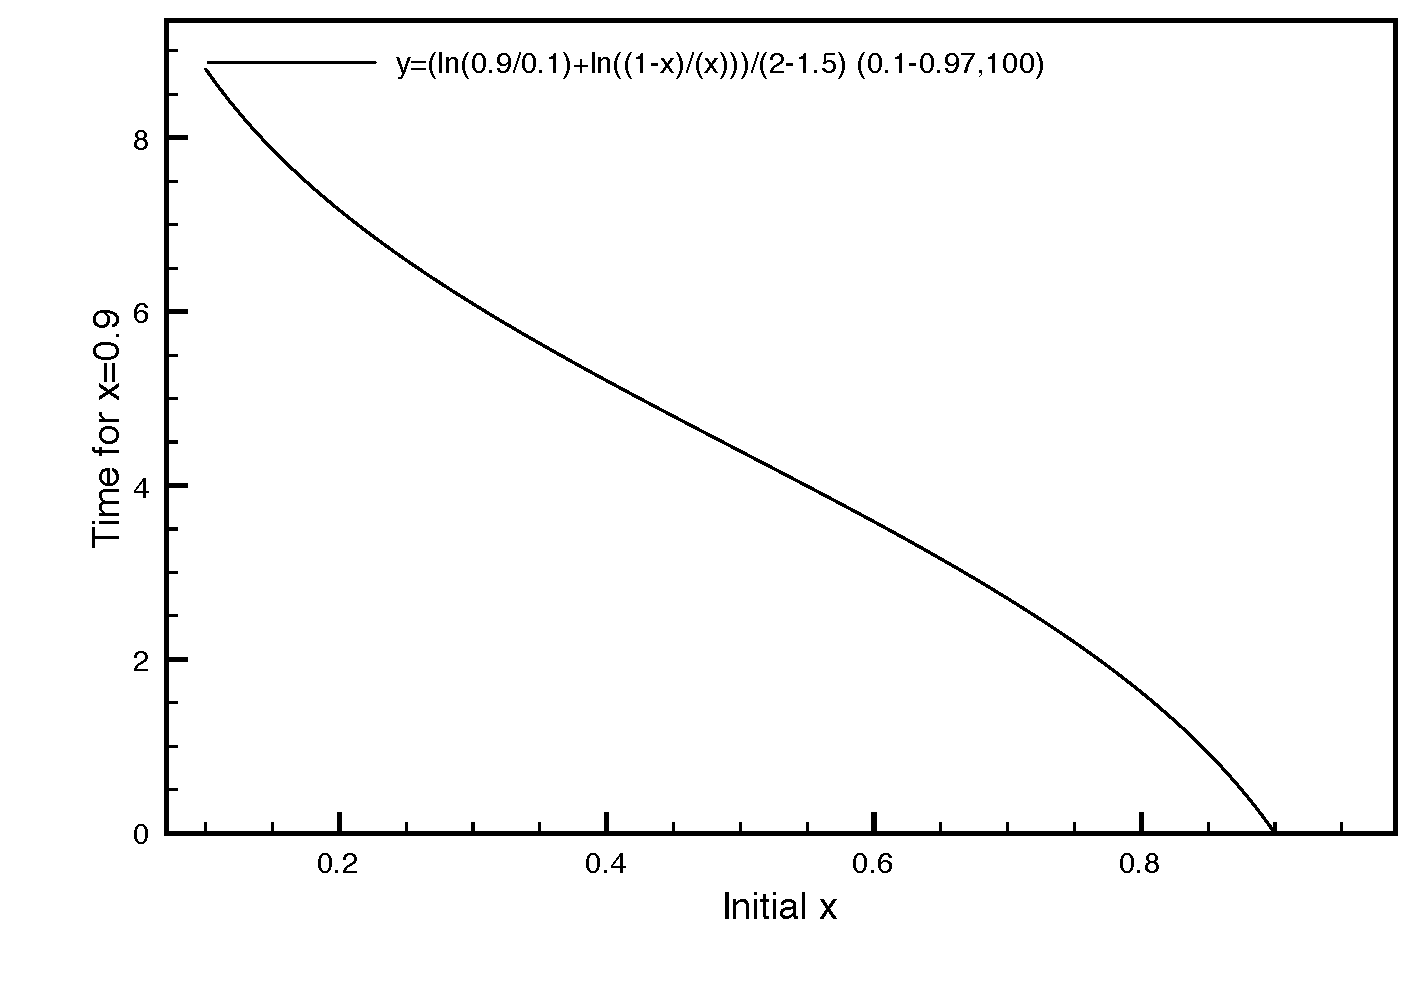
\includegraphics[width=7cm, height=7cm]{DominanceTimeVsInitialx.pdf}
    \fi
    \caption{Time when $x_{A}$ reach the $0.9$ fraction of population as a function of the initial $x_{A}$.}
    \label{FigAir2}
  \end{center}
\end{figure}

The problem with this model is that it does not let us  see the intrinsic process of selection, how each individual is chosen over the others for reproduction and finally a type invades the population. Later we will see the stochastic model for a situation of constant size and two types with different fitness.  
% ------------------------------------------------------------------------

%%% Local Variables: 
%%% mode: latex
%%% TeX-master: "../thesis"
%%% End: 

\renewcommand{\chaptername}{}
\chapter{Markov Chain }
\ifpdf
    \graphicspath{{MarkovChain/Chapter3Figs/PNG/}{MarkovChain/Chapter3Figs/PDF/}{MarkovChain/Chapter3Figs/}}
\else
    \graphicspath{{MarkovChain/Chapter3Figs/EPS/}{MarkovChain/Chapter3Figs/}}
\fi
\markboth{\MakeUppercase{\thechapter. Markov Chain}}{\thechapter. Markov Chain}
In this part, some properties of stochastic processes and the approach of a Markov chain to calculate the probabilities of the absorbing states  and absorbance times in such systems will be explained. Competition and natural selection in biological scenarios, which are modeled with Moran process, have the properties of such stochastic systems. This relation allows us to calculate analytically expressions for fixation probability and average time of fixation of a new mutant or group of mutants competing with the old population in two cases: random and neutral drift.  
  
 

\section{ Moran process}
This process is a stochastic model that was created by Moran to simulate selection among different types of individuals across generations in finite populations, where the organism with the largest fitness will invade the whole population depending on the initial population.   


Imagine an experiment where a population of bacteria is at its maximal carrier capacity; then the population size will be constant, and that means that when an offspring is born other individual has to die. 
This is the Moran process, where at each time step one individual of the population is chosen randomly for reproduction with a probability that depends of its fitness. In order to keep a constant population size, the new offspring replaces another individual of the population that is chosen randomly as is depicted in Figure (\ref{Fig41}). 

\begin{figure}[H]
  \begin{center}
    \leavevmode
    \ifpdf
      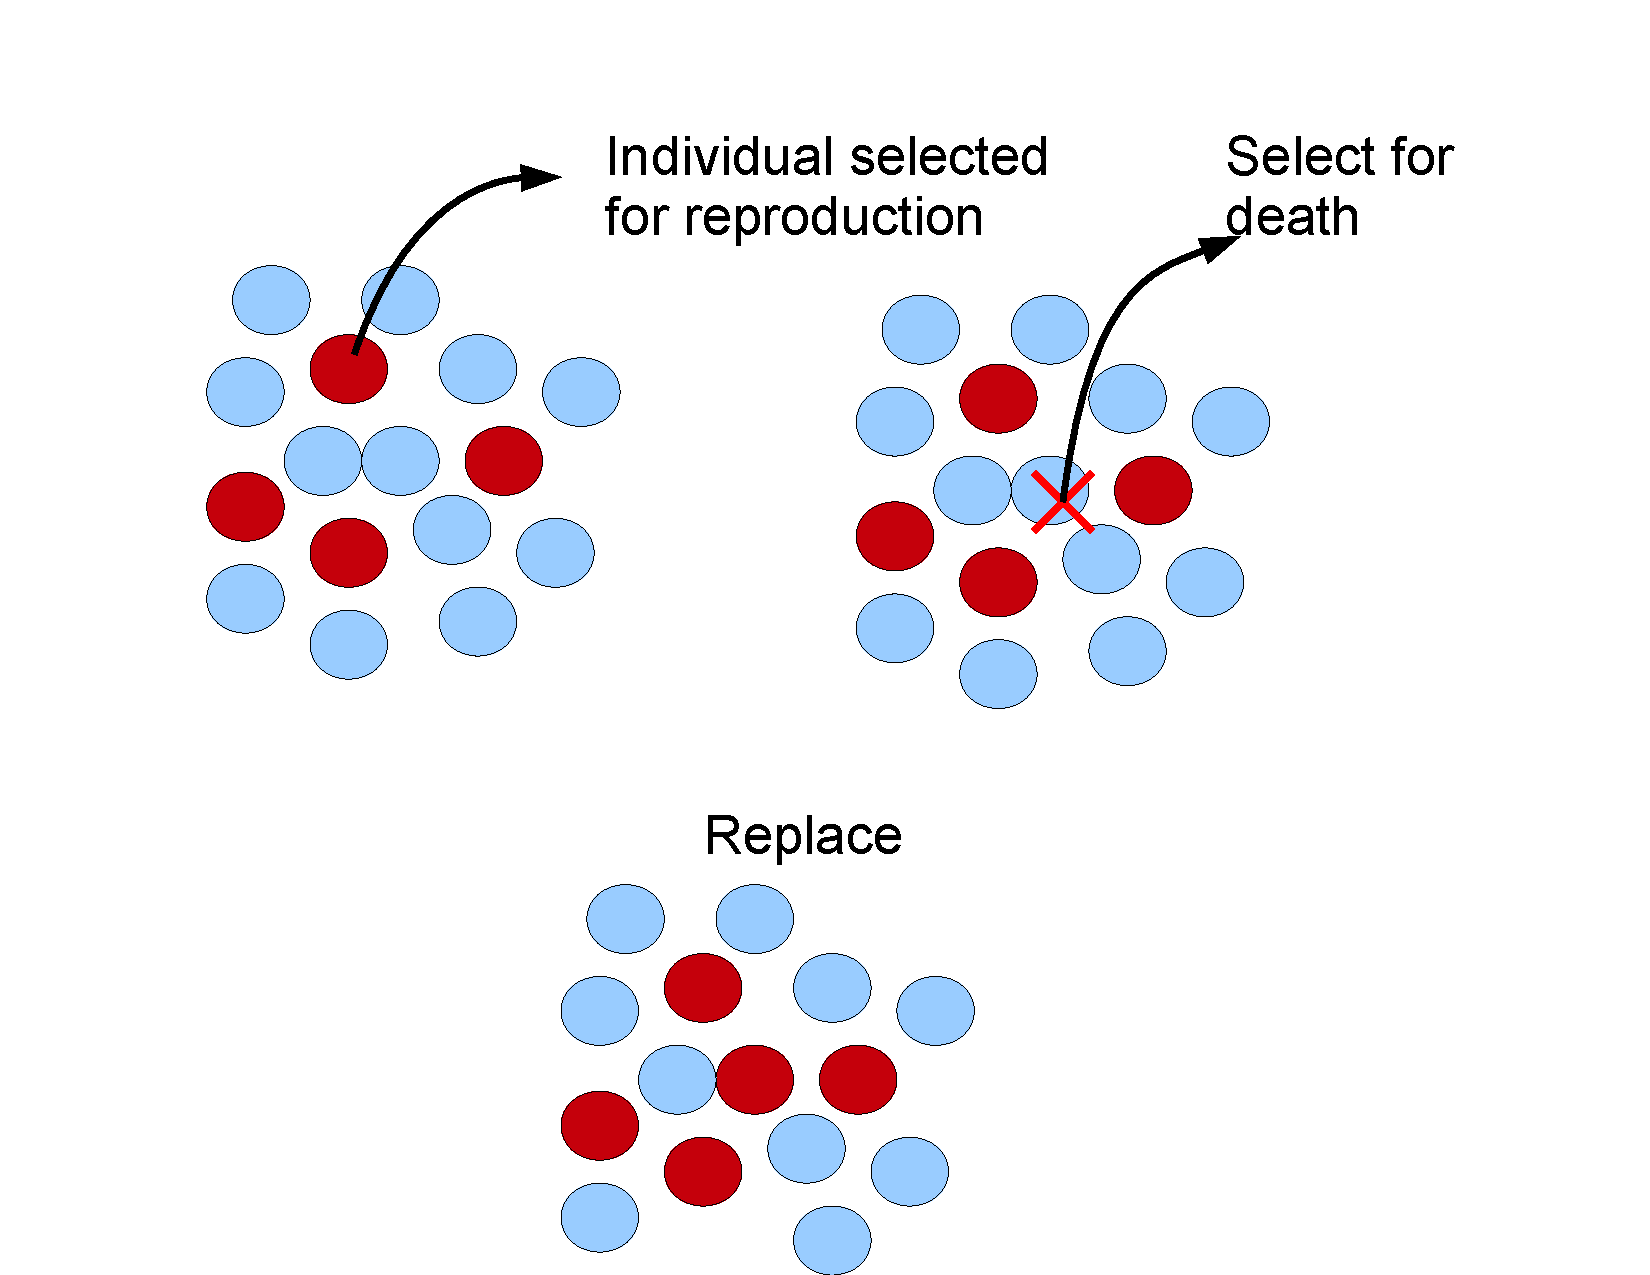
\includegraphics[width=7cm,height=5cm]{moranprocess.pdf}
    \else
      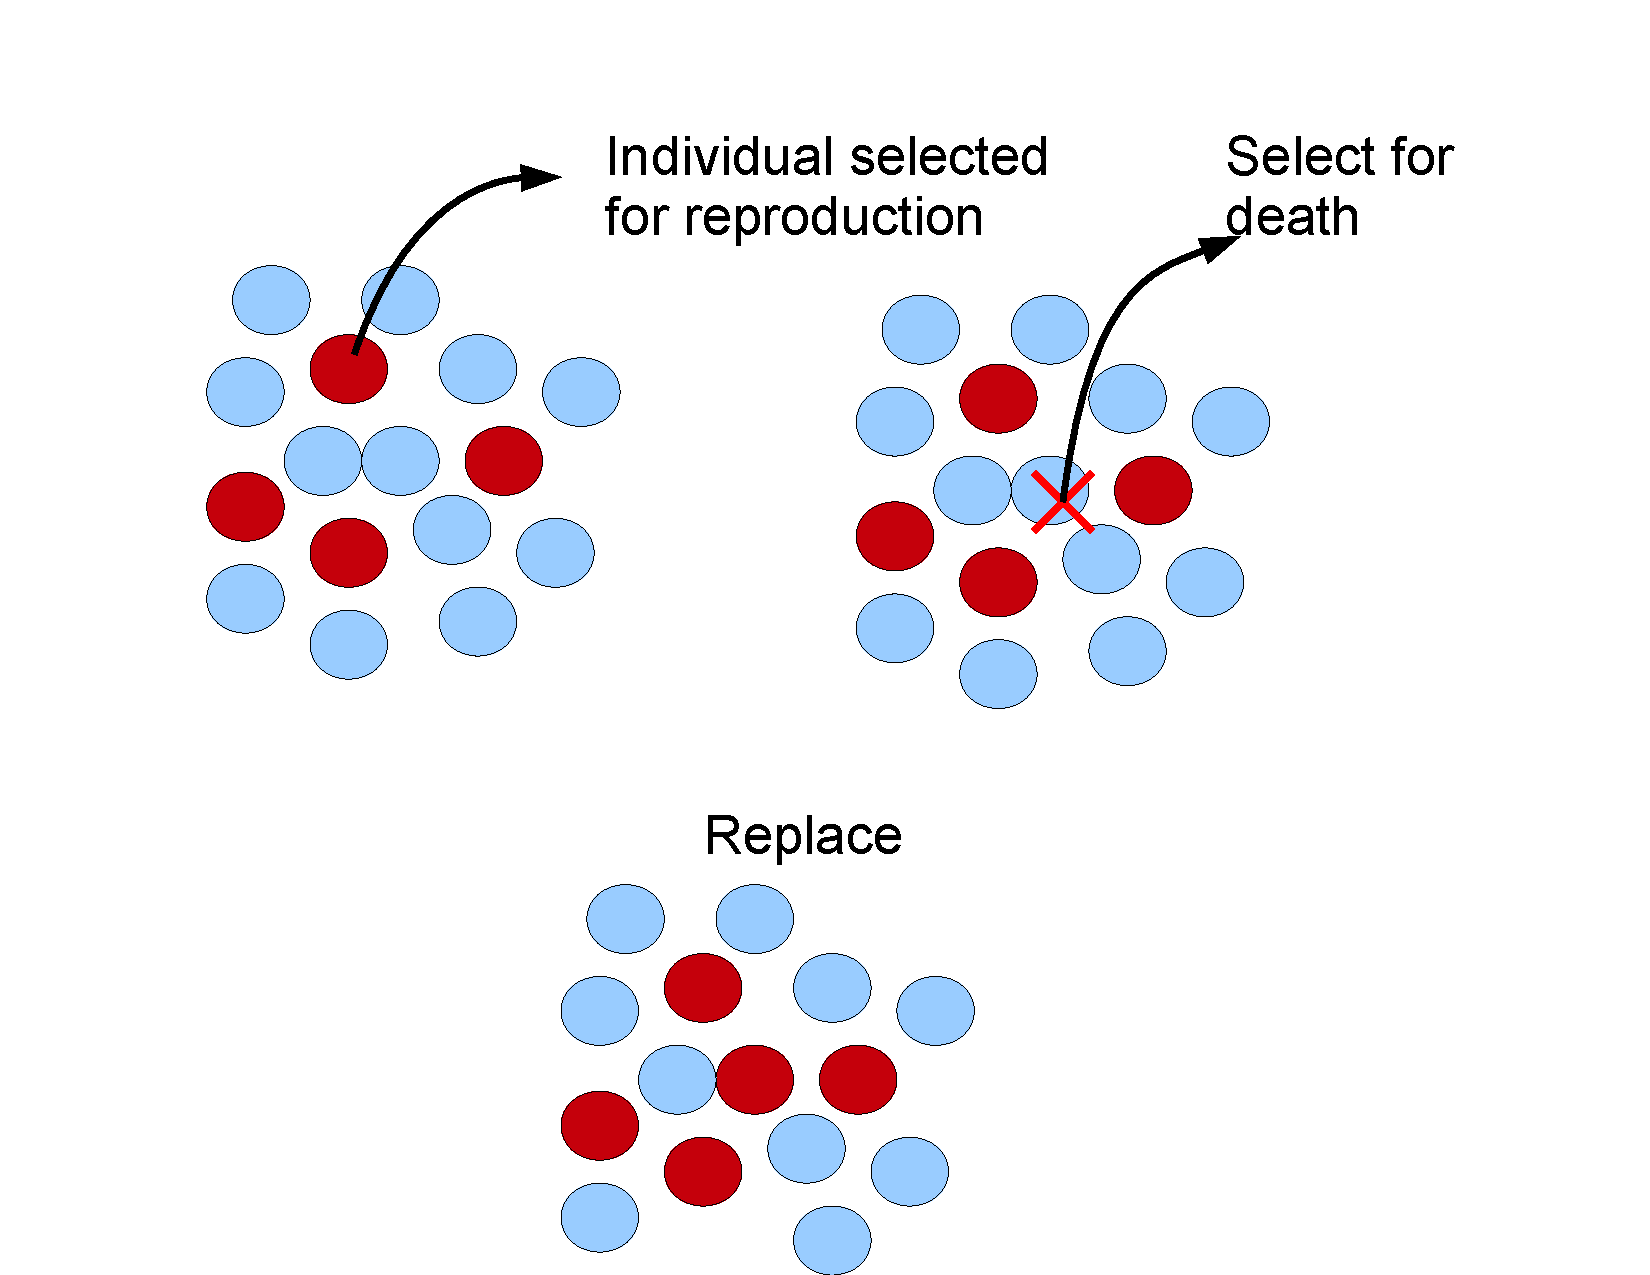
\includegraphics[width=7cm, height=5cm]{moranprocess.pdf}
    \fi
    \caption{Example of birth and death in Moran process, where it is seen that the size population is constant.}
    \label{Fig41}
  \end{center}
  \end{figure}

Because a Moran process is a birth and death process, it is a Markov chain which has two absorbing states in the case of two types competing.

What is a Markov chain? A Markov chain is a random process with a set of discrete and finite states. In this process, the transitions from one state to another occurs in discrete time steps, where the transition to the next state depends only on the present state and not on the preceding sequence of states, which is the Markov property.

The next Figure (\ref{Fig42})  is a graph that represents a Markov chain, 
\begin{figure}[H]
 \begin{center}
    \leavevmode
    \ifpdf
      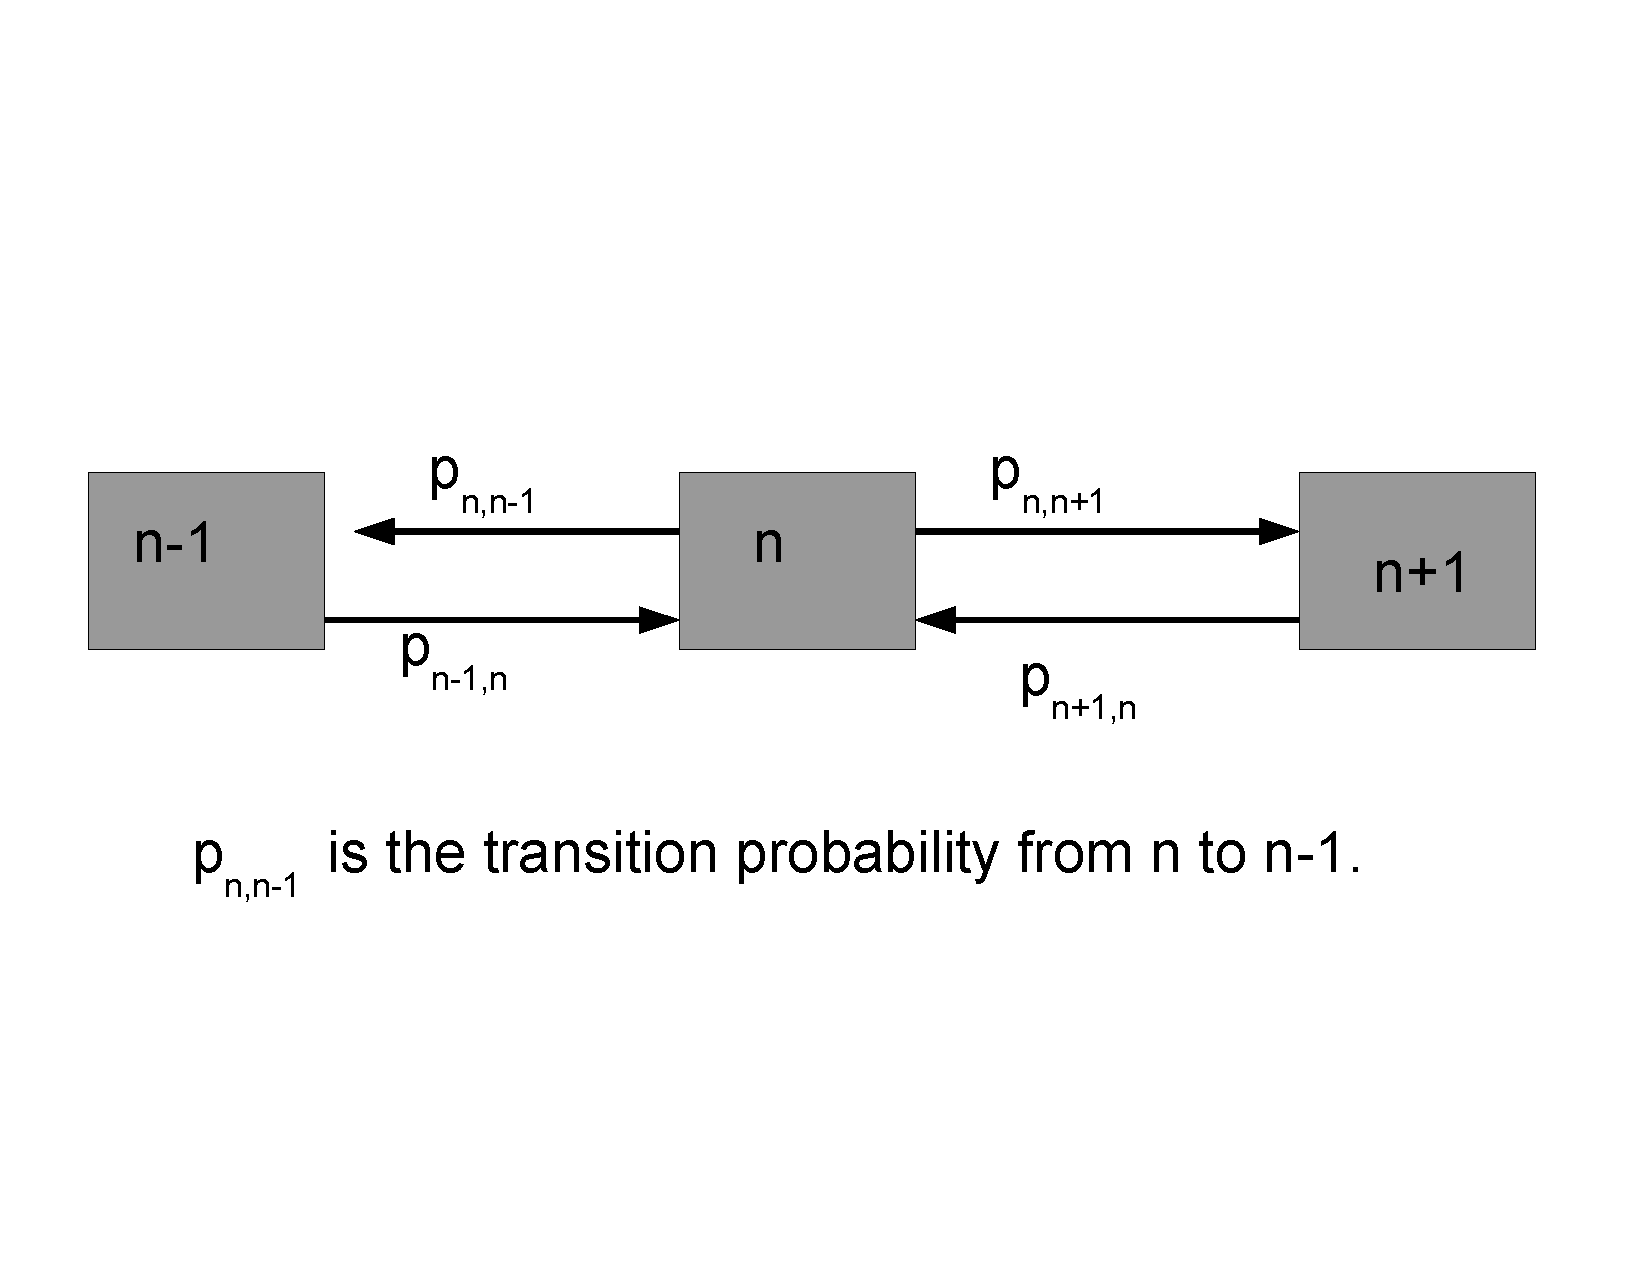
\includegraphics[width=7cm,height=5cm]{markovchain.pdf}
    \else
     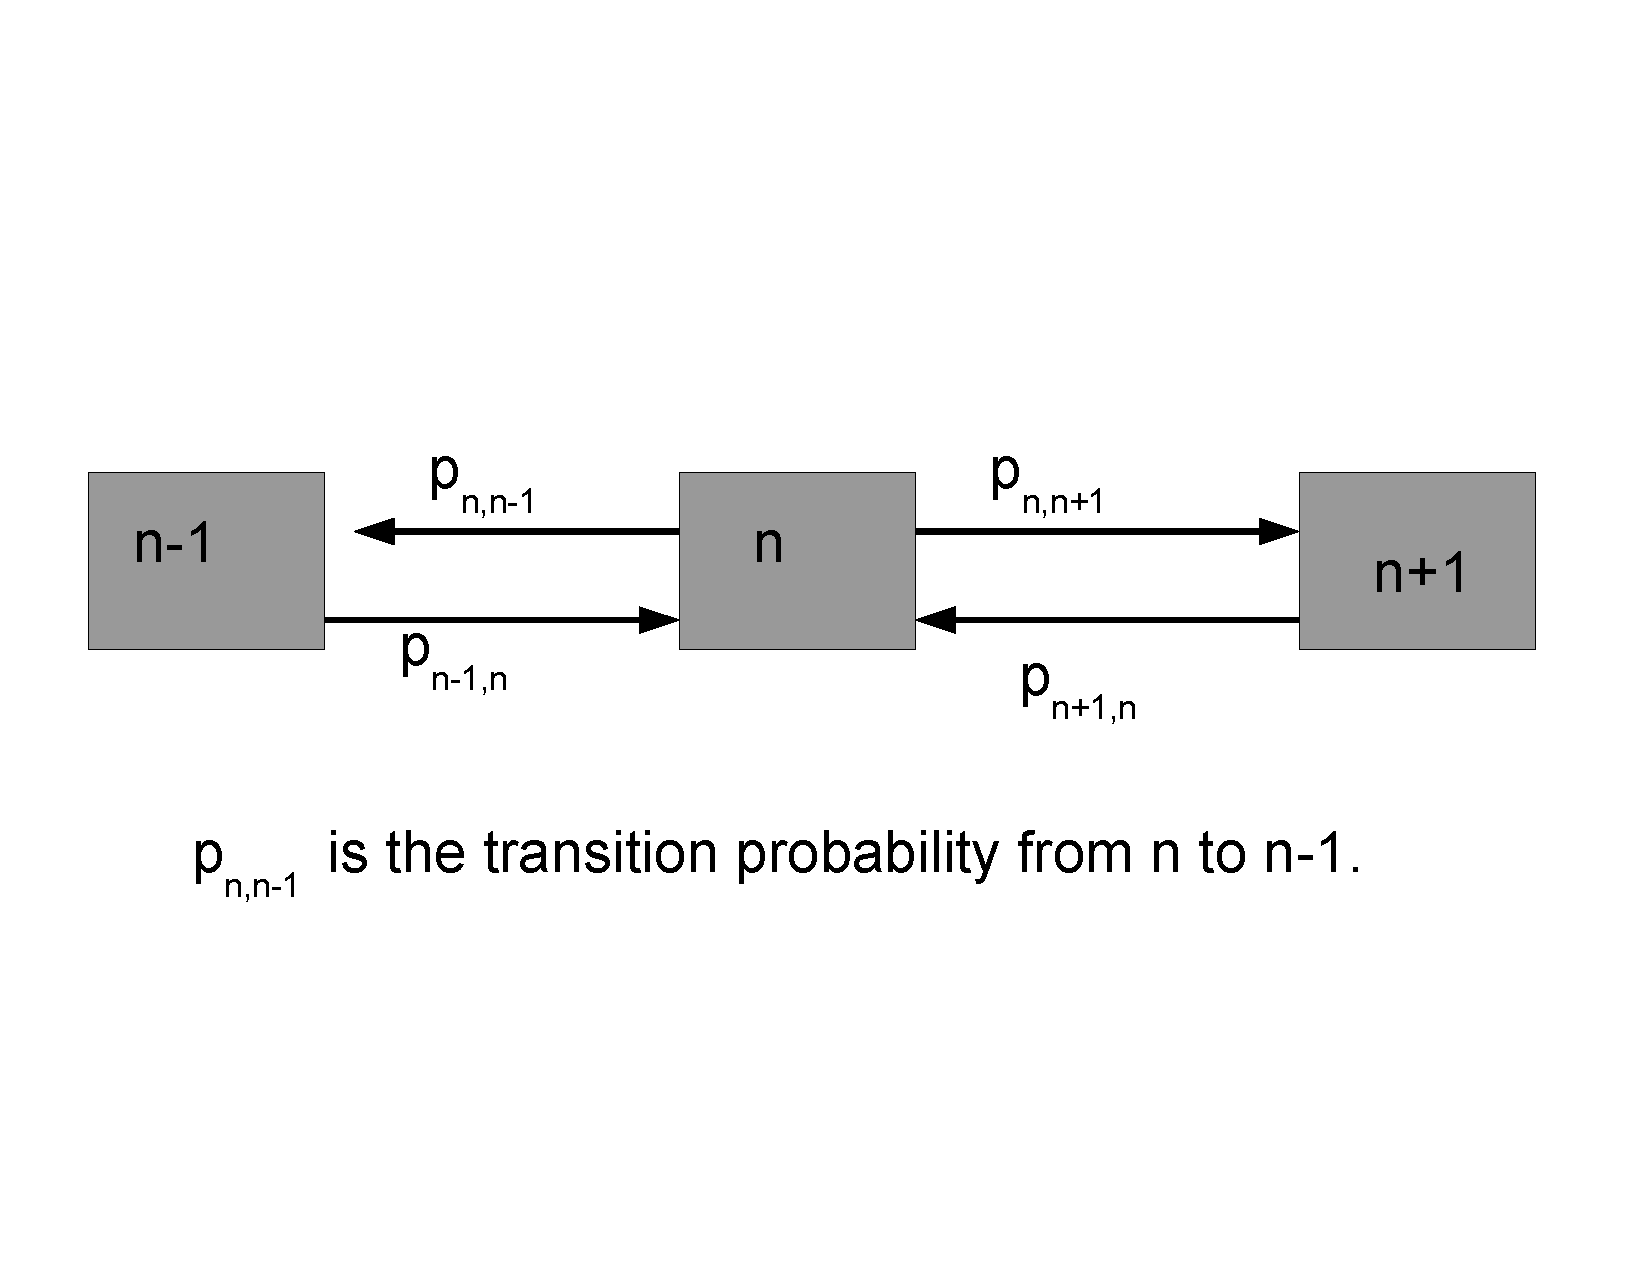
\includegraphics[width=7cm, height=5cm]{markovchain.pdf}
    \fi
    \caption{Graph of transitions in a Markov process.}
    
    \label{Fig42}
  \end{center}
  \end{figure}

where $n$, $n-1$ and $n+1$ are states of the system and the arrows represent the transition between neighbor states. The master equation for the probability flux of state $n$ is
\begin{equation}\label{4.1}
\frac{dP_{n}}{dt}=-(p_{n,n-1}+p_{n,n+1})P_{n}+p_{n-1,n}P_{n-1}+p_{n+1,n}P_{n+1}.
\end{equation} 
Now let us see the Markov graph representation for a simple Moran process in a population of size $N$ and two different organisms of type $A$ and $B$ Figure (\ref{Fig43}), where $n$ is the number of individuals of type $A$(red balls) and the system have a  population size $N=14$, the fitnesses for the two types are $f_{A}$ and $f_{B}$.
\begin{figure}[H]
 \begin{center}
    \leavevmode
    \ifpdf
      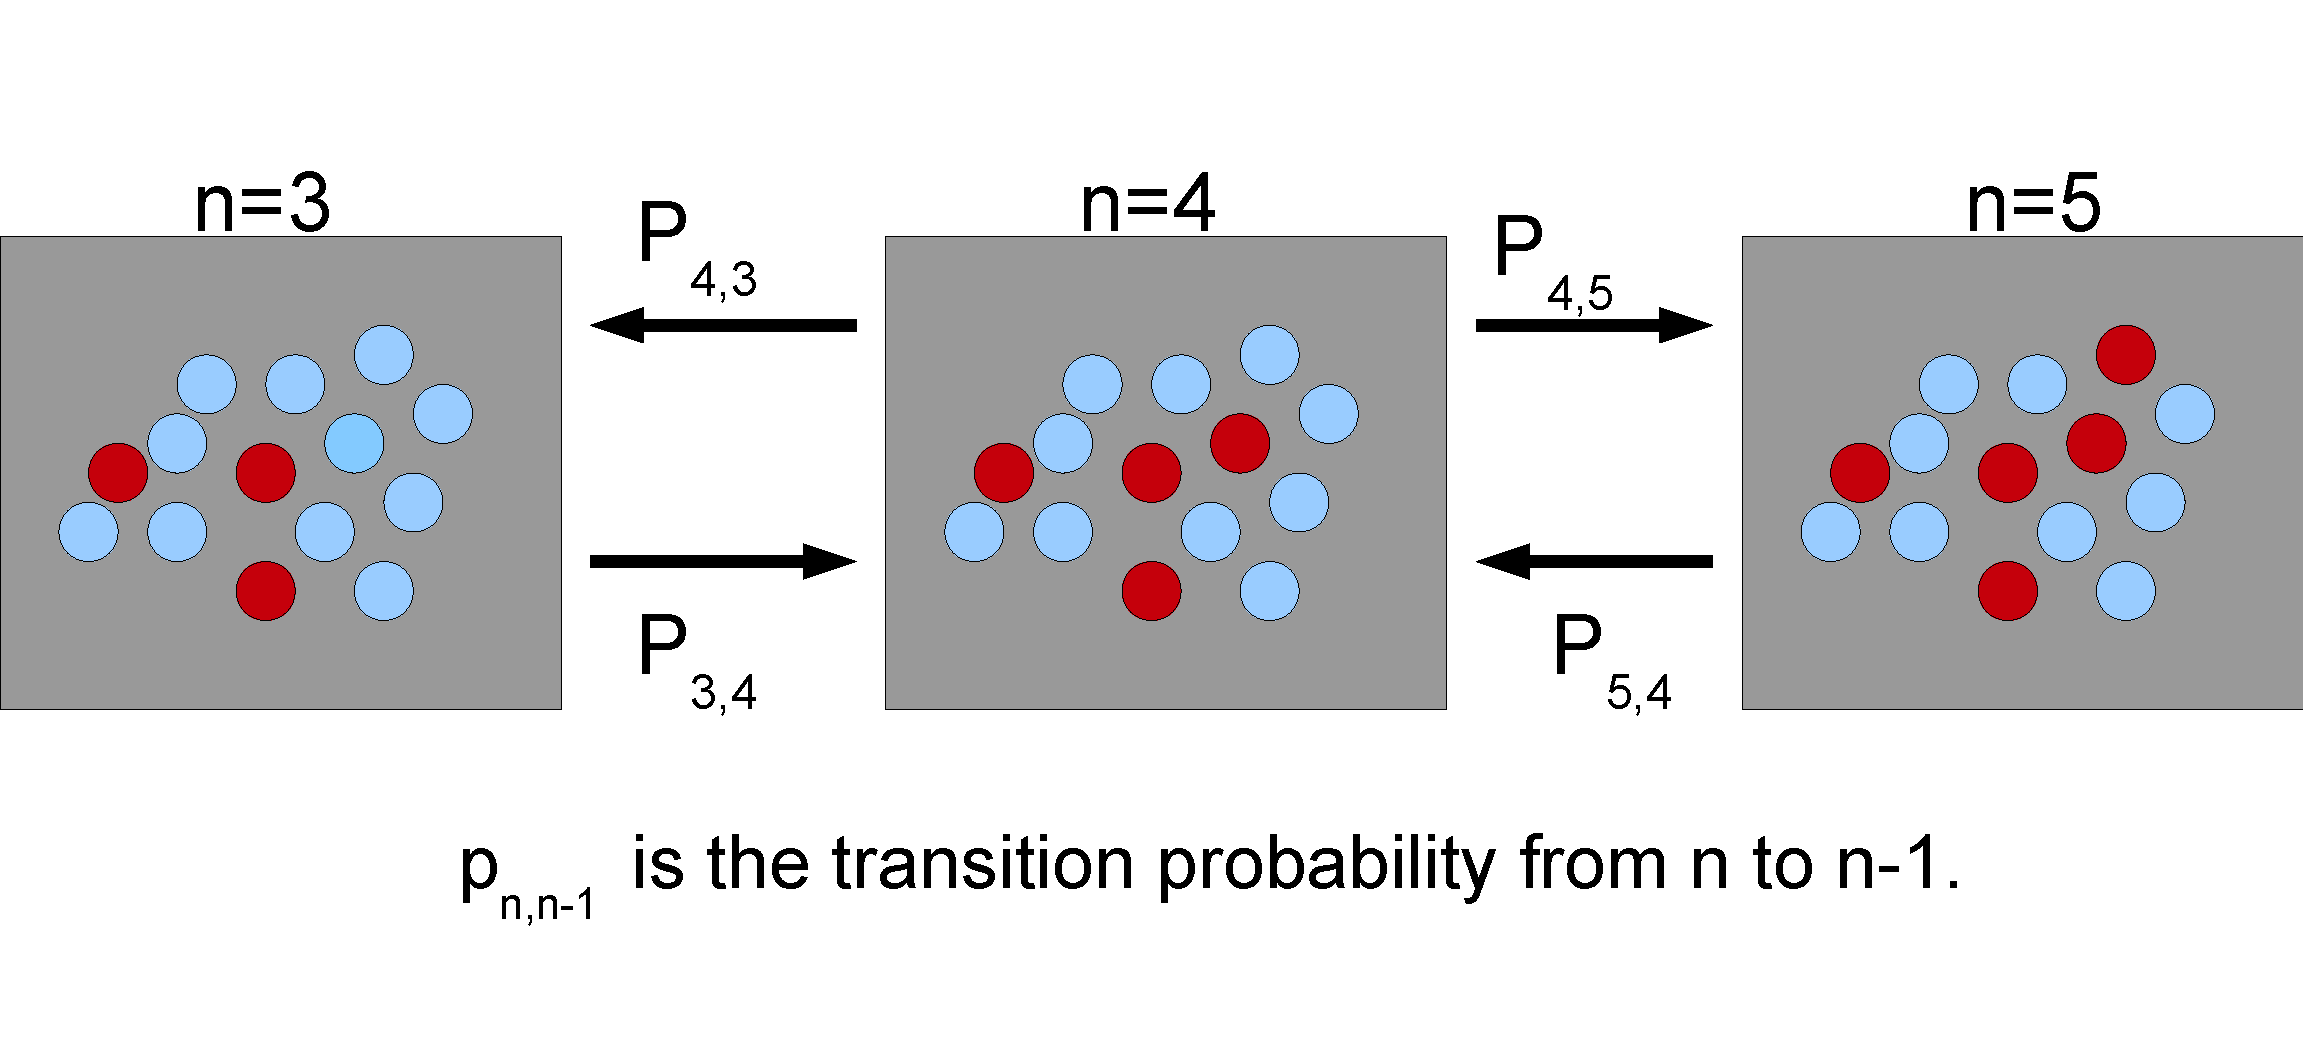
\includegraphics[width=9cm,height=7cm]{markovchainMoran.pdf}
    \else
     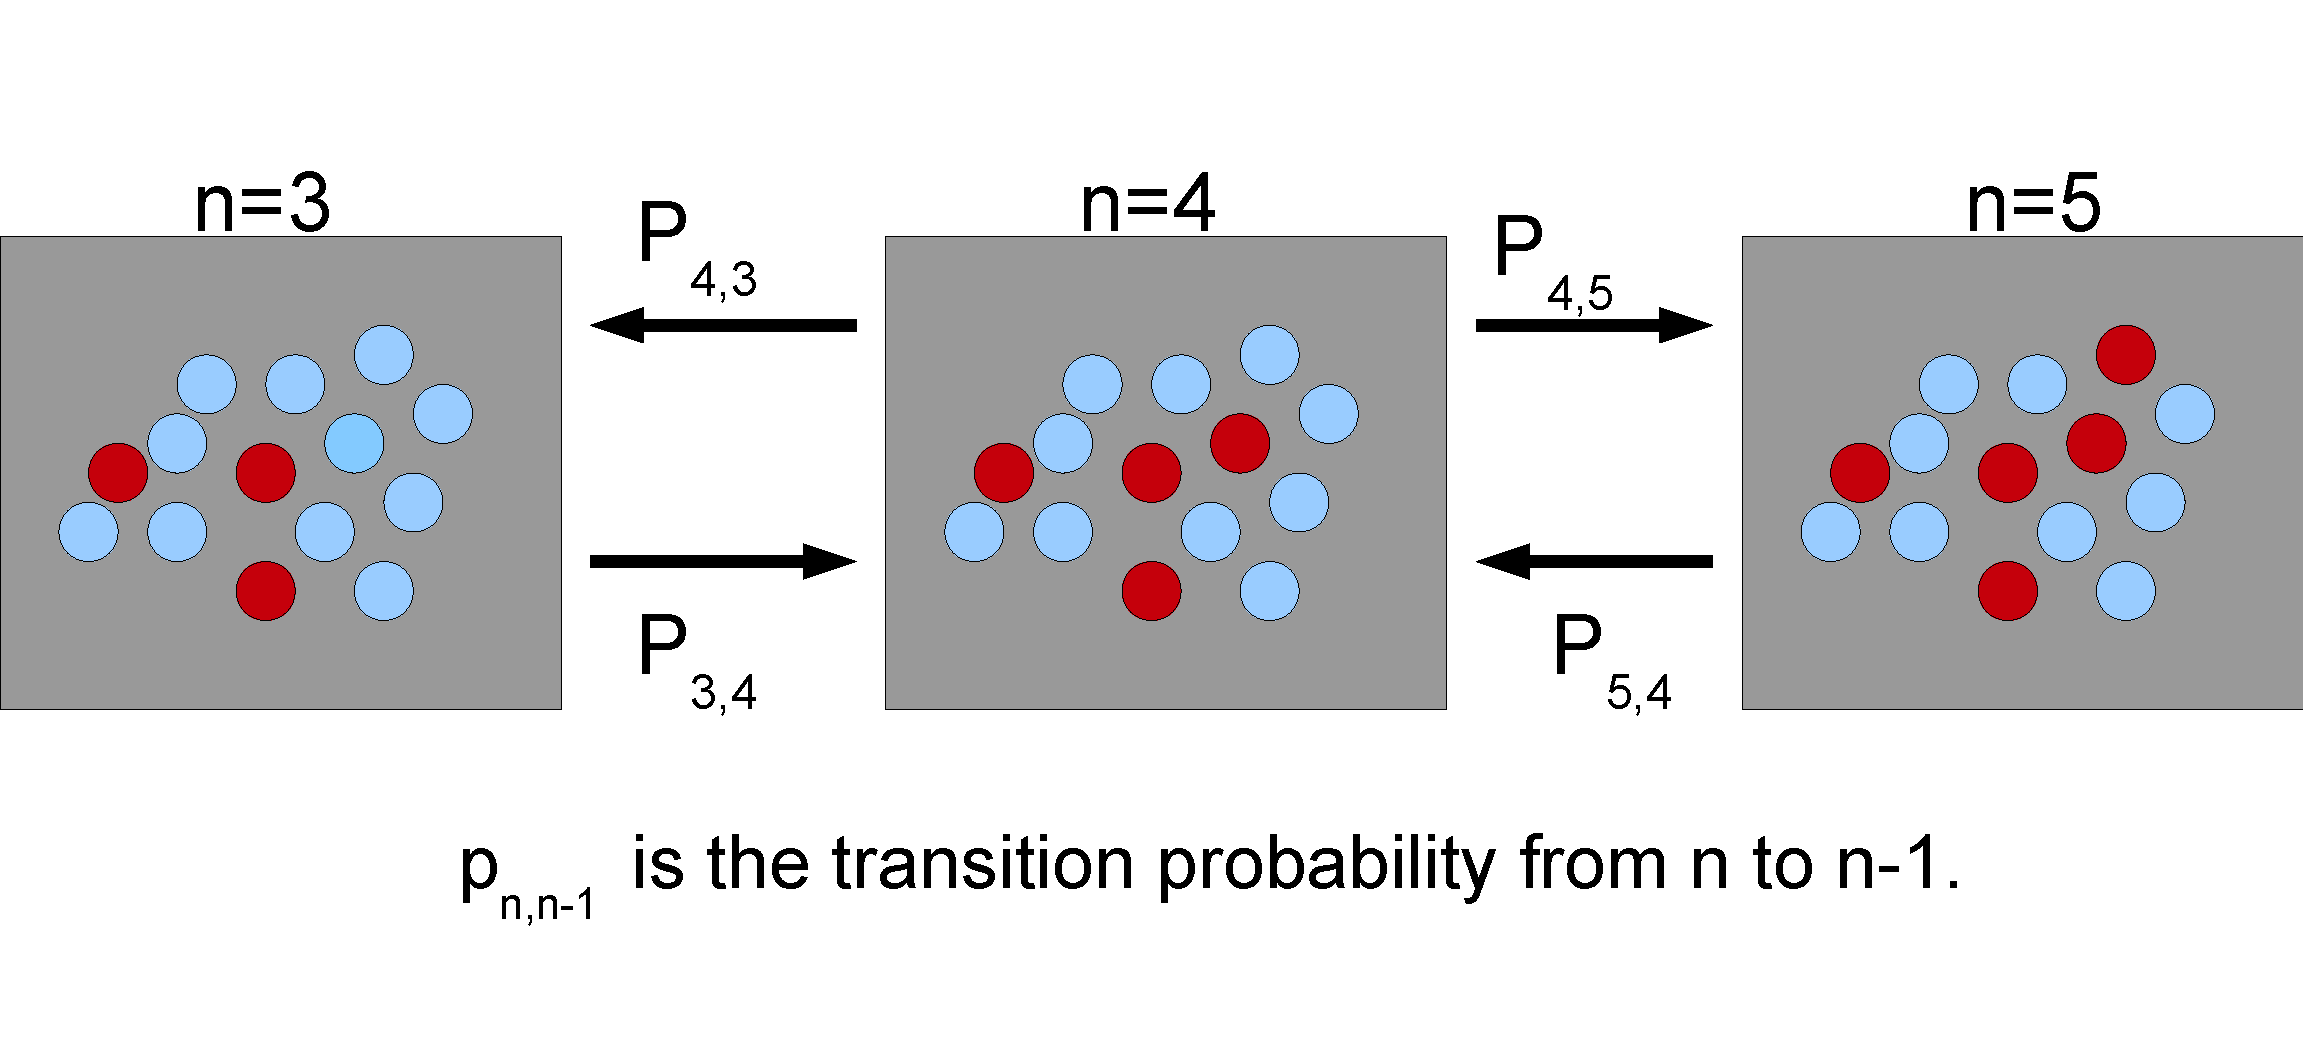
\includegraphics[width=9cm, height=7cm]{markovchainMoran.pdf}
    \fi
    \caption{Graph of transitions in a simple Moran process.}
    \label{Fig43}
  \end{center}
  \end{figure}

The probabilities of being selected for reproduction are $p_{A}$ and $p_{B}$, with the condition $p_{A}+p_{B}=1$, and each one is proportional to the type`s fitness, usually a linear function\cite{Shoresh2011}.
\begin{equation}
p_{A}=\frac{f_{A}n}{f_{A}n+f_{B}(N-n)} \;\; , \;\; p_{B}=\frac{f_{B}(N-n)}{f_{A}n+f_{B}(N-n)}.
\end{equation}  
The individual selected to die is chosen randomly, so the probabilities of  death for $A$ and $B$ are
\begin{equation}
\frac{n}{N}\;\;\; , \;\;\; \frac{N-n}{N}
\end{equation}
respectively. Therefore the probabilities of transition are
\begin{equation}
p_{n,n+1}=\frac{f_{A}n}{f_{A}n+f_{B}(N-n)} \frac{N-n}{N} \;\;\; , \;\;\; p_{n,n-1}=\frac{f_{B}(N-n)}{f_{A}n+f_{B}(N-n)}\frac{n}{N}
\end{equation}
and 
\begin{equation}
p_{n,n}=1-p_{n,n-1}-p_{n,n+1}
\end{equation}
In the next simulation Figure (\ref{Fig44}) we show the population of $A$ individuals as a function of time for a stochastic simulation of the Moran process. This stochastic simulation is a Monte Carlo step algorithm written in C++.
\begin{figure}[H]
 \begin{center}
    \leavevmode
    \ifpdf
      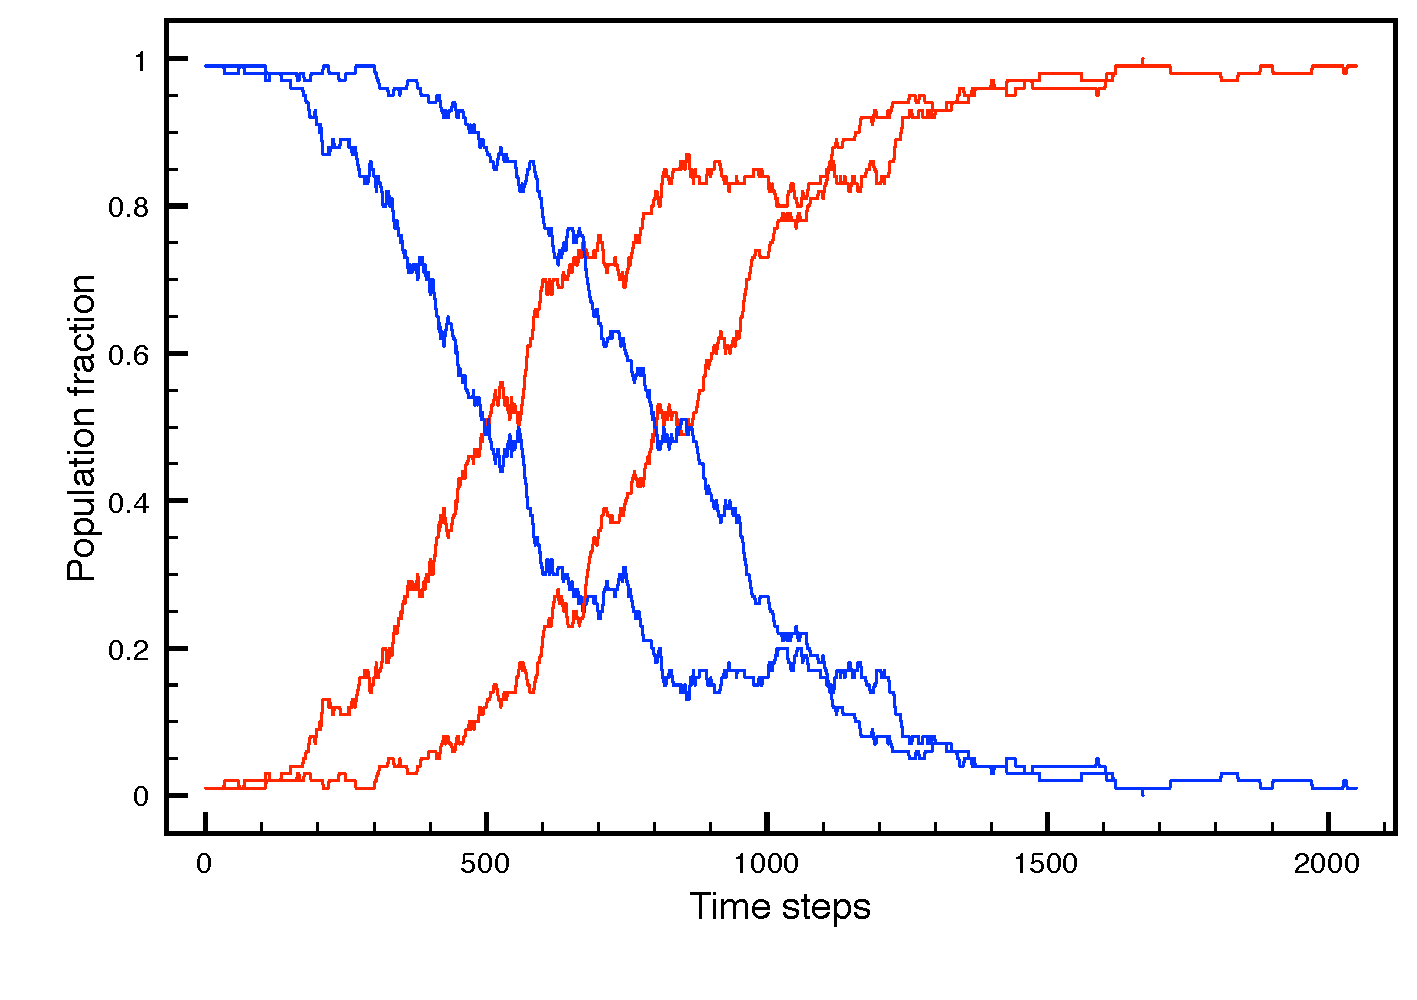
\includegraphics[width=10cm,height=7cm]{moransimulation.pdf}
    \else
     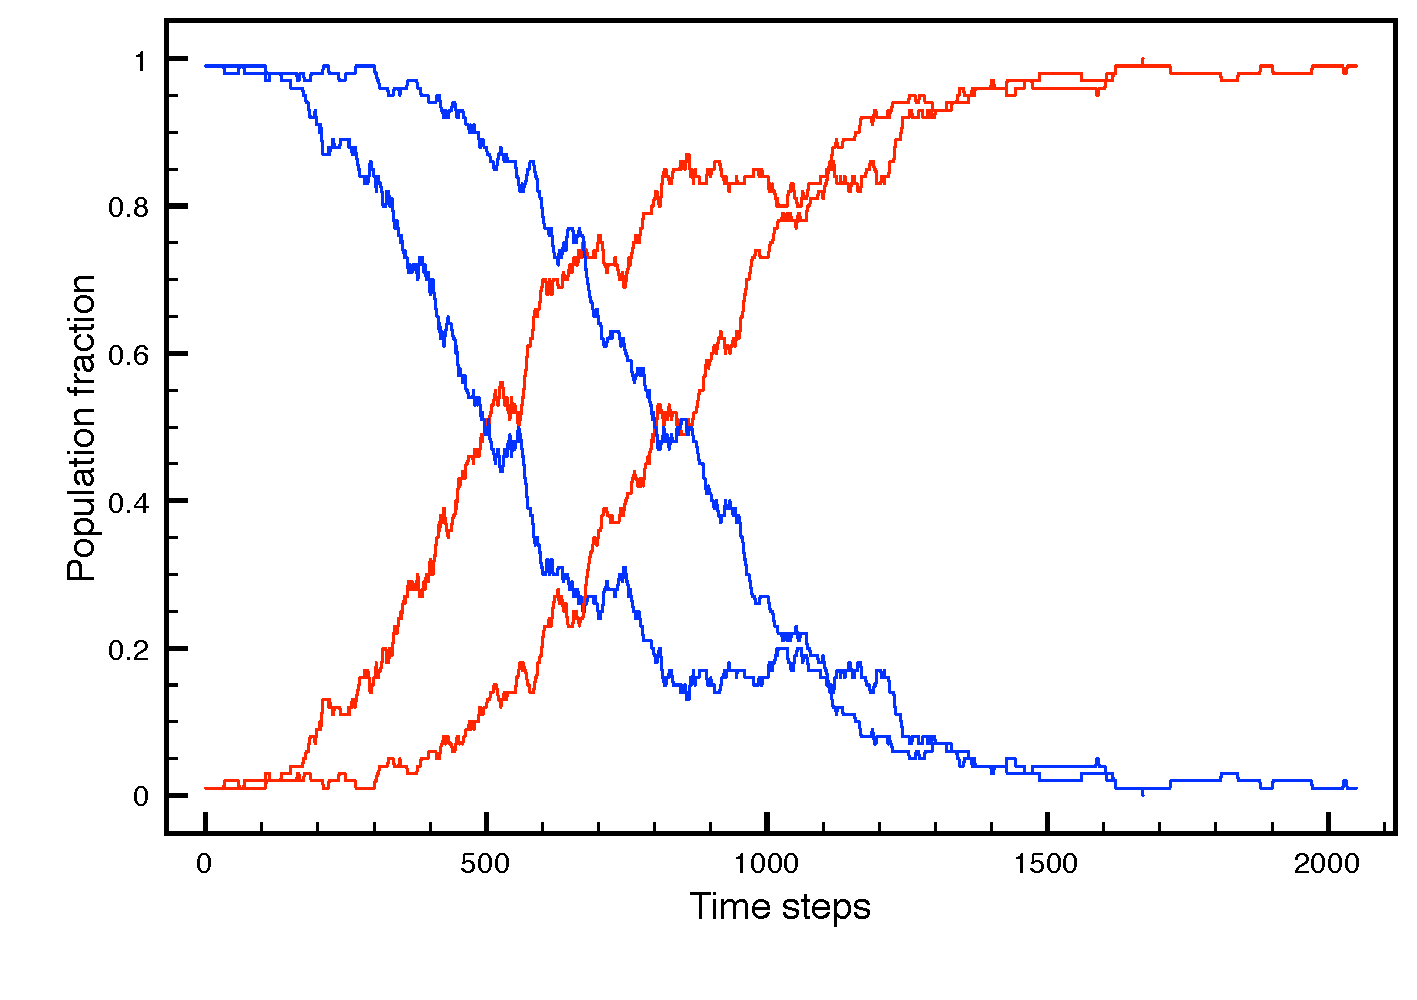
\includegraphics[width=10cm, height=7cm]{moransimulation.pdf}
    \fi
    \caption{\footnotesize Stochastic simulation of the Moran process for two executions of the program(Randomdrift.cpp). Blue line represents the population of $B$ individuals and red $A$ individuals. The fitnesses are $f_{A}=2$, $f_{B}=1$ and $N=100$ with an initial population of $A$ individuals $i=1$.}
    \label{Fig44}
  \end{center}
  \end{figure}
Now imagine that you have an experiment where you have $m>>1$ boxes with medium for growth bacterias, and in each of them you set the same initial conditions of population for two different types of bacterias. Then you let them compete until they have reached dominance in each box. 

\begin{figure}[H]
 \begin{center}
    \leavevmode
    \ifpdf
      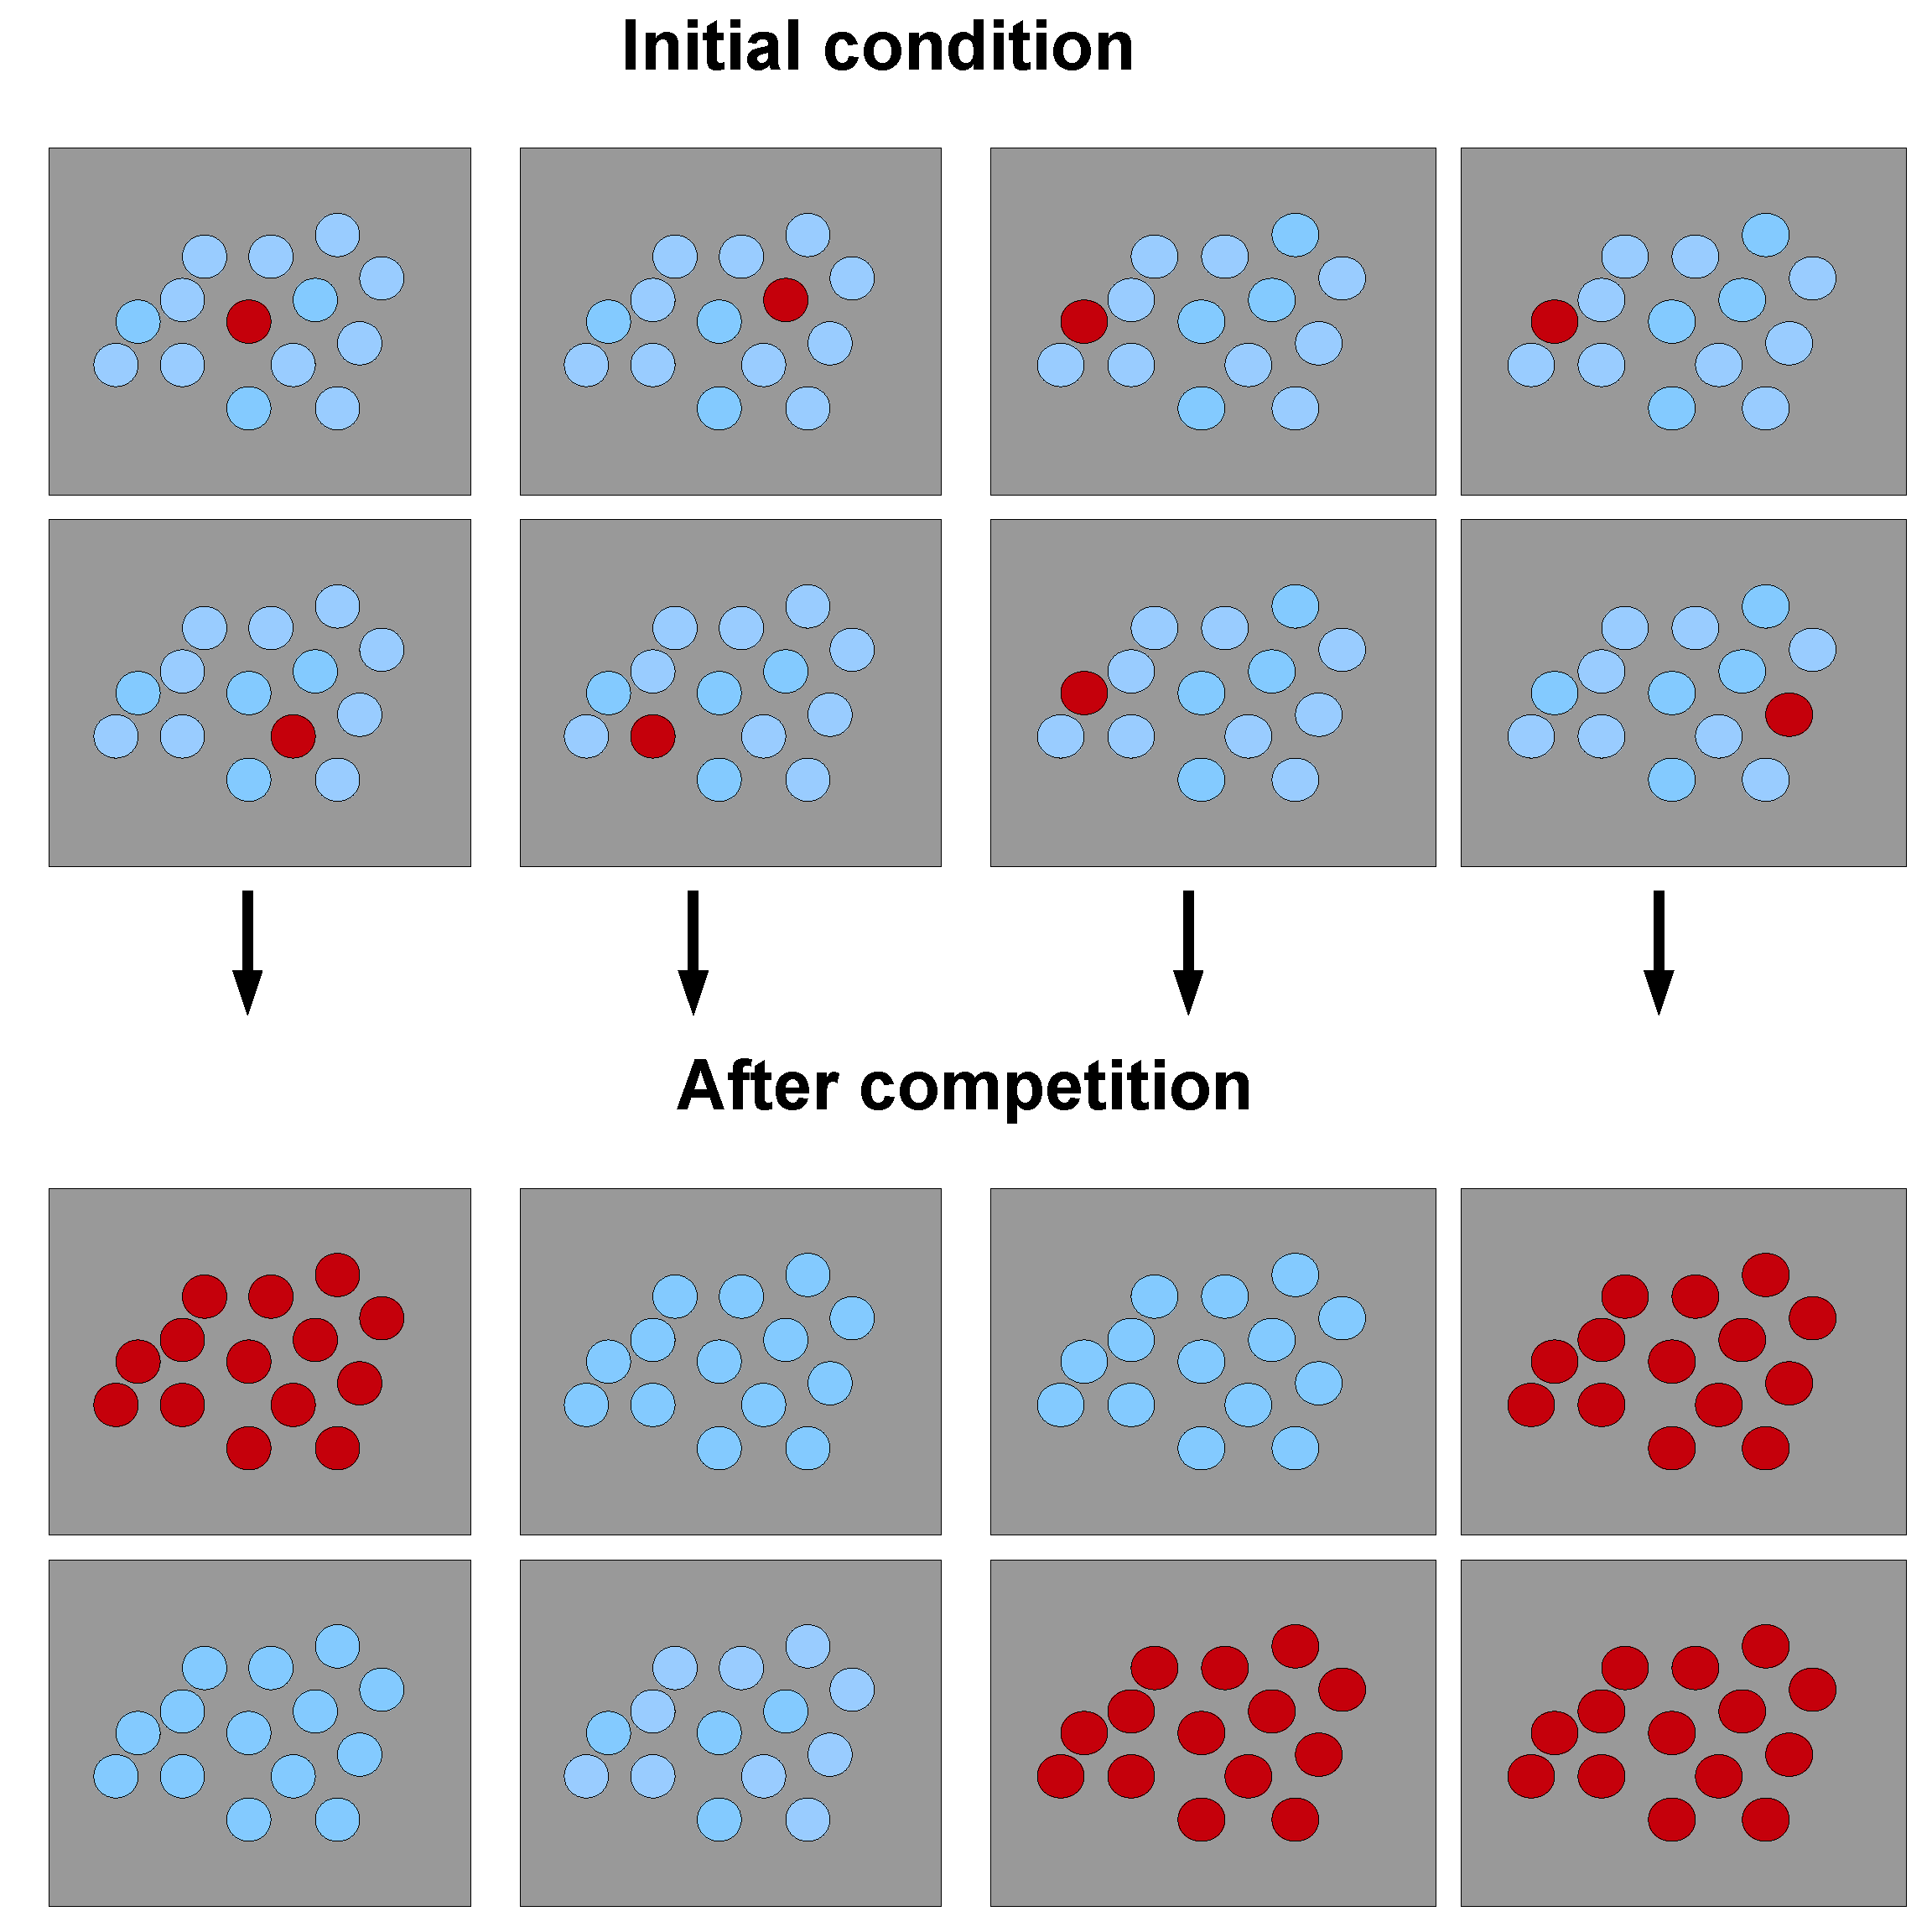
\includegraphics[width=10cm,height=7cm]{array.pdf}
    \else
     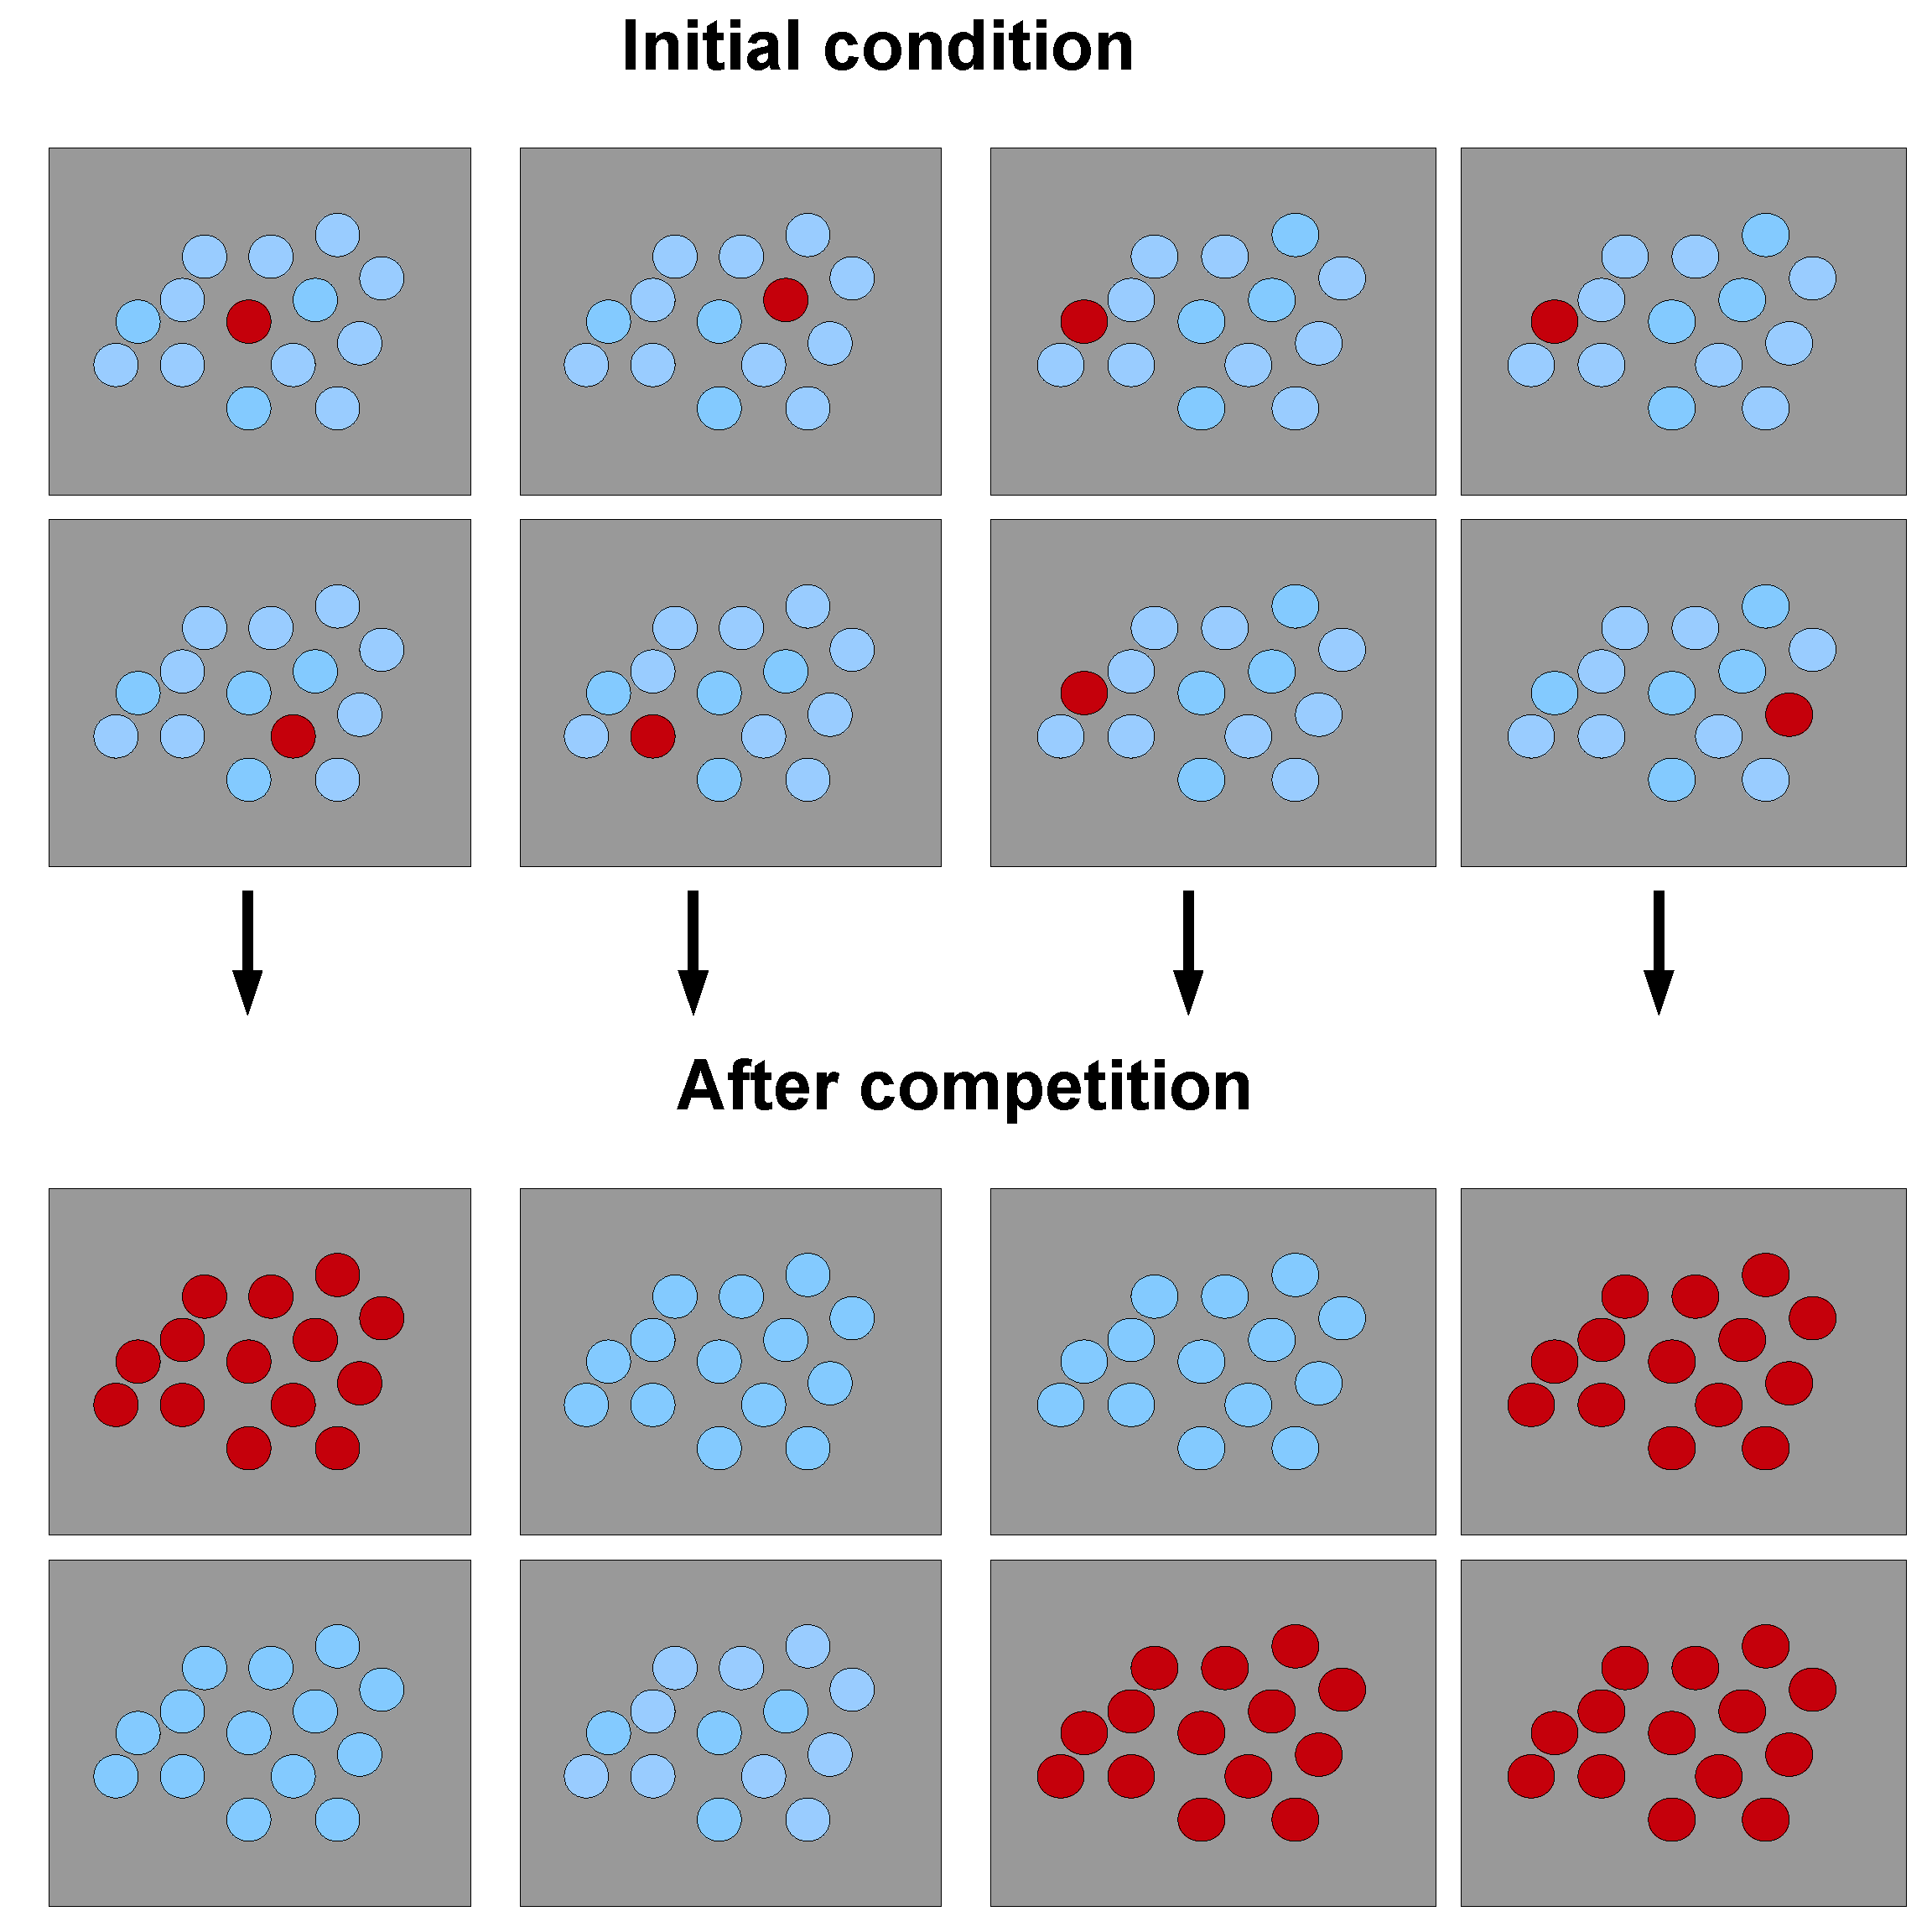
\includegraphics[width=10cm, height=7cm]{array.pdf}
    \fi
    \caption{\footnotesize Representation of several boxes with the same initial conditions that have different final states because of the stochasticity. The fraction of boxes where $A$ wins is called fixation probability.}  
    \label{Fig45}
  \end{center}
  \end{figure}


This is equivalent to running several times a simulation with the same initial conditions. Because of the stochasticity there is a fraction of boxes where each type dominate, but not in all, and this fraction is called the fixation probability for that respective type. It can be calculated analytically by solving the follow recurrence   equation for $\rho_{i}$ the fixation probability.
\begin{equation}
\rho_{i}=p_{i,i+1}\rho_{i+1}+p_{i,i-1}\rho_{i-1}+p_{i,i}\rho_{i}.
\end{equation} 
where $i$ is the initial population of individuals of type $A$.
\section{Neutral Drift}
In neutral drift two different types of organisms have equal fitnesses, so the dominance of one of them will depend only on the frequency of each type.  

The analytical procedure to find the probability of dominance is as follows: With a population of size $n$ and $i$ individuals of type $1$, the probabilities of choosing are: $i/n$ for type $1$ and $(n-i)/n$ for type $0$. Then the probability  that the population changes from $i$  to $i+1$ is 
\begin{equation}
p_{i,i+1}=\frac{i(n-i)}{n^2},
\end{equation}   
and from $i$ to $i+1$ is
\begin{equation}
p_{i,i-1}=\frac{(n-i)i}{n^2}.
\end{equation}
 The probability $\rho_i$ of fixation or dominance for the initial condition of $i$ individuals of type $1$ is $\rho_i=0$ if $i=0$ and $\rho_i=1$ if $i=n$; this is because  when an individual is chosen to die it is replaced by one of its same type. The probability $\rho_i$ is the sum of the probabilities of dominate from three events, that is
 \begin{equation}\label{4.9}
 \rho_i=p_{i,i}\rho_i + p_{i,i-1}\rho_{i-1} + p_{i,i+1}\rho_{i+1} \;\;\;\; i=1, 2, 3, ..., n-1
 \end{equation}  
 defining the new variables
 \begin{equation}
 y_i= \rho_{i}-\rho_{i-1}
  \end{equation}
  The series for $y_i$ is a geometric series
\begin{equation}
\sum_{i=1}^{n}y_i=\rho_{n}-\rho_{0}=1.
\end{equation} 
Since $p_{i,i-1}=p_{i,i+1}$ and $p_{i,i}=1-2p_{i,i+1}$, let us write equation \eqref{4.9} as
\begin{equation}
\rho_{i}2p_{i,i+1}=p_{i,i+1}(\rho_{i-1}+\rho_{i+1})
\end{equation}
\begin{equation}
\rho_{i}-\rho_{i-1}=\rho_{i+1}-\rho_{i}
\end{equation}
because $\rho_0 = 0$, then $y_i=\rho_1$ and $\sum_{i=1}^{n}y_i=\rho_{n}-\rho_{0}=n\rho_{1}$. To determine $\rho_i$ note that $\rho_i = \sum_{j=1}^{i}y_j =i\rho_1$, so finally
\begin{equation}
\rho_{i}=\frac{i}{n}.
\end{equation} 
This probability for neutral drift depends only on the initial population.
In the next Figure (\ref{Fig46}) it can be seen  that two simulations results in different population dominance.
\begin{figure}[H]
\begin{center}$
\begin{array}{cc}
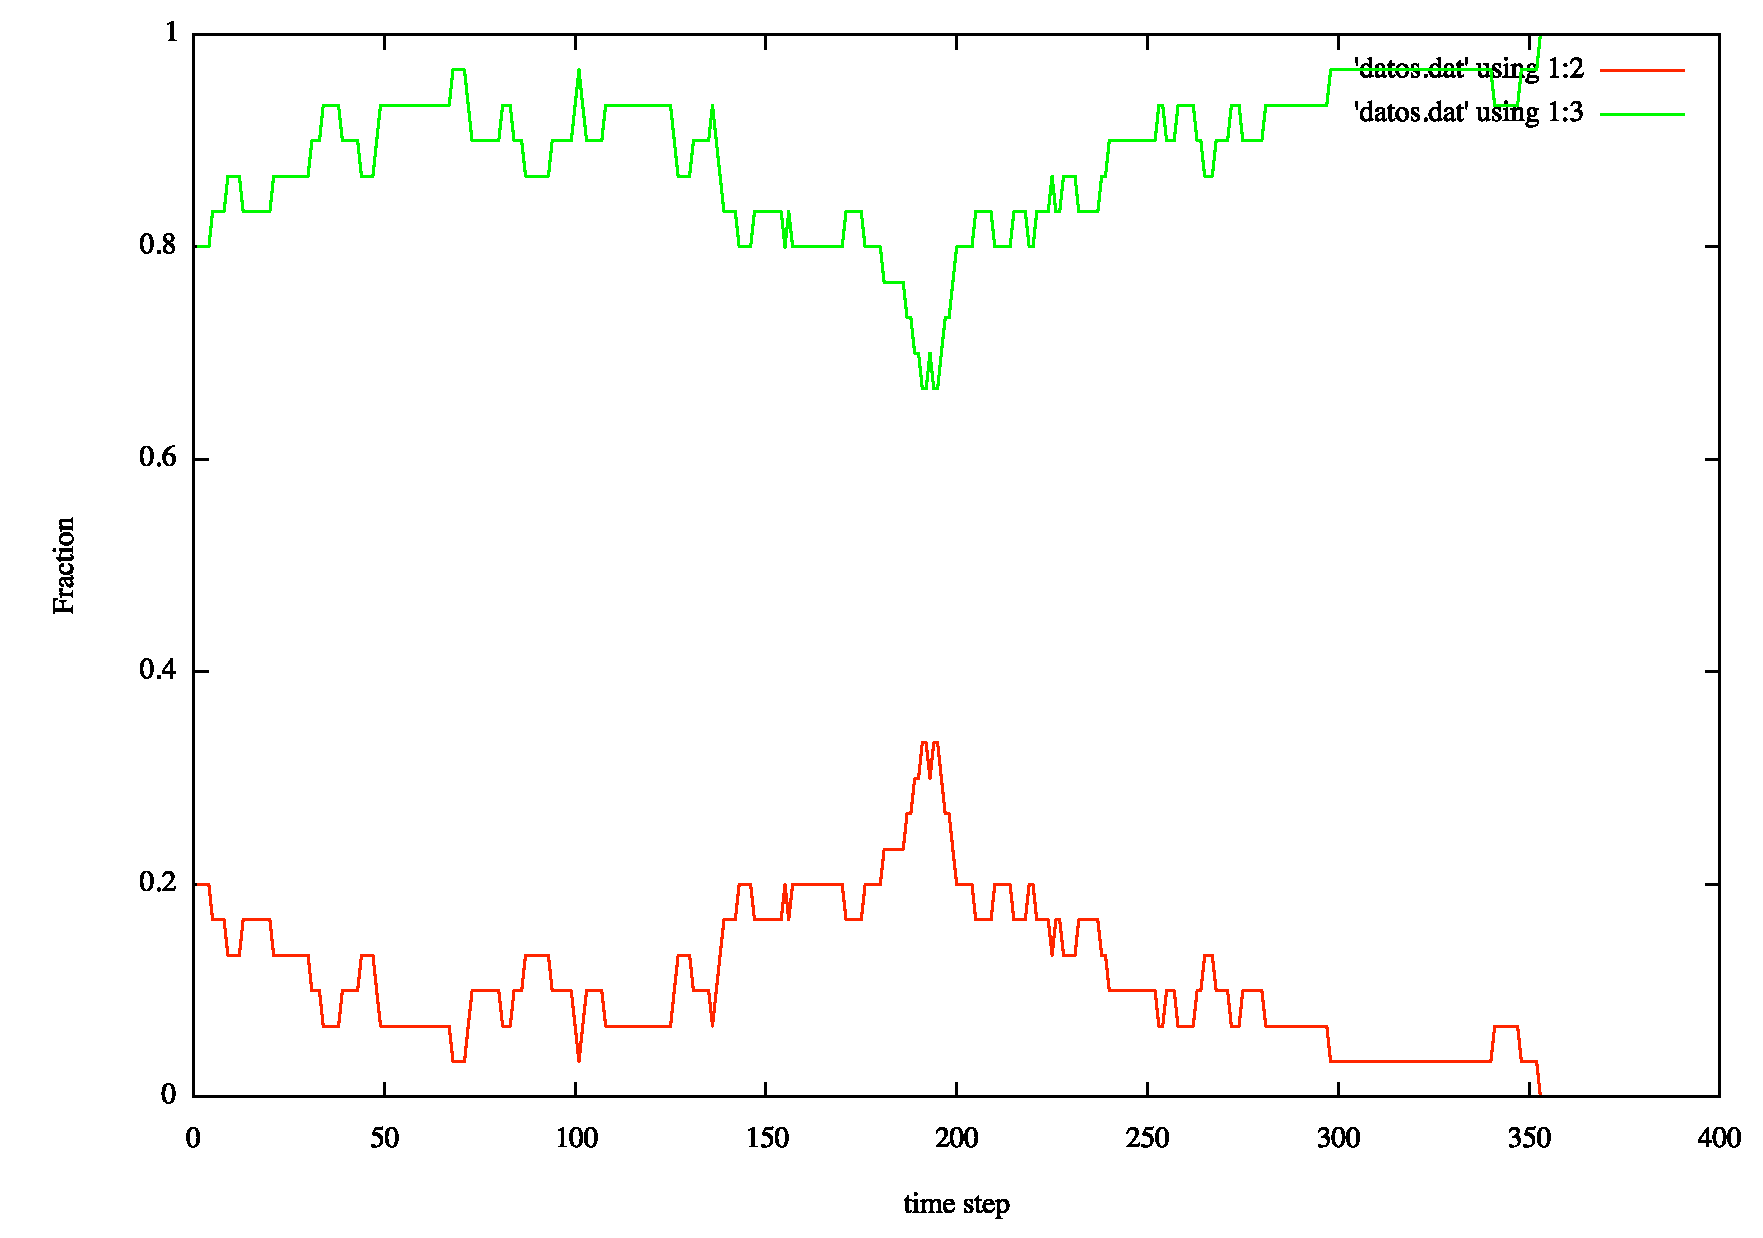
\includegraphics[width=2.5in]{bmoran1.pdf} &
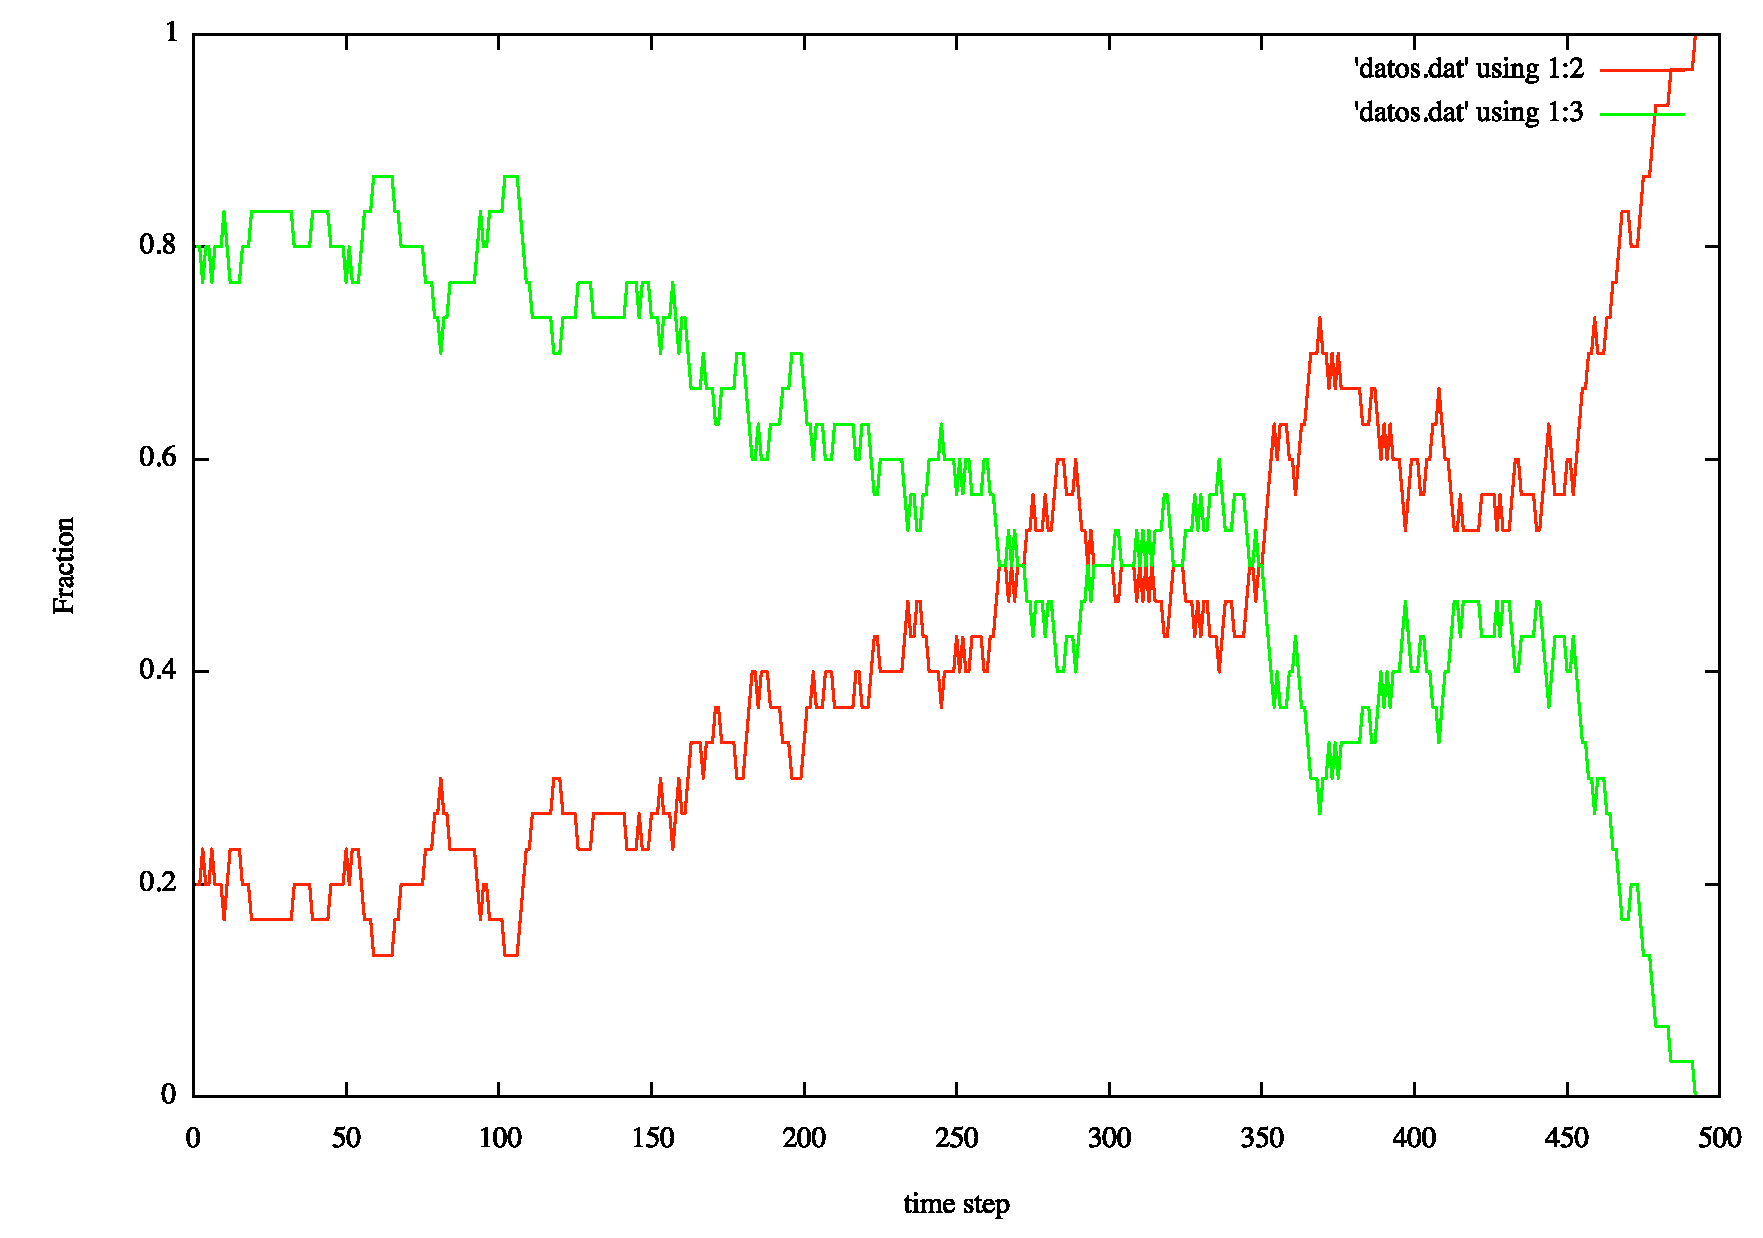
\includegraphics[width=2.5in]{bmoran.pdf}
\end{array}$
\end{center}
\caption{Two executions of the same neutral drift simulation with two different dominance result, which is due to stochasticity.}
\label{Fig46}
\end{figure}

This result for the probability $\rho_i$ can be corroborate  with the simulation shown in the next Figure (\ref{Fig47}).
\begin{figure}[H]
  \begin{center}
    \leavevmode
    \ifpdf
      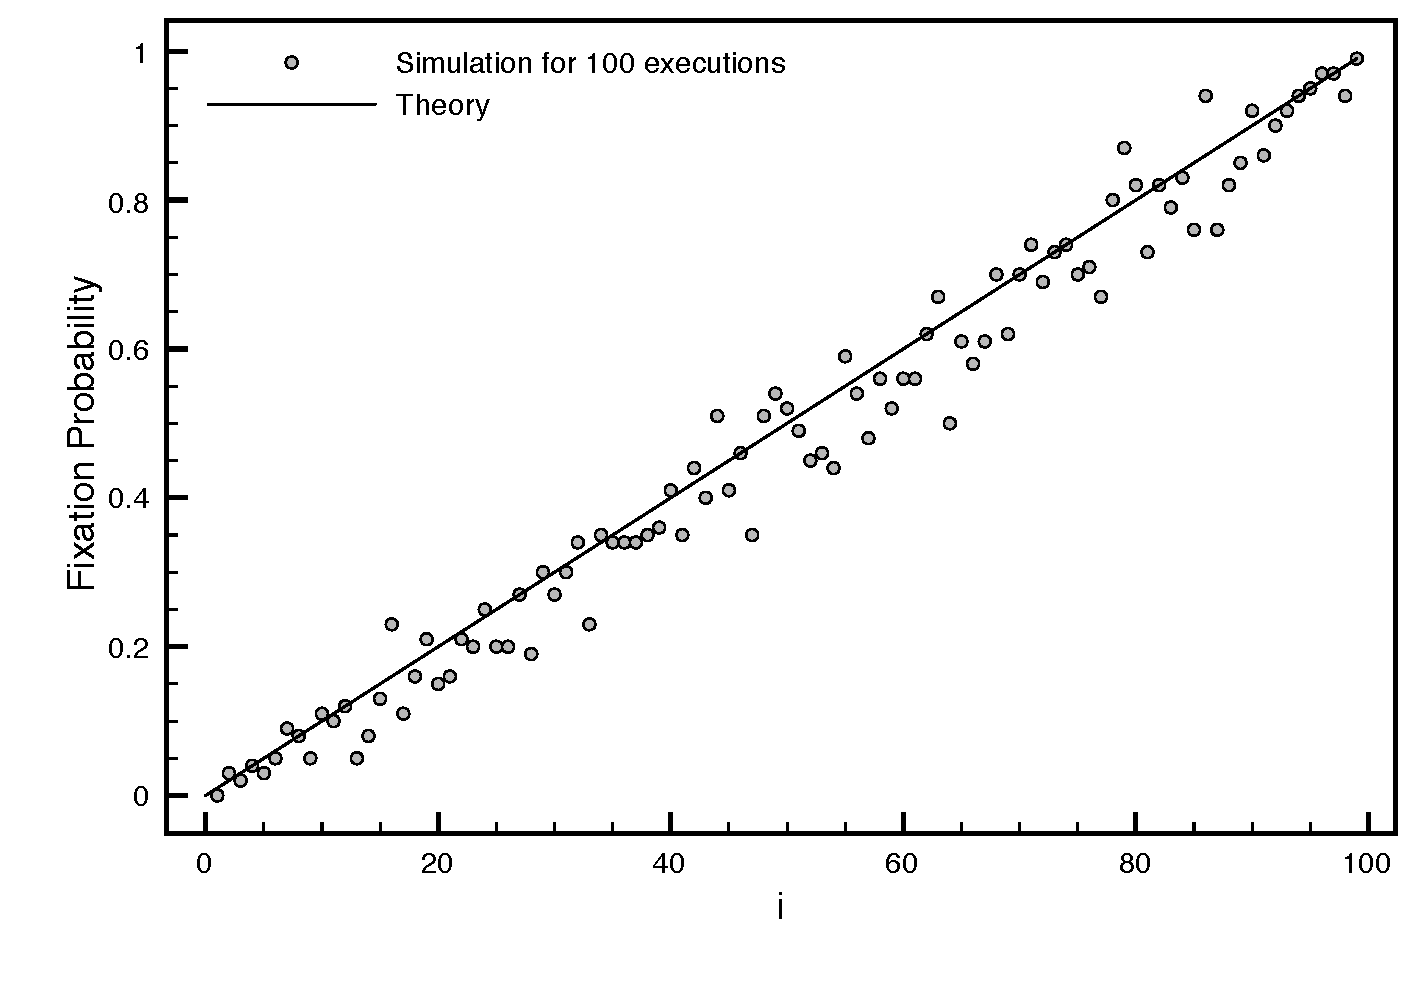
\includegraphics[width=8cm,height=7cm]{NeutralDriftPro.pdf}
    \else
      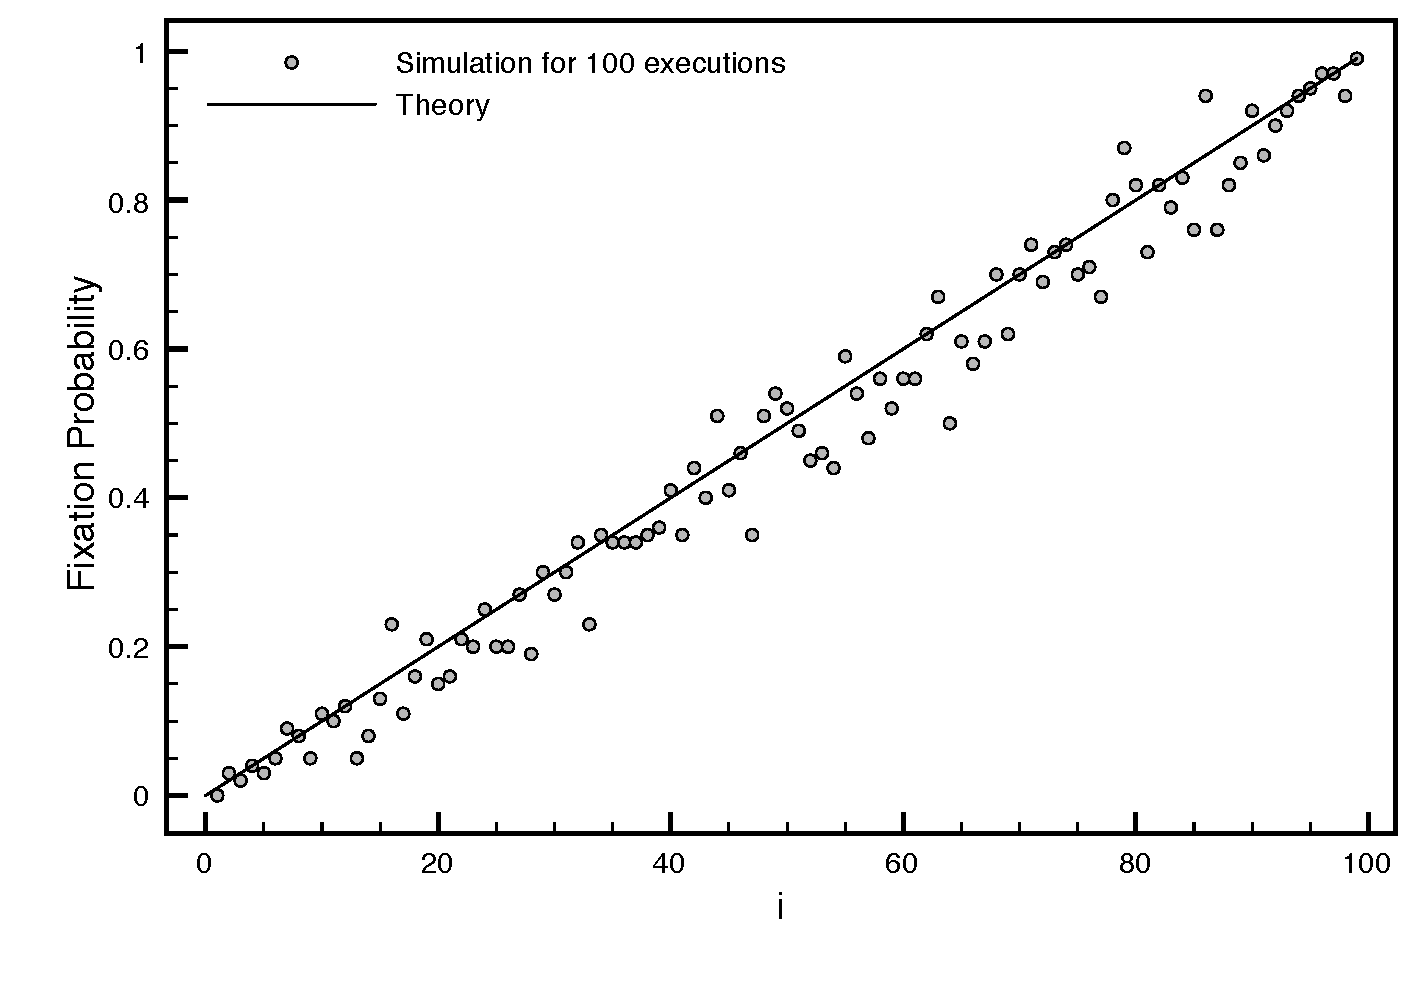
\includegraphics[width=8cm, height=7cm]{NeutralDriftPro.pdf}
    \fi
    \caption{Fixation probability in neutral drift as a function of initial population $i$ and size $n=100$.}
    \label{Fig47}
  \end{center}
  \end{figure}

\section{Random Drift}
We can perform the same calculation for the same process as before, but assuming that type $1$ has fitness $r$ and type $0$ fitness $1$. Then the probability that $1$ is chosen for reproduction is
\begin{equation}
\frac{ri}{ir+n-i}
\end{equation}
that $1$ is chosen for elimination is
\begin{equation}
\frac{i}{n}.
\end{equation}
Type $0$ has probability for reproduction $n-i/(ri+n-i)$ and $n-i/n$ for elimination. Therefore the probabilities of transition are
\begin{equation}
p_{i,i+1}=\frac{ri}{ri+n-i}\frac{n-i}{n}
\end{equation}
\begin{equation}
p_{i,i-1}=\frac{n-i}{ri+n-i}\frac{i}{n}
\end{equation}
\begin{equation}
p_{i,i}=1-p_{i,i+1}-p_{i,i-1}.
\end{equation}
Once again the conditions for fixation probabilities $\rho_{i}$ are $\rho_{0}=0$, $\rho_{n}=1$ and
\begin{equation}
\rho_{i}=p_{i,i}\rho_{i}+p_{i,i+1}\rho_{i+1}+p_{i,i-1}\rho_{i-1}.
\end{equation}
 With the new variable $y_{i}=\rho_{i}-\rho_{i-1}$ we can write equation (18) as
 \begin{equation}
 y_i = y_{i+1}\frac{p_{i,i+1}}{p_{i,i-1}}=y_{i+1}\frac{ri}{n-i}\frac{n-i}{i}
 \end{equation}
 then $y_{i+1}=\frac{1}{r}y_i$, and these lead to
\begin{equation}
y_i =\frac{1}{r^{i-1}}\rho_1
\end{equation}  
since $1=\rho_1 (1+\sum_{m=1}^{n-1}\frac{1}{r^{m}} )$ and $\rho_i=\rho_1 (1+\sum_{j=1}^{i-1}\frac{1}{r^{j}} )$, the fixation probability is
\begin{equation}
\rho_{i}=\frac{1+\sum_{j=1}^{i-1}\frac{1}{r^j}}{1+\sum_{m=1}^{n-1}\frac{1}{r^m}}.
\end{equation}
In this expression we have a telescopic series. The sum value for a telescopic series is
\begin{equation}
\sum_{i=0}^{n}\frac{1}{x^n}=\frac{1-\frac{1}{x^{n+1}}}{1-\frac{1}{x}}.
\end{equation}  
Therefore the probability of fixation for type $1$ starting in state $i$ is
\begin{equation}\label{4.25}
\rho_i = \frac{1-1/r^i}{1-1/r^n}.
\end{equation}
This result can be checked in a Moran process simulation where  the fixation probability is measured as a function of $r$. In the Figure (\ref{Fig48}) below  the analytical curve and the stochastic measures are shown.
\begin{figure}[H]
  \begin{center}
    \leavevmode
    \ifpdf
      \includegraphics[width=8cm,height=7cm]{Plot.pdf}
    \else
      \includegraphics[width=8cm, height=7cm]{Plot.pdf}
    \fi
    \caption{Fixation probability in random drift as a function of $r$ in a population of size $n=100$ and initial state $i=50$ ,where each point was calculated with $1000$ executions. The line represents the analytical model.}
    \label{Fig48}
  \end{center}
  \end{figure}
In the case where type $0$ has a fitness $s$, the fixation probability Eq. \eqref{4.25} is written as
\begin{equation}
\rho_i = \frac{1-(s/r)^i}{1-(s/r)^n}
\end{equation}
\section{Fixation Times}
Fixation time is the average time that the competition system takes to get to one of the two absorbing states\cite{Antal, Traulsen2009}. Because of the stochasticity of the system the time for reaching these states is a distribution, where each time $t$ for reaching an absorbing state($0$ or $n$) starting from $i$ type $A$ individuals has a probability $P_i ^{n,0} (t)$. As for fixation probabilities, for $P_i ^{n,0} (t)$ there is also a recurrence equation, that is the probability sum of three different events:
\begin{itemize}
\item The probability of jump to state $i-1$ in the first time step, and from there it takes a time $t-1$ with probability $P_{i-1}^{n,0}(t-1)$ for reaching the absorbing state.
\item The probability of jump to state $i+1$ in the first time step, and from there it takes a time $t-1$ with probability $P_{i+1}^{n,0}(t-1)$ for reaching the absorbing state.
\item The probability of staying in state $i$ in the first time step, and from there it takes a time $t-1$ with probability $P_{i}^{n,0}(t-1)$ for reaching the absorbing state.
\end{itemize}
 The recurrence equation is
 \begin{equation}
 P_i ^{n,0} (t)= P_{i,i-1}P_{i-1}^{n,0}(t-1)+P_{i,i+1}P_{i+1}^{n,0}(t-1)+P_{i,i}P_{i}^{n,0}(t-1).
 \end{equation}  
The probability of time $t$ for reaching state $n$ is $P_{i}^{n}(t)$, and the recurrence equation for the dominance of type $A$ is\cite{Antal}
 \begin{equation}\label{4.27}
 P_i ^{n} (t)= P_{i,i-1}P_{i-1}^{n}(t-1)+P_{i,i+1}P_{i+1}^{n}(t-1)+P_{i,i}P_{i}^{n}(t-1)
 \end{equation} 
 with the boundary conditions  $P_{0}^{n}(t)=0$ and $P_{n}^{n}(0)=1$. The average absorbsion time is
 \begin{equation}
 t_i = \frac{\sum\limits_{t=0}^{\infty}tP_{i}^{n}(t)}{\sum\limits_{t=0}^{\infty}P_{i}^{n}(t)},
 \end{equation}
 where $\sum\limits_{t=0}^{\infty}P_{i}^{n}(t)=\rho_i $.
 Multiplying Eq. \eqref{4.27} by $t$,  sum it and applying the  identity
 \begin{equation}
 \sum\limits_{t=0}^{\infty}tP_{i}^{n}(t-1)=\rho_{i}(t_i + 1).
 \end{equation}
 We get
 \begin{equation}
 t_i \rho_i =P_{i,i-1}\rho_{i-1}(t_{i-1}+1) + P_{i,i+1}\rho_{i+1}(t_{i+1}+1) + P_{i,i}\rho_{i}(t_{i}+1).
 \end{equation}
 Replacing $\tau_{i}=t_i \rho_i$ and using the recurrence equation Eq. \eqref{4.9}, the above equation becomes
 \begin{equation}
 -\rho_i =P_{i,i-1}\tau_{i-1}-\tau_1(P_{i,i+1}+P_{i,i-1})+P_{i,i}\tau_{i+1}.
 \end{equation}
 Because this is a recurrence relation we can use $s_{i}=\tau_i -\tau_{i+1}$, and get
 \begin{equation}
 s_{i}=\frac{P_{i,i-1}}{P_{i,i+1}}s_{i-1}+\frac{\rho_i}{P_{i,i+1}}.
 \end{equation}
 since $s_{0}=-\tau_1$, and iterating some times:
 \begin{equation*}
 \begin{split}
s_1 = & \frac{\rho_1}{P_{1,2}} - t_1 \rho_1\frac{P_{1,0}}{P_{1,2}} \\
:\\
s_3 =& \frac{P_{3,2}}{P_{3,4}}\left[\frac{P_{2,1}}{P_{2,3}}\left( \frac{\rho_{1}}{P_{1,2}}+  s_0 \frac{P_{1,0}}{P_{1,2}}\right)+ \frac{\rho_2}{P_{2,3}}\right] + \frac{\rho_{3}}{P_{3,4}}.
 \end{split}
\end{equation*}
Then by induction:
\begin{equation}\label{4.33}
s_{i}=s_0 \prod\limits_{j=1}^{i}\frac{P_{j,j-1}}{P_{j,j+1}} + \sum\limits_{j=1}^{i}\frac{\rho_j}{P_{j,j+1}}\prod\limits_{m=j+1}^{i}\frac{P_{m,m-1}}{P_{m,m+1}},
\end{equation}
with the convention that $\prod\limits_{i+1}^{i}\frac{P_{m,m-1}}{P_{m,m+1}} =1$.
Now to determinate $t_1$, we use the fact that $\sum\limits_{n=1}^{i}s_n = \tau_1-\tau_{i+1}$, and $\tau_n=0$.Then 
\begin{equation}
\tau_1=\sum\limits_{i=1}^{n-1}s_i,
\end{equation}
and using Eq. \eqref{4.33}
\begin{equation}
\tau_1\left(1+ \sum\limits_{i=1}^{n-1}\prod\limits_{j=1}^{i}\frac{P_{j,j-1}}{P_{j,j+1}}\right)=\sum\limits_{i=1}^{n-1}\sum\limits_{j=1}^{i}\frac{\rho_j}{P_{j,j+1}}\prod\limits_{m=j+1}^{i}\frac{P_{m,m-1}}{P_{m,m+1}},
\end{equation}
Finally $t_{1}$ is
\begin{equation}\label{4.36}
t_1=\sum\limits_{i=1}^{n-1}\sum\limits_{j=1}^{i}\frac{\rho_j}{P_{j,j+1}}\prod\limits_{m=j+1}^{i}\frac{P_{m,m-1}}{P_{m,m+1}}.
\end{equation}
With this result we can determinate the expression for the fixation time $t_{i}$ of $i$ initial $A$ individuals. We can see that 
\begin{equation}
\sum\limits_{k=1}^{i-1}s_k=\tau_1 -\tau_i,
\end{equation}   
but in this equation we can replace
\begin{equation*}
\sum\limits_{k=1}^{i-1}s_k=\sum\limits_{k=1}^{n-1}s_k -\sum\limits_{k=i}^{n-1}s_k
\end{equation*} 
to get the relation
\begin{equation}
\tau_i=\sum\limits_{k=i}^{n-1}s_k
\end{equation}
where replacing $s_k$.  $t_i$ is
\begin{equation}\label{4.39}
t_i=-\frac{\rho_1 t_1}{\rho_i}\sum\limits_{k=i}^{n-1}\prod\limits_{j=1}^{k}\frac{P_{j,j-1}}{P_{j,j+1}} + \sum\limits_{k=i}^{n-1}\sum\limits_{j=1}^{k}\frac{\rho_j}{\rho_i P_{j,j+1}}\prod\limits_{m=j+1}^{k}\frac{P_{m,m-1}}{P_{m,m+1}}.
\end{equation}
For random drift $t_1$ and $t_i$ simplify to:
\begin{equation}
t_{1}=\frac{n}{1-(\frac{s}{r})^n}\sum\limits_{k=1}^{n-1}(\frac{s}{r})^k \sum\limits_{l=1}^{k}\left(1-(\frac{s}{r})^l \right)\left(\frac{1}{n-1}+\frac{s}{rl}\right),
\end{equation}
\begin{equation}
t_i=t_1 -t_1\left(\frac{1-(s/r)^n}{1-(s/r)^i}\right)+\frac{n}{r(1-(s/r)^i)}\sum\limits_{k=i}^{n-1}\sum\limits_{l=1}^{k}\left(1-(s/r)^l\right)\frac{(rl+s(n-l))}{l(n-l)}
\end{equation}
If we observe carefully these expressions, it can be seen that $t_1$ is shorter as fitness $r$ increases. In the case for $t_{i}$, the larger the initial population $i$, the shorter the average time for reaching dominance. These interpretations are consistent  with those from Eq. \eqref{3.12}. 
% ------------------------------------------------------------------------


%%% Local Variables: 
%%% mode: latex
%%% TeX-master: "../thesis"
%%% End: 

%%% Thesis Introduction --------------------------------------------------
\chapter{Game Theory, Cooperation and Fitness}
\ifpdf
    \graphicspath{{GameTheory/Figs/PNG/}{GameTheory/Figs/PDF/}{GameTheory/Figs/}}
\else
    \graphicspath{{GameTheory/Figs/EPS/}{GameTheory/Figs/}}
\fi
 Evolution is usually described as a fierce competition between individuals, that leads to a selfish behavior as, for example  the competition among lions for females, but it has been seen that in many biological systems evolution leads also to cooperative behaviors between individuals\cite{Dunny2008}, for example when bacteria gather in a biofilm to help each other, or in cooperation among humans in a work team. 

Natural selection can leads to cooperation if it  implies a higher benefit than that when individuals are selfish. A population of only cooperators can then be invaded by a cheater if behaving like that has more benefit, or the opposite situation where cheaters are invaded by cooperators. The mechanisms that leads to one of those behaviors in a population of individuals depend on the biological system.   

Some scientist have proposed models to described the selection of cooperation and behavior interactions among organisms. This science field has been called evolutionary game theory. For example  Martin A. Nowak,  who has worked in evolutionary dynamics,  has proposed five mechanisms for the evolution of cooperation based on  game theory, where the benefit of cooperating or defecting is related to the fitness of individuals\cite{Nowak2011,Shoresh2011}. The mechanisms are: kin selection, direct reciprocity, indirect reciprocity, network reciprocity and group selection. The last one , group selection, describes the evolution of cooperation in individuals of different groups that are on competition.

%The group selection model is based in a fixed grade of cooperation, which means that it is deterministic, but in a biological system each individual is going to cooperate in different degrees due to the phenotype variability, although in isogenic groups. This is an effect of the gene expression noise. For example the noise expression noise affects the fitness of organisms when its fitness depends of some phenotype advantage that is generate by a gene or group of genes, the increase in the gene noise expression can leads to a decrement of the total fitness.  Including phenotypic variability to Nowak's model allows an approach more realistic to the evolution of cooperation, and detailed simulations of competition populations of cooperators and defectors would allow to characterize the importance of phenotypic variability and its utility as an evolutive strategy.  


Differences between evolutionary game theory and classical game theory are essential. Classical theory considers rational players thinking about others strategies, which becomes an infinite iterating game \cite{Traulsen2009}. In evolutionary game theory organisms are considered not rational, and strategies spreads depending on the utility that they give to the players; they can be imitated or inherited.   

%%% ----------------------------------------------------------------------
\section{Fitness Due to Cooperate-Defect}
When organisms have interaction in some environment where each of them have the possibility of different strategies or behaviors, from those interactions each individual in the biological system will get an utility. In the simplest situation imagine  two different organisms that have the option of two behaviors: cooperate and defect. For example in sea there are two fish, the white shark and Pilot fish, that cooperate each other.  The White shark can let Pilot fish to eat the parasites on its skin. Therefore it is said that if the shark lets it eat from its skin, it cooperates, and the Pilot fish cooperates when it cleans shark's skin. 
\begin{figure}[H]
 \begin{center}
    \leavevmode
    \ifpdf
      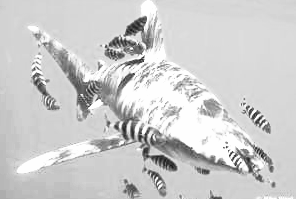
\includegraphics[width=10cm,height=7cm]{mutualism.png}
    \else
     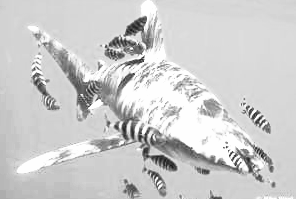
\includegraphics[width=10cm, height=7cm]{mutualism.png}
    \fi
    \caption{\footnotesize Illustration of cooperation between White shark and Pilot fish(www.pioneermindset.wordpress.com).}  
    \label{Fig51}
  \end{center}
  \end{figure}

The utilities of this interaction can be visualize in a payoff matrix.

\begin{equation*}
\begin{matrix}
    & Pilot\; fish \\
 White\; shark & {\bordermatrix{~ & C& D \cr
                            C & A_{shark} & B_{shark} \cr
                            D & C_{shark} & D_{shark} \cr}} 
 \end{matrix}\;\;\;
 \begin{matrix}
    & White \; shark \\
 Pilot\; fish & {\bordermatrix{~ & C& D \cr
                            C & A_{fish} & B_{fish} \cr
                            D & C_{fish} & D_{fish} \cr}} 
\end{matrix}
\end{equation*}

Where the elements of the left hand matrix are the utilities for the shark,  and the right hand matrix has the utilities for the Pilot fish. This utility of the interaction represents a contribution to the fitness of each individual. For the White shark, it will get a skin clean of parasites, increasing its life time and possibility of reproduction. For the Pilot fish, it will get a source of food and protection from bigger predators. Both organisms can get a larger per capita reproduction rate from the altruistic act.

As we see in the last matrices, a matrix  is needed  for the utilities of each individual, but in the case where the utilities from the interaction are symmetric just one payoff matrix  is used:
\begin{equation}\label{5.1}
\bordermatrix{~ & C & D \cr
             C & R & S \cr
              D & T & P \cr}. 
\end{equation}
An example of this symmetric situation, is  a group of bacteria that have pair interactions, where each time that two bacteria meet they have the options of cooperate producing an enzyme for processing food, or defect taking food without  spend energy producing the enzyme. This interaction has a benefit $b$ and a cost $c$ for producing the enzyme. Thus, the  payoff matrix of this game is
\begin{equation*}
\bordermatrix{~ & C & D \cr
             C & b-c & -c \cr
              D & b & 0\cr}, 
\end{equation*}
where it can be observed that the strategy with the largest utility is defecting, but if this strategy invades the group, no bacterium will have a benefit.

Now let us examine how the process of selection works in game theory. Imagine a group of size $n$ with $i$ individuals that cooperate and $n-i$ that defect. The expected payoff $\pi_{C}$ of cooperators due to pairwise encounters with the rest of individuals in the group is
\begin{equation}
 \pi_{C}=\frac{R(i-1)+S(n-i)}{n-1}.
\end{equation}
This average utility will represents a reproductive rate for the individuals with the strategy of cooperation. Usually fitness is  a linear function like
\begin{equation}
f_{C}=1-w+w\pi_{C},
\end{equation}
where $w$ is called the intensity of selection, and represents how much the game contributes to selection process. For example, for $w=0$ the competition reduces to neutral drift and the game has not effect on the fitness.



There is another function of fitness that is usually used, this is an exponential function of expected payoff $\pi_{C}$,
\begin{equation}
f_{C}=e^{w\pi_{C}}.
\end{equation}
This function is usually used for analytical results of fixation probabilities when intensity of selection is large.

Then in summary, in a group of size $n$ and $i$ cooperators, the expected payoff and fitness for a defector will be:
\begin{equation}
\pi_{D}=\frac{Ti + P(n-i-1)}{n-1}\;\:\:\; f_{D}=1-w+w\pi_{D}.
\end{equation} 
 
Systems where there is not fitness due to interaction and it is intrinsic to each type of organism, as random drift also can be written in a payoff matrix, and doing the algebraic calculations get same transitions probabilities. Then for neutral drift
\begin{equation*}
\bordermatrix{~ & A & B \cr
             A & 1 & 1 \cr
              B & 1 & 1 \cr} 
\end{equation*}
 and for random drift
 \begin{equation*}
\bordermatrix{~ & A & B \cr
             A & r & r \cr
              B & s & s \cr}. 
\end{equation*}
Let us calculate $\pi_A$ in the case that $w=1$ for random drift.
\begin{equation*}
f_{A}=\pi_A=\frac{r(i-1)+r(n-i)}{n-1}=r\;\; and \;\; f_{B}=s
\end{equation*}
We have seen above examples of cooperation among different species, but the interest of this work is to study how cooperation evolves among individuals of the same specie, as humans or yeast. 

 
\section{Fixation Probability}
For fixation probability the same procedure is used  as for random drift, with the difference that $f_{C,D}$ is a function of the frequency $i$. First of all, we should define $P_{i,i+1}$ and $P_{i,i-1}$:
\begin{equation}
P_{i,i+1}=\frac{f_{C}i}{f_{C}i+f_{D}(n-i)}\frac{n-i}{n}.
\end{equation} 


Again the equation for $\rho_{i}$ is 
\begin{equation}\label{5.9}
\rho_{i}=\rho_{i}P_{i,i} + \rho_{i-1}P_{i,i-1} + \rho_{i+1}P_{i,i+1}
\end{equation}   
replacing the new variable $x_{i}=\rho_{i}-\rho_{i-1}$.
\begin{equation}
P_{i,i-1}x_{i}=P_{i,i+1}x_{i+1}
\end{equation}
with the conditions
\begin{equation}
 x_0 = 0\;\;\;\; and\;\;\;\; \sum_{i=1}^{n}x_i =1,
 \end{equation}
 
\begin{equation}
x_{i+1}=x_{i}\frac{P_{i,i-1}}{P_{i,i+1}}, \;\;\;\; 0<i
\end{equation}
by induction $x_{i}$ in terns of $\rho_{1}$ is:
\begin{equation}
x_{i}=\rho_{1}\prod\limits_{j=1}^{i-1}\frac{P_{j,j-1}}{P_{j,j+1}}.
\end{equation}
Then replacing (5.13) in (5.11) $\rho_1$ is
\begin{equation}\label{5.14}
\rho_1 =\frac{1}{1+\sum\limits_{i=2}^{n}\prod\limits_{j=1}^{i-1}\frac{P_{j,j-1}}{P_{j,j+1}}},
\end{equation} 
and finally since $\rho_i= \sum\limits_{j=1}^{i}x_j$;
\begin{equation}
\rho_i = \rho_1(1+\sum\limits_{j=2}^{i}\prod\limits_{m=1}^{j-1}\frac{P_{m,m-1}}{P_{m,m+1}}).
\end{equation} 
Now with $\rho_1$ it is possible calculate $\rho_i$. Since $\rho_i=\sum\limits_{j=1}^{i}$
\begin{equation}
\rho_i =\sum\limits_{j=1}^{i}\rho_{1}\prod\limits_{m=1}^{j-1}\frac{P_{m.m-1}}{P_{m,m+1}}=\rho_{1}\left( 1+ \sum\limits_{j=1}^{i-1}\prod\limits_{m=1}^{j}\frac{P_{m,m-1}}{P_{m,m+1}}\right)
\end{equation}
Therefore
\begin{equation}
\rho_i = \frac{1+\sum\limits_{j=2}^{i}\prod\limits_{m=1}^{j-1}\frac{P_{m,m-1}}{P_{m,m+1}}}{1+\sum\limits_{i=2}^{n}\prod\limits_{j=1}^{i-1}\frac{P_{j,j-1}}{P_{j,j+1}}}.
\end{equation}
For weak selection $w\ll 1$ the  expression Eq. \eqref{5.14} for $\rho_1$ can be reduced to a simpler form. Starting with the ratio of the transition probabilities, that is
\begin{equation}
\frac{P_{i,i-1}}{P_{i,i+1}}=\frac{f_D}{f_C}=\frac{1-w+w\pi_D}{1-w+w\pi_C}.
\end{equation} 
Now the term that need to be simplified in $\rho_1$ is the summation
\begin{equation}
\sum\limits_{k=1}^{n-1}\prod\limits_{j=1}^{k}\frac{f_D(j)}{f_C(j)},
\end{equation}
where just the linear terns in the product will be considered. For $k=2$ the product is 
\begin{equation}
\prod\limits_{j=1}^{2}\frac{f_D(j)}{f_C(j)}=\frac{(1-w+w\pi_D(1))(1-w+w\pi_D(2))}{(1-w+w\pi_C(1))(1-w+w\pi_C(2))}\approx \frac{1-2w+w(\pi_D(1)+\pi_D(2))}{1-2w+w(\pi_C(1)+\pi_C(2))},
\end{equation}
and for $k=3$
\begin{equation}
\prod\limits_{j=1}^{3}\frac{f_D(j)}{f_C(j)}\approx \frac{1-3w+w(\pi_D(1)+\pi_D(2)+\pi_D(3))}{1-3w+w(\pi_C(1)+\pi_C(2)+\pi_C(3))}.
\end{equation}
Then by induction:
\begin{equation}
\prod\limits_{j=1}^{k}\frac{f_D(j)}{f_C(j)}\approx \frac{1-kw+w\sum\limits_{j=1}^{k}\pi_D(j)}{1-kw+w\sum\limits_{j=1}^{k}\pi_C(j)}.
\end{equation}
The summations over $\pi_C$ and $\pi_D$
\begin{equation}\label{5.23}
\sum\limits_{j=1}^{k}\pi_D(j)=\frac{1}{n-1}(k(Pn-P)+(T-P)\sum\limits_{j=1}^{k}j)\;\; , \;\sum\limits_{j=1}^{k}\pi_C(j)=\frac{1}{n-1}(k(Sn-R)+(R-S)\sum\limits_{j=1}^{k}j)
\end{equation}
Using  Gauss summation formula
\begin{equation}\label{}
\sum\limits_{j=1}^{k}j=\frac{k(k+1)}{2}
\end{equation}
in Eq. \eqref{5.23}, we get that the summation in the denominator of $\rho_1$ is
\begin{equation}\label{5.25}
\sum\limits_{k=1}^{n-1}\frac{1-w+\frac{wk}{n-1}(Pn-P+\frac{(T-P)}{2}(k+1))}{1-w+\frac{wk}{n-1}(Sn-R+(R-S)\frac{(k+1)}{2})}
\end{equation}
Now the last simplification is done by using the binomial approximation
\begin{equation}
(1+x)^{\alpha}\approx 1+\alpha x\;,\; x\ll1.
\end{equation} 
Then Eq. \eqref{5.25} becomes
\begin{equation}
\sum\limits_{k=1}^{n-1}\left(1+\frac{wk}{n-1}(Pn-P+ \frac{T-P}{2}(k+1)+Sn-R+(R-S)\frac{(k+1)}{2}) \right),
\end{equation}
and using the summation formula
\begin{equation}
\sum\limits_{k=1}^{n}k^2 =\frac{n(n+1)(2n+1)}{6},
\end{equation} 
it is equal to
\begin{equation}
n-1+\frac{wn}{2}\left( (Pn-P+Sn-R)+(R-S+T-P)\left(\frac{1}{2}+\frac{(2n-1)}{6}\right)\right).
\end{equation}
Therefore $\rho_1$ is written as
\begin{equation}
\rho_1 =\frac{1}{n\left(1+ \frac{w}{2}\left( (Pn-P+Sn-R)+(R-s+T-P)(\frac{1}{2}+\frac{(2n-1)}{6})\right)\right)},
\end{equation}
and using again the binomial approximation
\begin{equation}\label{5.29}
\rho_1=\frac{1}{n}-\frac{w}{n2}\left[ (Pn-P+Sn-R)+(R-s+T-P)(\frac{1}{2}+\frac{(2n-1)}{6})\right].
\end{equation}
The fixation probability $\rho_D$ for a defector in a population of $n-1$ cooperators is
\begin{equation}
\rho_D=1-\rho_{n-1},
\end{equation}
and the approximation for weak selection is
\begin{equation}\label{5.31}
\rho_D=\frac{1}{n}+\frac{w}{6n}\left[ 4R-S-T-2P+n(-2R-S+2T+P)\right].
\end{equation}
\section{Fixation Times}
Taking the equations Eq. \eqref{4.36} and \eqref{4.39}
\section{Group Selection}
\cite{Goodnight1997a} \cite{Bower2004}\cite{Dunny2008}\cite{Wade1976}\cite{Shoresh2011}\cite{Nowak2011}\cite{Traulsen2006a}\cite{Gore2009}

In biological systems natural selection does not happen only at the level of individuals; it also happens at the level of groups of individuals\cite{Wade1976}, where the groups with larger average fitness will proliferate splitting in new groups of individuals with the same behavior or physical advantage. This phenomena of group selection is also observed in social systems. For example, competitions between working teams, or the alliance  among enterprises to get any common benefit  that they can not get working individually. At the biological level, group selection has an interesting example and commercial use as described by (Graig and Muir $1996$)\cite{Goodnight1997a} , they made observations on the selection  on chickens  groups in a farm, where chickens groups that do not fight among themselves are selected to have new offsprings, which will be introduced in the farm because they will behave as their parents, and do not faight others inside the cages. The utility of this strategy, is an increasing in egg production.
    
 Group selection is a mechanism for the emergence of cooperative behaviors\cite{Nowak2011}. Some examples of this fact are  given  in \cite{Dunny2008,Bower2004, Gore2009}, where bacteria gather to produce enzymes  needed to process  some food source in the environment. Cheating could be a better strategy individually , but the group needed by a population fraction contributing to the group goods, makes that cooperating producing enzymes fixed in population.  
     
     This process of selection at a second level is simulated using a modified Moran process, that is as follows\cite{Traulsen2006a,Shoresh2011}. In a population of $m$ groups of maximum size $n$, where individuals have interaction only with others in their group. At each time step one individual of the entire population is selected for reproduction, and the new offspring will added to the group of such individual. When this group reaches the maximum amount of population $n$, with probability $q$ it splits randomly in two groups, and a random group is chosen to be replaced by the new offspring group. Finally with a probability $1-q$, this group does not split, and one individual from it is chosen randomly to be replaced by the new offspring (Figure \ref{Fig5.2}). 
 
 
 Even though group selection is usually considered as a mechanisms for the emergence of cooperation and social behaviors, it is also involved in the evolution of phenotypic traits\cite{Wade1976,Traulsen2005}, which can be influenced by group selection. As an example of this, a simulation of random drift with group selection will be shown later.
 
  \begin{figure}[H]
\begin{center}$
\begin{array}{cc}
a)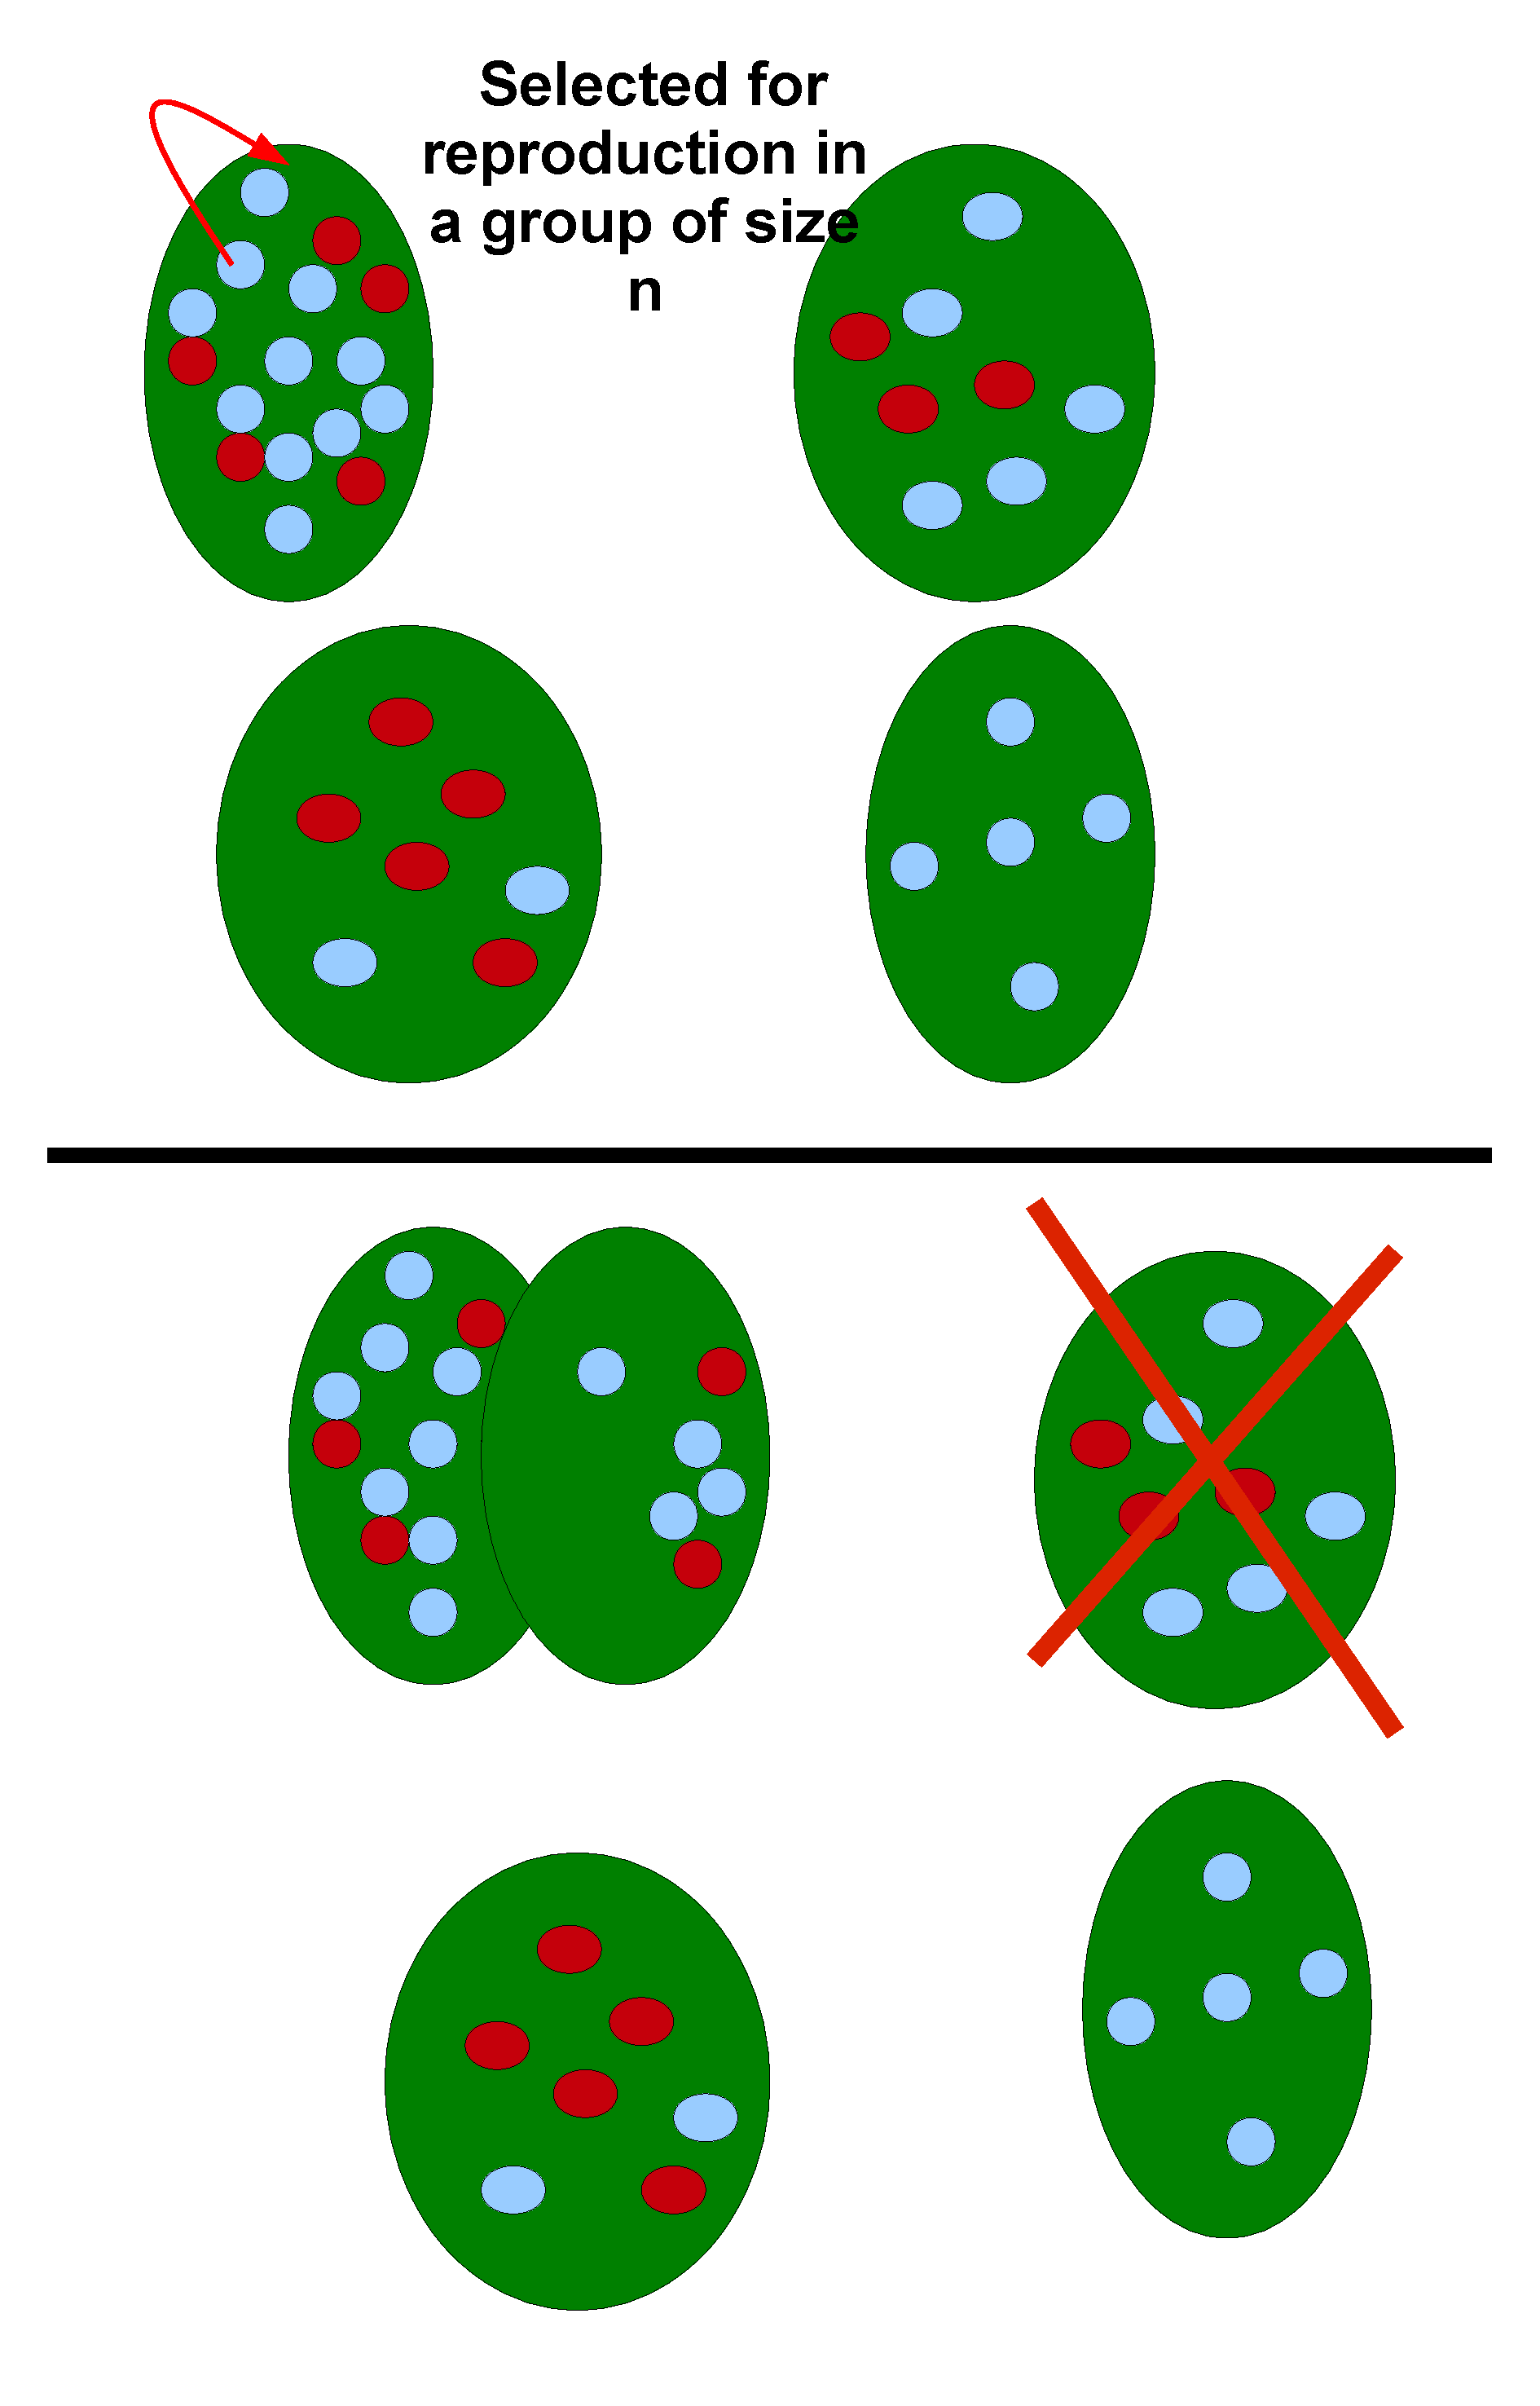
\includegraphics[width=2.5in]{GroupSelection1.pdf} &
b)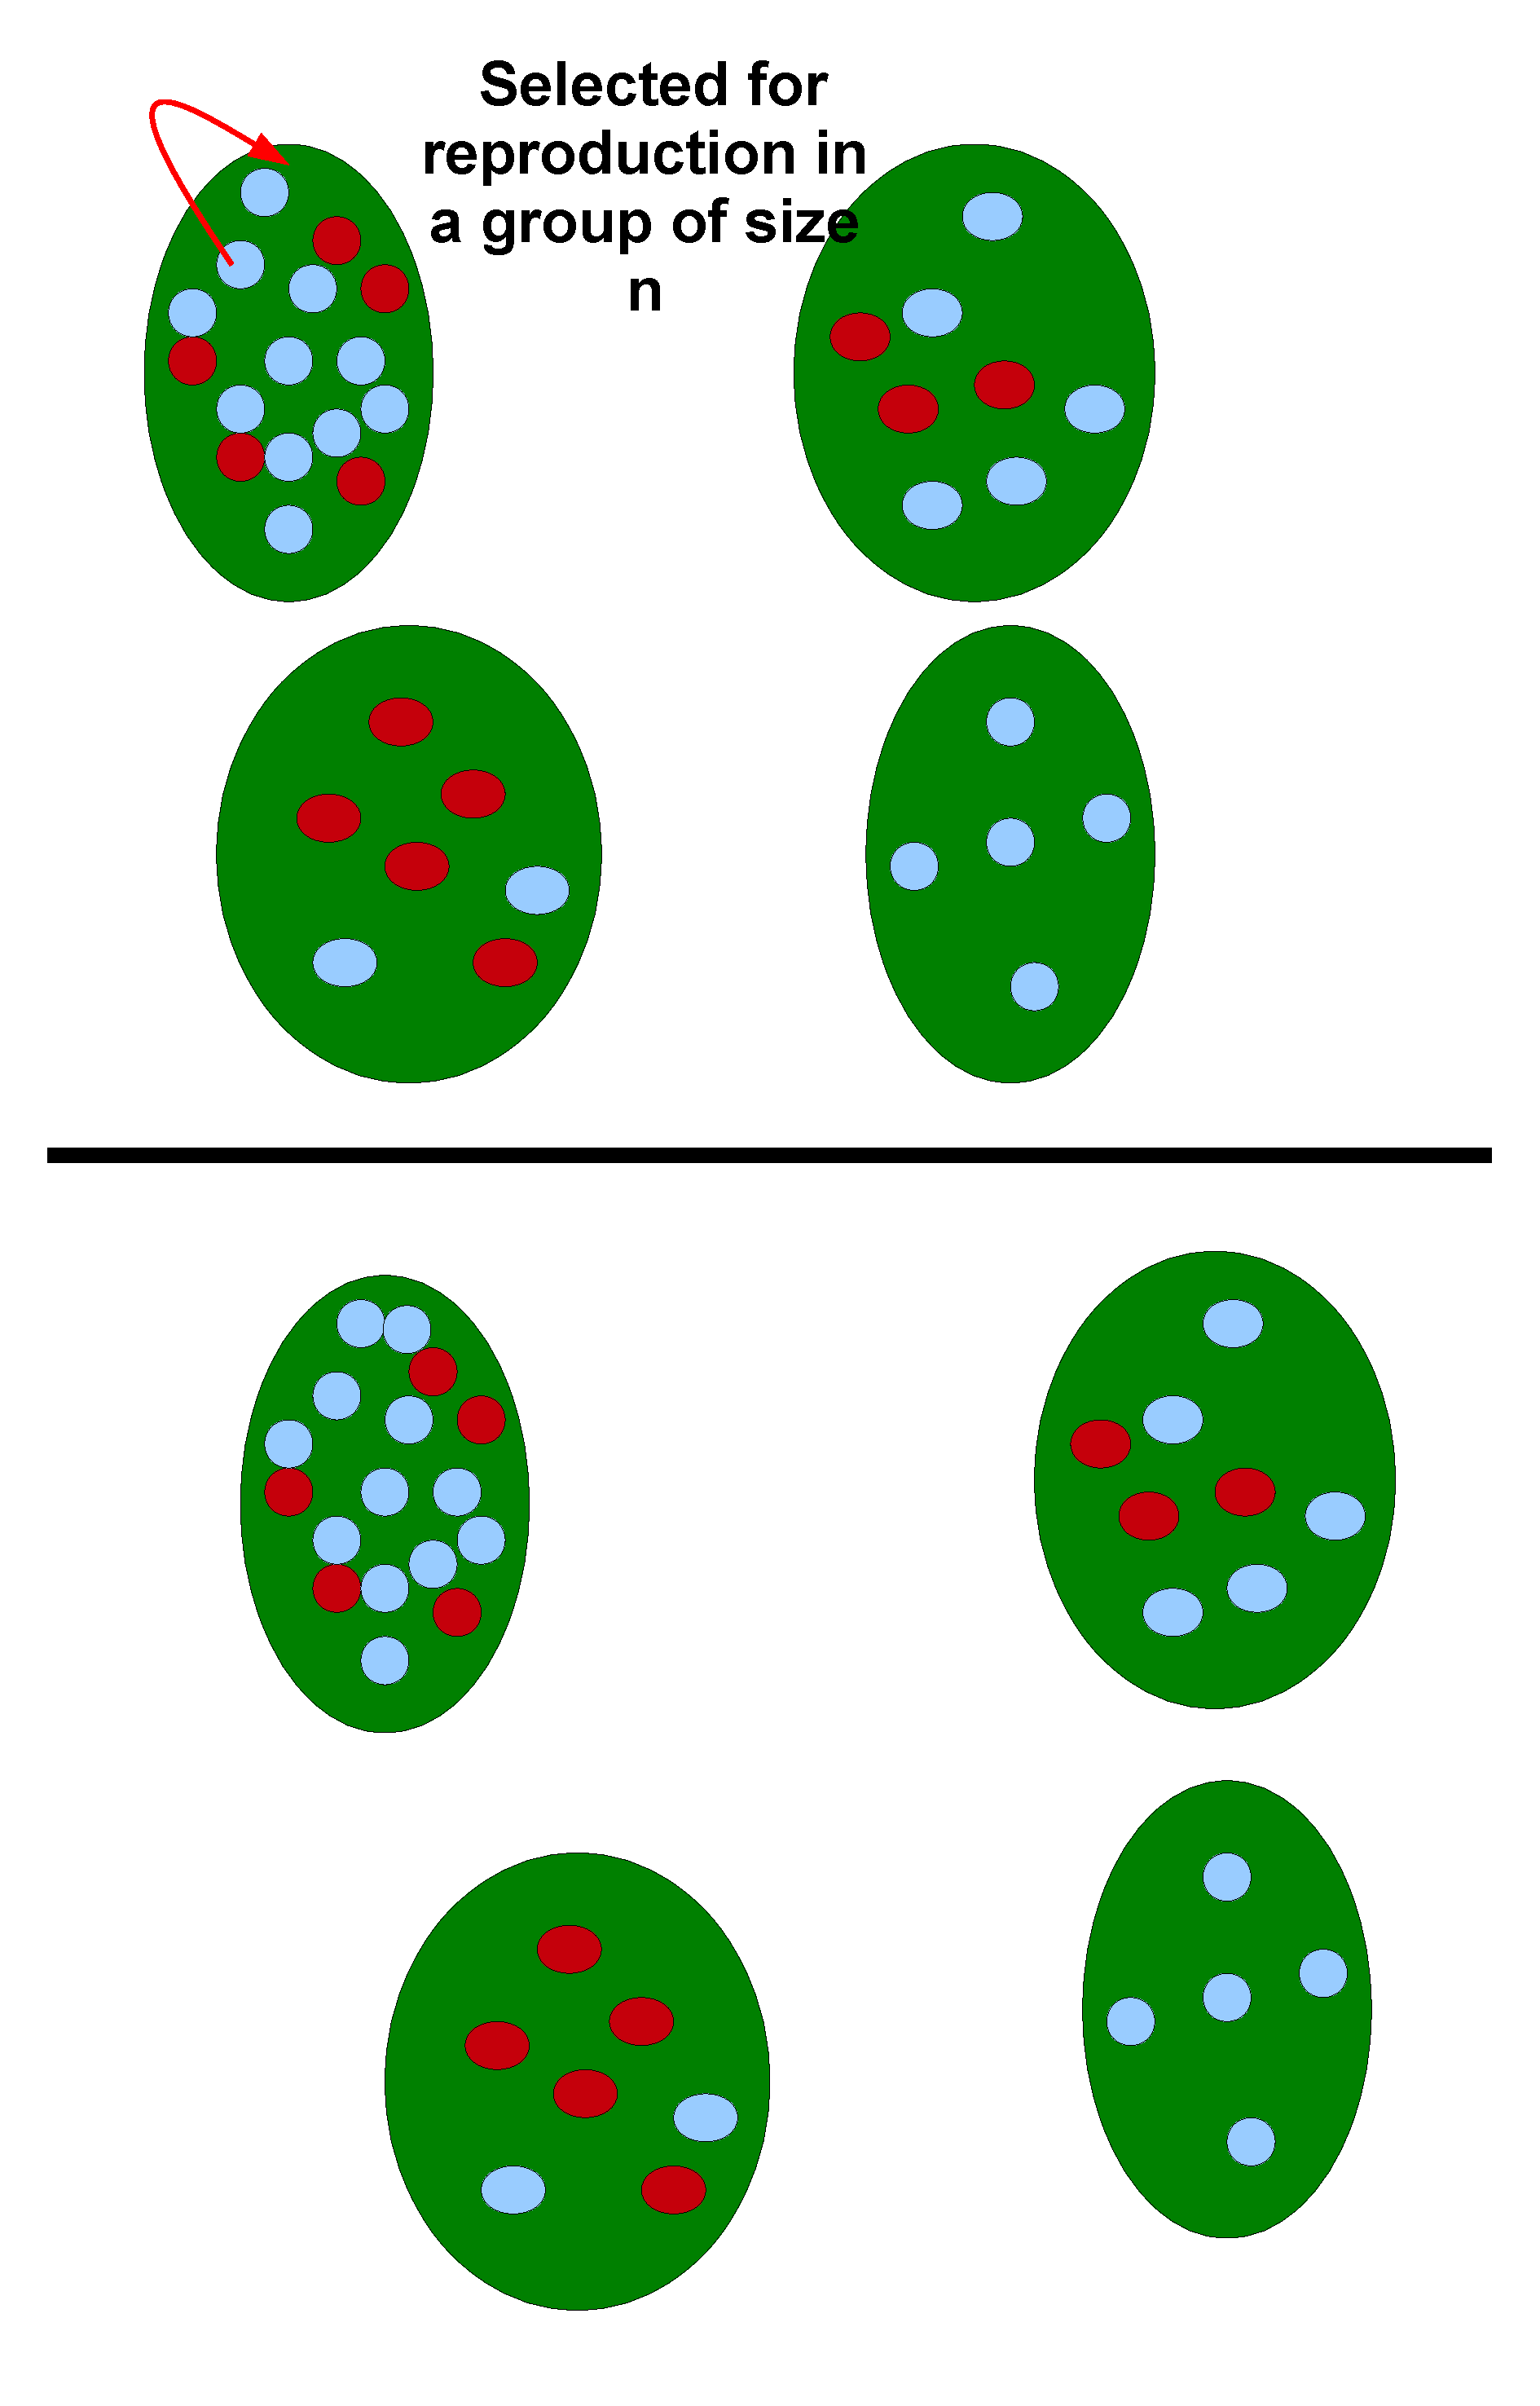
\includegraphics[width=2.5in]{GroupSelection2.pdf}
\end{array}$
\end{center}
\caption{a) . With probability $q$ the group splits in two groups, where generally $q\ll 1$ to allow invasion in groups before any splitting. b) With probability $1-q$ the new offspring take the place of other individual in the group.}
\label{Fig5.2}
\end{figure}

 Fixation probability in group selection is often calculated for an initial single mutant in whole population of $m$ groups of size $n$, with a small $q$\cite{Shoresh2011,Traulsen2006a}. If the splitting probability is small enough, such that the average time for an splitting event is larger than that for fixation of a single mutant in a groups, the fixation probability $\Phi(1)$ in population can be separated in two events: fixation probability $\rho(1,n)$ of a mutant in a group of size $n$, and    fixation probability $\phi(1,m)$ of a single group of mutants in a population of $m$ groups. Thus the risk of dominance of a single mutant is
\begin{equation}
\Phi_1(n,m)=\phi_1(m)\rho_1(n).
\end{equation}
The general form of $\rho_1$ has been already determined in Eq. \eqref{5.14}. A general form for $\phi_1(m)$ can be derived because of the small $q$.
After a mutant of type $A$ has invaded its host group of $n-1$ type $B$ individuals, then the population will be composed  of homogenous groups of $A$ or $B$ individuals. As a result, the transition probability $P_{l,l+1}$ that population changes from $l$ $A$ groups to $l+1$ is the product  of three events:
\begin{itemize}
\item The probability that an individual of type $A$ is selected for reproduction. 
\begin{equation}
\frac{f_A(n)ln}{f_A(n)ln+f_B(0)(l-m)n}.
\end{equation}
\item The probability of splitting $q$
\item The probability that a $B$ group is chosen for elimination.
\begin{equation}
\frac{m-l}{m}
\end{equation}
\end{itemize}
Thus $P_{l,l+1}$ is given by
\begin{equation}
P_{l,l+1}=q\frac{f_A(n)l}{f_A(n)l+f_B(0)(l-m)}\frac{m-l}{m},
\end{equation}
and  $P_{l,l-1}$ by
\begin{equation}
P_{l,l-1}=q\frac{f_B(n)(m-l)}{f_A(n)l+f_B(0)(l-m)}\frac{l}{m},
\end{equation}
In this phase of the process where there are only  homogeneous groups, each group behaves as an individual of fitness $f_{A,B}(n)n$. Consequently the fixation probability of a single mutant of type $A$ in a group has the same form as Eq. \eqref{5.14} for a single mutant in a population of size $m$: 
\begin{equation}\label{5.37}
\phi_{1}(m)=\left(1+ \sum\limits_{k=1}^{m-1}\prod\limits_{l=1}^{k}\frac{f_{B}(0)}{f_{A}(n)}\right)^{-1}
\end{equation} 
Hence, the fixation probability of a single mutant $A$ in a structured population of $m$ groups of maximum size $n$ is given by
\begin{equation}
\Phi_1(n,m)=\left(1+\sum\limits_{k=1}^{n-1}\prod\limits_{j=1}^{k}\frac{f_{B}(j)}{f_{A}(j)}\right)^{-1}\left(1+ \sum\limits_{k=1}^{m-1}\prod\limits_{l=1}^{k}\frac{f_{B}(0)}{f_{A}(n)}\right)^{-1}.
\end{equation} 
In random drift, where a mutant $A$ of fitness $r$ is introduced in a population of $nm-1$ type $B$ individuals with fitness $s$, the respective fixation probability ha an analytical solution, and reduces to   
\begin{equation}
\Phi_1(n,m)=\frac{1-s/r}{1-(s/r)^{n}}\frac{1-s/r}{1-(s/r)^{m}}.
\end{equation}
This is can be corroborated with the stochastic simulation data in (Figure \ref{Fig5.3}).

From this expression  some important features of a structured population can be seen\cite{Traulsen2005}. Comparing the fixation probability $\rho_{1}(r,nm)$ of a single mutant $A$ in a unstructured population of size $nm$ with that for group selection, $\Phi_{1}(r,n,m)$, we see that  for $s<r$ we have $\Phi_{r,n,m}\leqslant \rho_1(r,nm)$, which means that an advantageous mutant is  less likely to be fixated in a structured population. In contrast, for $r<s$ we have $\Phi_{r,n,m}\geqslant \rho_1(r,nm)$, which means that a disadvantageous mutant is more likely to fixate in a structured population. This  shows that the process of group splitting works as a suppressor of individual selection.
 
\begin{figure}[H]\label{Fig5.3}
        \begin{center}
  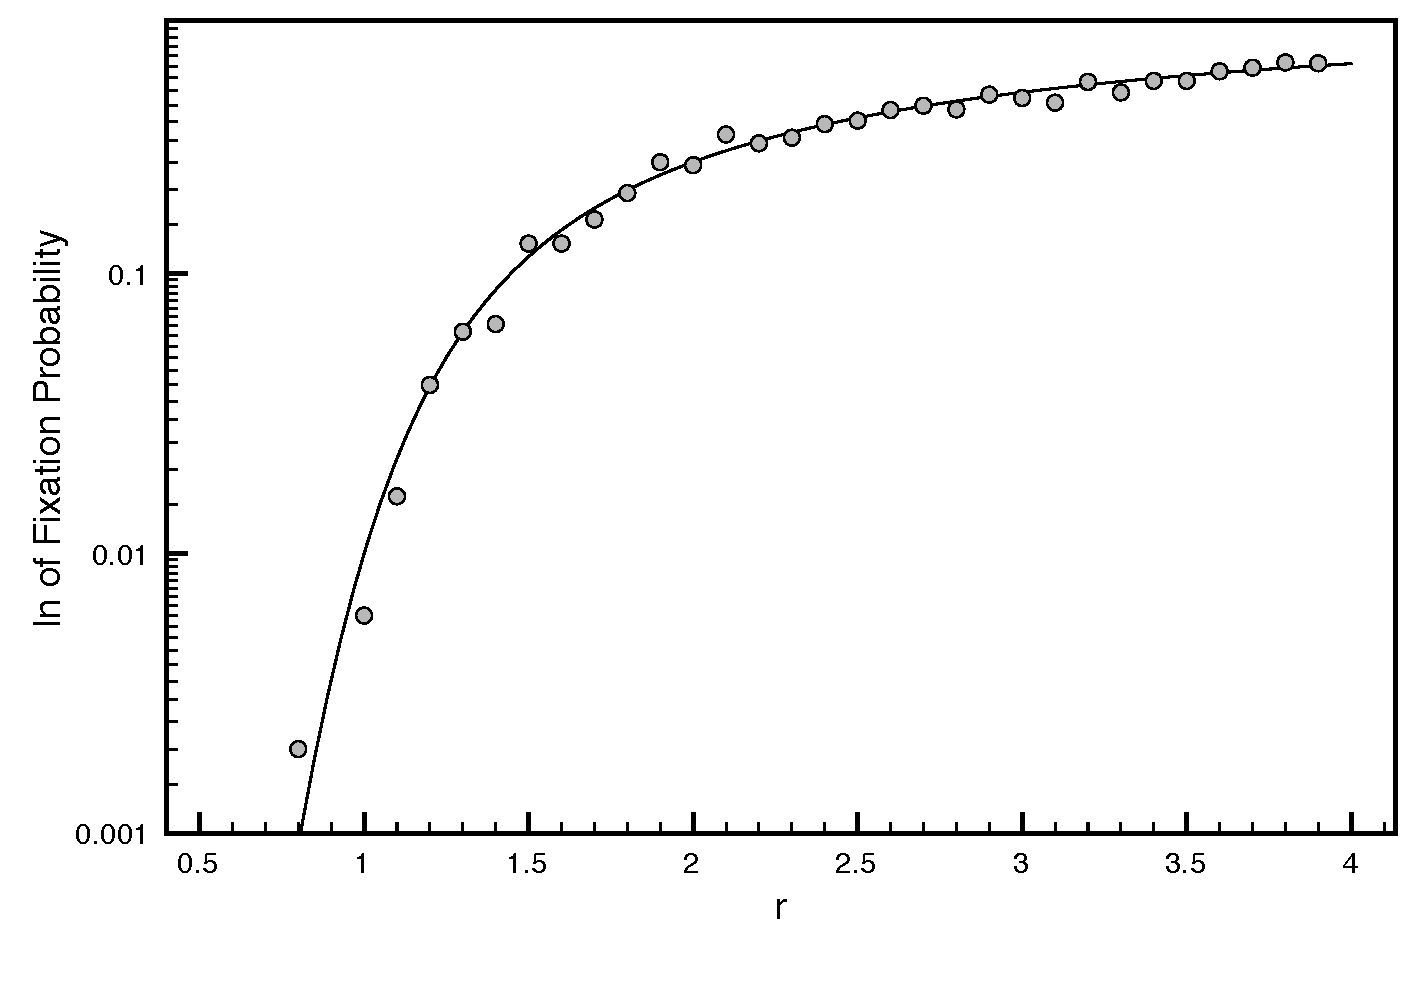
\includegraphics[width=11cm,height=8cm]{m10n10q0001.pdf}
     \end{center}
      \caption{Group selection for no interaction games. $n=10$, $m=10$ and $q=0.001$} 
   \end{figure}
 Now we will study the case of interaction games, where there are social interactions among the individuals of each group. In this system we have type $C$(cooperators) individuals and type $D$(defectors), with the payoff matrix.
 \begin{equation}
 \bordermatrix{~ & C & D \cr
             C & R & S \cr
              D & T & P \cr} 
 \end{equation} 
 and expected fitness by individual
  \begin{equation}
  f_{C}(i)=1-w+w\pi_{C}(i) \;\;\;  f_{D}(i)=1-w+w\pi_{D}(i)
  \end{equation}
 The fixation probability for a single cooperator in a group of $n-1$ defectors, for weak selection, has been already determined in Eq. \eqref{5.29}. Thus
 \begin{equation}
 \rho_{D}(n)=\frac{1}{n} -\frac{w}{6n}\left[ (T-R+2P-2S)n-(T+2R-4P+S)\right].
 \end{equation}
Fixation probability $\phi_{C}(m)$ of a single group of cooperators can be compute using Eq. \eqref{5.37}, which for weak selection is\cite{Traulsen2006a}
\begin{equation}
\phi_{D}(m)=\frac{1}{m}\left[1+\frac{w}{2}(m-1)(R-P)\right].
\end{equation} 
Therefore the fixation probability of a single mutant in a structure population of $m$ groups of size $n$ is given by
\begin{equation}
\Phi_{C}(n,m)=\frac{1}{mn}\left[1+w\left(-\frac{(T-R+2P-2S)n-(T-4R+2P+S)}{6}+\frac{m-1}{2}(R-P)\right)\right].
\end{equation}
Using Eq. \eqref{5.31} for a single defector in a group, and the fixation probability of a single defector group,
\begin{equation}
\phi_{D}(m)=\frac{1}{m}\left[1-\frac{w}{2}(m-1)(R-P)\right],
\end{equation}
the fixation probability of a single defector in structured population is
\begin{equation}
\Phi_{D}()n,m)=\frac{1}{nm}\left[1+w\left(\frac{1}{6}((2T-2R+P-S)n-(T-4R+2P+S)) +\frac{m-1}{2}(R-P)\right)\right].
\end{equation}
Now let us compare these analytical approximations with the pair interaction stochastic simulation. For this propose  a prisoner's dilemma  game will be used,  with the payoff matrix
\begin{equation}
\bordermatrix{~ & C & D \cr
             C & b-c & -c \cr
              D & b & 0 \cr},
\end{equation}
where $c$ represents the cost of cooperating and $b$ the benefit that an individual gets from the cooperation of its partner. In (Figure \ref{Fig5.4})  the population fraction as a function of time steps for group selection is shown, where the peaks represents the splitting of a group, the division of a group of size $n$ replaces another group of size $n$ most likely by a new group of $n/2$ individuals, which explains the abrupt changes in population.     
\begin{figure}[H]\label{Fig5.4}
        \begin{center}
  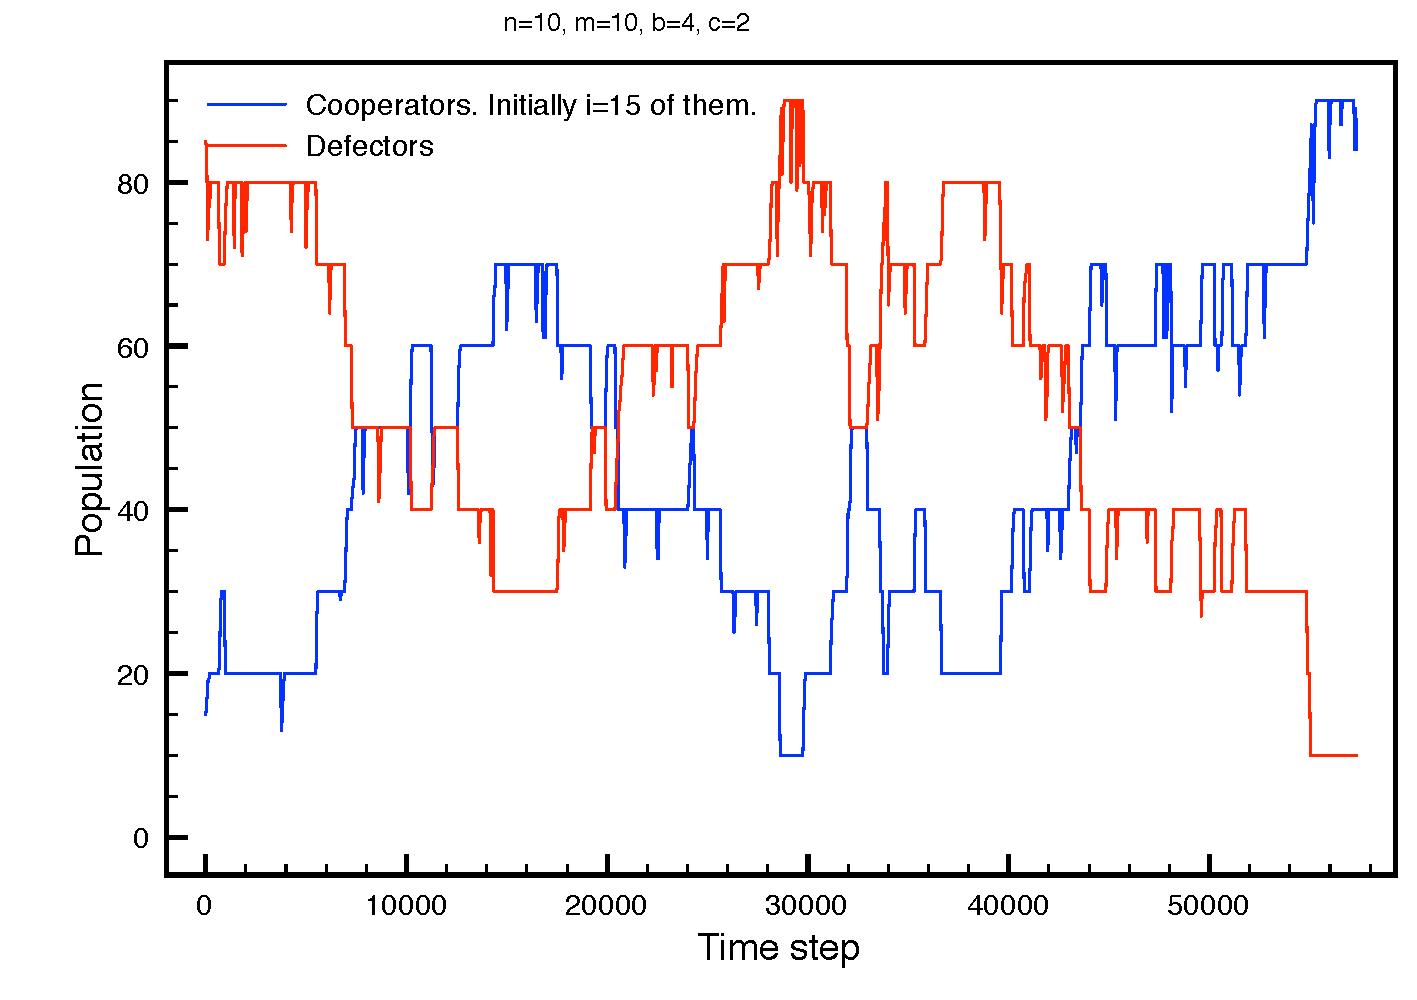
\includegraphics[width=11cm,height=8cm]{groupselection.pdf}
     \end{center}
      \caption{The peaks are the splitting of a group. $q=0.001$} 
   \end{figure}
Now let us analyze the conditions where a cooperator is more likely to invade a structure population of defectors than a single defector invade  a population of cooperators. In other words, what are the values of the ratio $c/b$ where $\Phi_{C}(n,m)\geq \Phi_{D}(n,m)$. For $b$ and $c$, the fixation probabilities simplify to
\begin{equation}
\Phi_{C}(n,m)=\frac{1}{mn}\left[1+w\left(-\frac{1}{6}(3cn+3(c-b))+\frac{m-1}{2}(b-c)\right)\right] 
\end{equation}
\begin{equation}
\Phi_{D}(n,m)=\frac{1}{mn}\left[1+w\left(\frac{1}{6}(3cn+3(c-b))-\frac{m-1}{2}(b-c)\right)\right].
\end{equation}
The inequality reduces to
\begin{equation}
(m-1)(b-c)\geq cn + c-b ,
\end{equation}
which can be written as
\begin{equation}
\frac{b}{c}\geq \frac{n}{m-2} + 1.
\end{equation}
From this inequality it is inferred  that the benefit to cost ratio where a cooperator is most likely to invade than a defector, depends on the structure of population. This inequality is compared in the next figure with data obtained from a group selection simulation for different values of $m$ (Figure \ref{}).
\begin{figure}[H]\label{}
        \begin{center}
  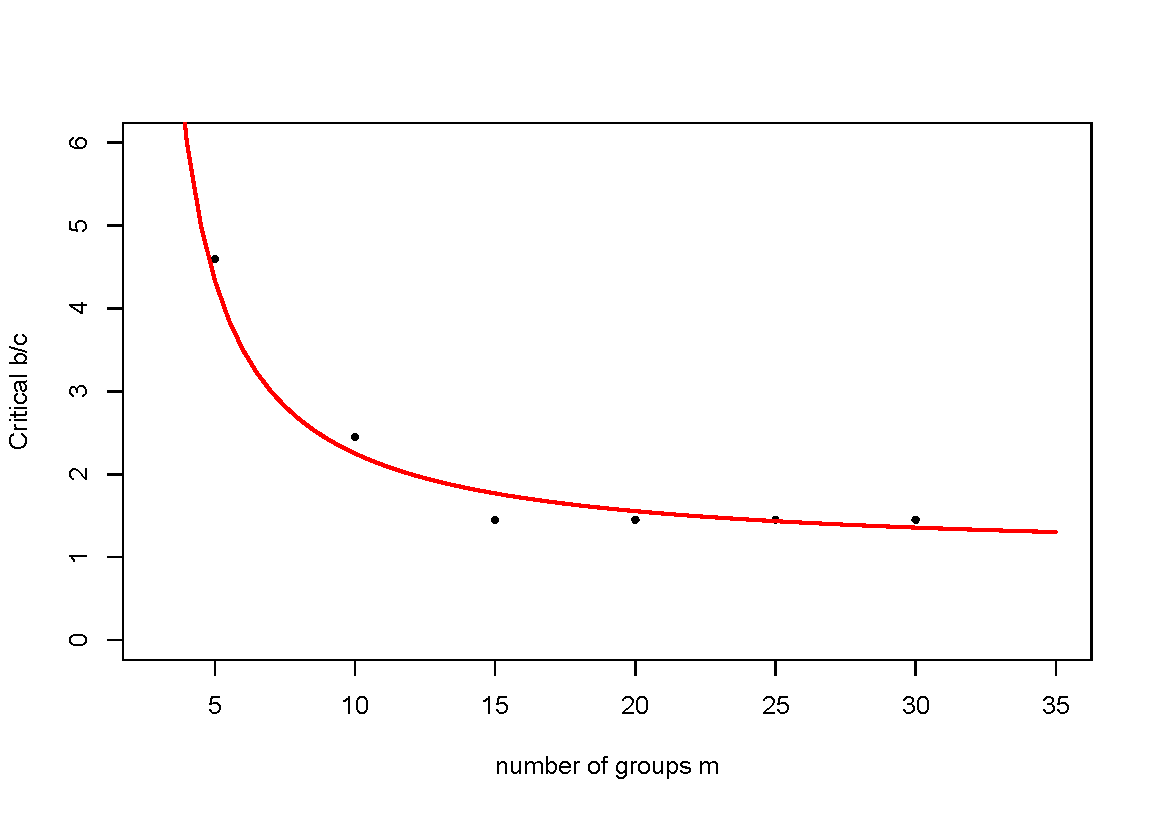
\includegraphics[width=11cm,height=8cm]{bcratio.pdf}
     \end{center}
      \caption{Group selection curve for invasion, $q=0.001$, $w=0.1$ and $n=10$.} 
   \end{figure}
%%% Local Variables: 
%%% mode: latex
%%% TeX-master: "../thesis"
%%% End: 

%%% Thesis Introduction --------------------------------------------------
\chapter{From Stochastic Equations to Deterministic Average Equations}
\ifpdf
    \graphicspath{{FromStochastic/Figs/PNG/}{FromStochastic/Figs/PDF/}{Fromstochastic/Figs/}}
\else
    \graphicspath{{FromStochastic/Figs/EPS/}{FromStochastic/Figs/}}
\fi
In the literature we find differential equations for growth  processes, such as: protein production and degradation, predator-prey dynamics such as the Lolka-Volterra equations and selection dynamics as Eq. \eqref{3.12}. These are deterministic descriptions of those processes, which really are stochastic. What these equations are telling us is about the average behavior of those systems, but how can those equations be derived from the master equation Eq. \eqref{4.1}? Many of these differential equations have been proposed without a direct explanation of their relation with the implicit stochastic process \cite{Traulsen2005a}. For example, the equation 
\begin{equation}\label{6.1}
\frac{dx_i}{dt}=x_i(\pi_i(x) - \bar\pi)
\end{equation}  
for replication dynamics in evolutionary game theory is not the result from averaging over the master equation of its respective Moran process. This also happens with random drift and Eq. \eqref{3.12}, where the average of the stochastic simulation does not fit with the solution of this equation.  

In this section  a simple approach to derive the average differential of some simple stochastic systems will be shown, such as that of protein creation and degradation and for more difficult master equation as those that result in Moran process for evolutionary dynamics, using Focker-Planck approximation and Langevin equation.
\section{A Simple Example: Protein creation and degradation}
Inside any cell there is a genetic system that is  responsible for the production of the proteins that the cell needs. Suppose that the expression rate of protein is $\gamma$, but inside of cell this proteins also have a degradation, that can be represented by the rate $\beta$. Because of the stochasticity these rates represents the probabilities by unit time of creation or degradation.
Taking $1$ as the time step and assuming it is small enough compared to $\gamma$ and $\beta$ that just one events happens at each time step\cite{Pedraza1,Thattai},  the master equation  for the state of $i$ proteins is
\begin{equation}\label{6.2}
\frac{dp_i(t)}{dt}=-(\gamma + i\beta)p_i(t) + (i+1)\beta p_{i+1}(t) + \gamma p_{i-1}(t).
\end{equation} 
where $i$ goes from $0$ to $\infty$ and the average of $i$ is represented by
\begin{equation}
\langle i\rangle=\sum\limits_{i=0}^{i=\infty}ip_i (t).
\end{equation}
Averaging over Eq. \eqref{6.2} we get
\begin{equation}
\frac{d \langle i\rangle}{dt}=-\sum\limits_{i=0}^{i=\infty}i(\gamma + i\beta)p_i(t) + \sum\limits_{i=0}^{i=\infty}i(i+1)\beta p_{i+1}(t) + \sum\limits_{i=0}^{i=\infty}i \gamma p_{i-1}(t).
\end{equation}
and replacing the next summations in the above equation
\begin{equation}
\sum\limits_{i=0}^{\infty}i\gamma p_{i-1}(t)=\sum\limits_{i=0}^{\infty}(i+1)\gamma p_{i}(t)\;\;\; 	\sum\limits_{i=0}^{\infty}i(i+1)\beta p_{i+1}(t)
\end{equation} 
the average  simplifies to the differential equation
\begin{equation}
\frac{d \langle i\rangle}{dt} = \gamma - \beta \langle i \rangle.
\end{equation}
Which has the solution
\begin{equation}
\langle i \rangle =\frac{\gamma}{\beta}+\left(\langle i\rangle_0 -\frac{\gamma}{\beta}\right)e^{-\beta t}
\end{equation}
and the average protein number $\langle i\rangle=\gamma/\beta$ in steady state.

We can also determine the steady state protein distribution by taking $\frac{dp_i(t)}{dt}=0$ in the master equation
\begin{equation}
0=-(\gamma + i\beta)p_i(t) + (i+1)\beta p_{i+1}(t) + \gamma p_{i-1}(t),
\end{equation}
which can be written as
\begin{equation}
(i+1)p_{i+1}-\langle i\rangle p_i = i p_i - \langle i \rangle p_{i-1}.
\end{equation} 
 Setting $y_i=i p_i - \langle i \rangle p_{i-1}$ and using the above equation, the sum over $y_i$ is
\begin{equation}
\sum\limits_{i=0}^{\infty}y_i =0.
\end{equation} 
Then $y_i$ must be $0$, and the recurrence equation for $p_i$ is
\begin{equation}
p_i = \frac{\langle i \rangle}{i} p_{i-1}
\end{equation}
Therefore
\begin{equation}
p_i=\frac{\langle i\rangle^i}{i!}p_0.
\end{equation}
Because of $\sum\limits_{i=0}^{\infty}p_i=1$ and $\sum\langle i \rangle^i / i!=e^{\langle i \rangle}$, $p_0=e^{\langle i \rangle}$ and finally
\begin{equation}
p_i =\frac{\langle i \rangle ^i}{i!}e^{-\langle i\rangle}.
\end{equation}
 The steady state of proteins have a Poisson distribution, which for large $\langle i \rangle$ can be approximated to a continuos Gaussian distribution.
   
These two results; the deterministic law and steady state distribution, were simple to determinate due to the lineal form of the transition rates $P_{i,i+1}$ and $P_{i,i-1}$ of this system; but even then, the dynamical distribution is difficult to calculate analytically. Next we will see some approximation methods to calculate the deterministic law when the transition probabilities are not lineal.  
\section{Average Differential Equations in Evolutionary Dynamics}
In this section  an approximation method to find deterministic differential equations from stochastic systems, where the transition probabilities are non-linear functions of the stochastic state variable $i$, will be explained.  

In evolutionary dynamics we have transition probabilities that are not linear function of the population frequency $i$, which have the form
\begin{equation}
P_{i,i+1}=\frac{1-w+w\pi_C}{1-w+w\langle \pi \rangle}\frac{i}{n}\frac{n-i}{n}\;\;\; P_{i,i-1}=\frac{1-w+w\pi_D}{1-w+w\langle \pi \rangle}\frac{i}{n}\frac{n-i}{n}.
\end{equation}
Introducing these transitions into the  master equation  
\begin{equation}
\frac{d P_{i}(t)}{dt}=-(P_{i,i+1} + P_{i.i-1})P_{i}(t) + P_{i+1,i}P_{i+1}(t)+ P_{i-1,i}P_{i-1}(t),
\end{equation}
and averaging over all the systems we will find terms of the form
\begin{equation}
\sum\limits_{i=0}^{n}\frac{1-w+w\pi(i)_C}{1-w+w\langle \pi(i) \rangle}\frac{i}{n}\frac{n-i}{n} i P_{i}(t),
\end{equation}
which need to be transformed to get averages of $i$, and write the average differential equation as
\begin{equation}
\frac{d\langle i \rangle}{dt}=f(\langle i \rangle,\langle i \rangle^2, .., \langle i \rangle^m).
\end{equation}  
This method to obtain the deterministic law is difficult. However it is possible to use a easier method using the relation between Fokker-Planck equation and Langevin equation.

 
First, to determine the Fokker -Planck equation, let us set $P_{i,i+1}=P_{i}^{+}$ and $P_{i,i-1}=P_{i}^{-}$, and consider the case where $i$ is large and behaves as a continuos variable. We can then write the transition probabilities as
\begin{equation}
P_{i}^{+}=P^{+}(i)\;\;\; and \;\;\; P_{i}^{-}=P^{-}(i).
\end{equation}  
Expanding the terms $P(i\pm 1,t)$, $P^{+}(i\pm1)$ and $P^{-}(i\pm1)$ as a Taylor series up to second order, the Fokker-Planck equation for the Moran process(one step process) is\cite{Traulsen2005a}
\begin{equation}\label{6.19}
\frac{\partial P(i,t)}{\partial t}=-\frac{\partial}{\partial i}\left[\left(P^{+}(i)-P^{-}(i)\right)P(i,t)-\frac{1}{2}\frac{\partial}{\partial i}\left(P^{+}(i)+P^{-}(i)\right)P(i,t)\right].
\end{equation} 
This equation is often used to calculate the probability distribution and averages in steady state. This can also be done with the Langevin approach.

Langevin proposed an stochastic differential equation of the form
\begin{equation}\label{6.20}
\frac{di}{dt}=a(i,t) + b(i,t)\xi(t),
\end{equation}
that have a deterministic part $a(i,t)$ and the stochastic $b(i,t)\xi(t)$, where $\xi(t)$ is an uncorrelated time random variable with white noise $\langle\xi\rangle=0$. Since this is a Langevin approach for the Moran process, the quantities $a(i,t)$ and $b(i,t)$ must  satisfy the absorbing states $0$ and $n$, where $di/dt=0$. Therefore $a(i,t)=0$ and $b(i,t)=0$ for $i=0,n$. This tells us that these factors have a relation with the transition probabilities.

Ito's calculus lets us establish the equivalence between Langevin and Fokker-Plank\cite{Kampen, Gardiner}. For an  arbitrary function $f[i(t)]$,  Ito's formula for the expansion of the differential $df[i(t)]=f[i(t)+di(t)]-f[i(t)]$ is
\begin{equation}
df[i(t)]=\{a(i,t)\partial_{i}f+\frac{1}{2}b^2(i,t)\partial_{i}^{2}f\}dt+b(i,t)\partial_{i}f\xi dt.
\end{equation}  
Averaging this equation
\begin{equation}
\frac{d}{dt}\langle f[i(t)]\rangle=\langle a(i,t)\partial_{i}f+\frac{1}{2}b^2(i,t)\partial_{i}^{2}f\rangle + \langle b(i,t)\partial_{i}f\xi\rangle,
\end{equation}
where because of the irregularity of $\xi$, $\langle b(i,t)\partial_{i}f\xi\rangle=0$. Thus
\begin{equation}
\int f(i) \partial_{t}P(i,t) di=\int a(i,t)\partial_{i}f P(i,t) di +\int\frac{1}{2}b^2(i,t)\partial^{2}_{i}f P(i,t)di .
\end{equation}
 Integrating by parts this becomes
 \begin{equation}
 \int f \partial_{t}Pdi=aPf\mid-\int\partial_{i}(aP)fdi + \frac{1}{2}b^{2}P\partial_{i}f\mid -\int\frac{1}{2}\partial_{i}(b^2P)\partial_{i}f di 
 \end{equation} 
 and once again for the integral that contains $\partial_{i}f$
 \begin{equation}
  \int f \partial_{t}Pdi=aPf\mid-\int\partial_{i}(aP)fdi + \frac{1}{2}b^{2}P\partial_{i}f\mid - \frac{1}{2}\partial_{i}(b^2P)f\mid + \int\frac{1}{2}\partial^{2}_{i}(b^2P)fdi,
 \end{equation}  
  where the boundary terms banish because they  are evaluated in the absorbing states $i=0,n$. Therefore we obtain
  \begin{equation}
  \int \partial_{t}P f di=\int\left( -\partial_{i}(aP)+\frac{1}{2}\partial^{2}_{i}(b^2P)\right)fdi.
  \end{equation} 
 Since $f(i)$ is arbitrary, the integral terms correspond to Fokker-Planck equation
 \begin{equation}\label{6.27}
 \partial_{t}P(i,t)= -\partial_{i}(a(i,t)P(i,t))+\frac{1}{2}\partial^{2}_{i}(b^2(i,t)P(i,t)).
 \end{equation}  
 Notice that $f(i)$ can be $i(t)$. Then the Langevin equation
 \begin{equation}
 \frac{di}{dt}=a(i,t) + b(i,t)\xi(t)
 \end{equation} 
 is equivalent to Fokker-Planck Eq. \eqref{6.27}. Therfore by similitude  with Eq. \eqref{6.19}, the coefficients $a(i,t)$ and $b(i,t)$ are written in terms of transition probabilities as
 \begin{equation}
 a(i)=P^{+}(i)-P^{-}(i)\;\;\; , \;\;\; b(i)=\sqrt{P^{+}(i)+P^{-}(i)}.
 \end{equation} 
Hence, the result of the Langevin approach  is the macroscopic equation plus a noise term; the macroscopic(deterministic) or average differential equation is
\begin{equation}
\frac{d\langle i\rangle}{dt}=P^{+}(\langle i\rangle)-P^{-}(\langle i\rangle)\;\;\; for\;\;i\gg1\;\;\; or \;\;\; \mid i-\langle i\rangle\mid\ll 1.
\end{equation} 
Now let us see the evolutionary dynamics differential equation. Setting $x=i/n$ and taking in to account that $n\gg 1$ we obtain
\begin{equation}
\frac{dx}{dt}=\frac{x}{n}\frac{\pi_{C}(x)-\langle\pi(x)\rangle}{\Gamma+ \langle\pi(x)\rangle}.
\end{equation}
Where $\pi_{C}(x)=R(x-1/n)+S(1-x)$,  $\langle\pi(x)\rangle=\pi_{C}(x)x +\pi_{D}(x)(1-x)$ and $\Gamma=(1-w)/w$. For $w=1$ this equation has the term $ \langle\pi(x)\rangle$ unlike the standard replicator Eq. \eqref{6.1}. From this it is good 
to point out that there are different types of transition probabilities for the Moran process, such as Fermi imitation and local update mechanism\cite{Traulsen2009}.
Using the payoff matrix Eq. \eqref{5.1} and its respective elements for random drift, the macroscopic equation for random drift is
\begin{equation}\label{6.32}
\frac{dx}{dt}=\frac{x}{n}\frac{(1-x)(r-s)}{xr+s(1-x)}.
\end{equation}
Below in Figure (\ref{Fig6.1}) simulations of random drift and a comparison with the standard replication equation Eq. \eqref{3.12} for large populations are shown , where a considerable difference is observed .  

\begin{figure}[H]
\begin{center}$
\begin{array}{cc}
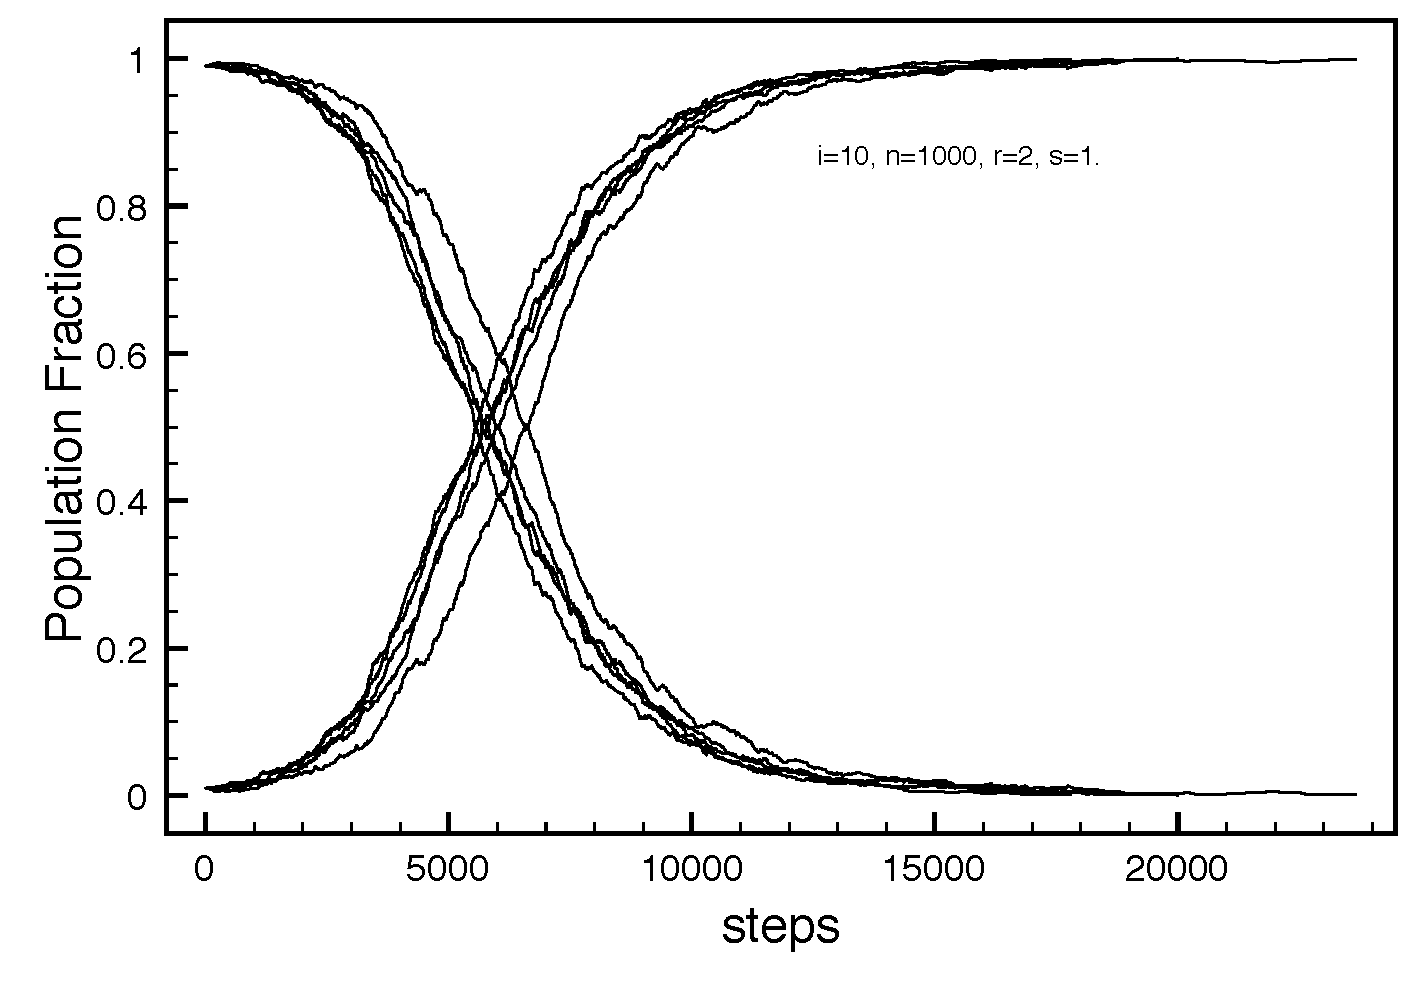
\includegraphics[width=2.5in]{RandomDriftSimulations5.pdf} &
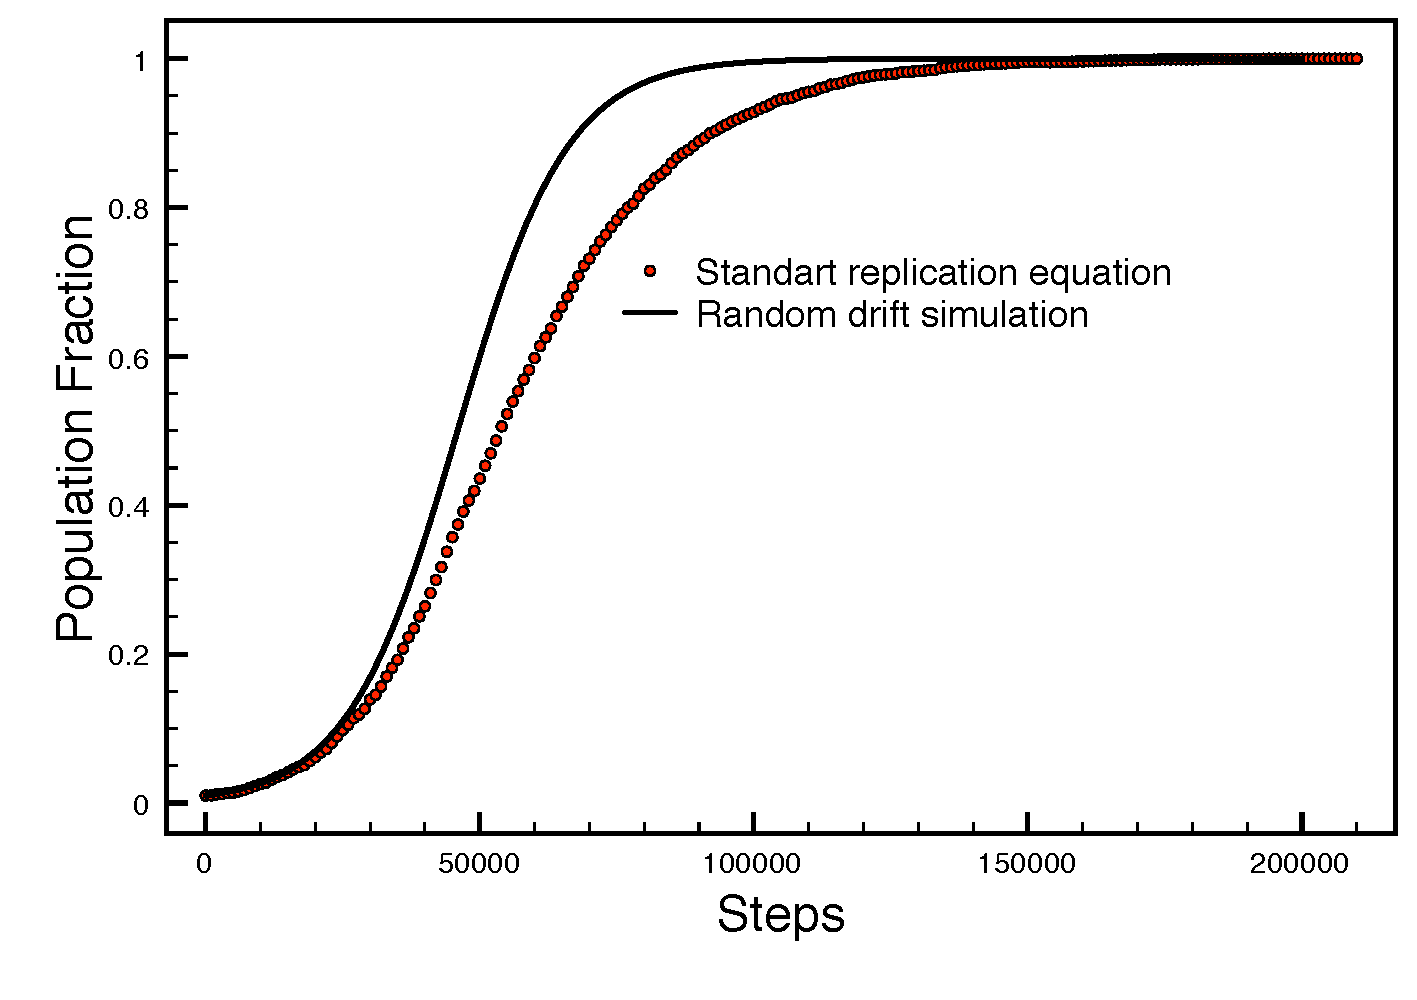
\includegraphics[width=2.5in]{SelectionVsRandom.pdf}
\end{array}$
\end{center}
\caption{Left: Five simulations of random drift for a no so large population $n=1000$. Right: Comparison of random drift and standard replication dynamics(with $t=t' 10000$) for a population of $10000$ and an initial state of $100$ individuals with fitness $r=2$. The other type with $s=1$.}
\label{Fig6.1}
\end{figure}
  
In  Figure \ref{Fig6.2} it is shown how a stochastic simulation for large $n$ population size is close to the deterministic solution of  Eq. \eqref{6.32}, which satisfies the  law of large numbers in stochastic processes.  

  \begin{figure}[H]
  \begin{center}
    \leavevmode
    \ifpdf
      \includegraphics[width=9cm,height=8cm]{DifferentialEquationVsStochastic.pdf}
    \else
      \includegraphics[width=9cm, height=8cm]{DifferentialEquationVsStochastic.pdf}
    \fi
    \caption{In this graph it is shown how the average differential equation fits to a random drift simulation.}
    \label{Fig6.2}
  \end{center}
  \end{figure}

 %%% ----------------------------------------------------------------------

%%% Local Variables: 
%%% mode: latex
%%% TeX-master: "../thesis"
%%% End: 

%%% Thesis Introduction --------------------------------------------------
\chapter{No Deterministic Fitness due to Internal Gene Expression Noise}
\ifpdf
    \graphicspath{{NoDeterministic/Figs/PNG/}{NoDeterministic/Figs/PDF/}{NoDeterministic/Figs/}}
\else
    \graphicspath{{NoDeterministic/Figs/EPS/}{NoDeterministic/Figs/}}
\fi
\markboth{\MakeUppercase{\thechapter. No Deterministic Fitness due to Internal Gene Expression Noise}}{\thechapter. No Deterministic Fitness due to Internal Gene Expression Noise}

Gene expression noise is a consequence of  stochastic variation in cellular processes, such as mRNA transcription an protein synthesis, which are due to extrinsic and intrinsic noise of organisms\cite{Hilfinger2011,Paulsson2004}. These intrinsic stochastic fluctuations results in the variability of isogenic populations of cells under equal environment conditions\cite{Wang2011}. When noise is small, individual cells behaves similar to the average population, but when noise is comparable to the average population, this can have large effects on the macroscopic characteristics of a population of organisms, such as fixation probabilities, average fitness, fixation times and steady-state points\cite{Mettetal2008}.
            
Noise has an important role in biological systems and evolution, it is responsible of adaptive mutations in organism, where new traits in species face in a  successful way adversities in nature that old traits do not. This is a  beneficial result of noise in biological systems, but it also can have deleterious consequences on the optimums performance of phenotypes in organisms.

In the present chapter, first it will be defined which stochastic process are considering extrinsic and intrinsic to individuals in our evolutionary simulation, and how the intrinsic cellular noise affects the fitness of a phenotype. To do this, we present the functional dependence of fitness with protein expression level, which has optimums values. Next, distributions of fitness are introduced into the evolutive simulation, and the resulting macroscopic quantities measured for several values of noise and types of fitness distribution. Finally we compare this results to the fitness deterministic case and create a dynamical   analytical approximation  to relate intrinsic and extrinsic noise.    
\section{Gene Expression Noise in Moran Process}
In this model we have a stochastic process of Moran replication, where two organisms with different characteristics compete in an environment  that is at its maximum resource capacity, and therefore has a finite and constant population size. The stochasticity in  the simulations that have been shown in  previous chapters is due to  factors external to  individuals. For example, fluctuations in  food sources in a media  for growing bacteria, or aleatory changes in temperature, these are the fluctuations that  random numbers simulate in these previous models. However, this model  does not assume that there are  also intrinsic fluctuations in organisms  that are not taken into account at the moment when an individual reproduces. The standard Moran process assumes that the new offspring is an exact copy of its parent, which does not  happen with real organisms due to gene network noise. These fluctuations are due to random births and deaths of molecules in  gene expression dynamics inside organisms. Gene expression is responsible for generating the traits of phenotypes. As a result of this noise, it generates  phenotype variability in isogenic populations. 

The resulting fitness distribution will be added in the simulation at the moment of replication, and the new offspring will have a fitness that comes from this stochastic distribution. Here we assume that each time step in  Moran process is equivalent to the time that organisms as bacteria take to reproduce. In other words we are considering that the protein distribution is the steady state distribution.  

\section{Fitness as a Function of Gene Expression}
We have defined fitness as the reproductive contribution by individual to next generation. This fitness depends on any phenotype of the organisms.It is know, that gene repression or activations generate the lack or accentuation of a phenotype characteristic. This characteristic can lead us intuitively to think that fitness monotonically depends on gene expression level , but this is an incorrect consideration. Instead fitness is a non-monotonic function of gene expression with optimal and critical values.  A way to analyzing this  assumption, is to consider that, if a bacterium expends lots of its energy producing proteins to generate any phenotype, it will not have enough energy for producing biomass, in others words, for replication. In the other hand, if the bacterium has a low expression of the gene corresponding to a phenotype,  this characteristic will not be enough successful, which does not represent a reproductive advantage. 

Protein synthesis is a costly process for organisms, and there should be optimal expression levels for each gene. To compute these optimum levels of protein synthesis, have been proposed  models based in the trade-off between the cost energy and the reproductive(biomass production) benefit of gene expression level\cite{Kahn2010, Wang2011}. These models  shown that, fitness is a limited non-monotonic function of protein synthesis, which means that there is a range where fitness is a non-null positive value with a maximum. In next  (Figure \ref{Fig7.1}), are shown some fitness functions from the works of Kahn and Wang.
\begin{figure}[H]
\begin{center}$
\begin{array}{cc}
a)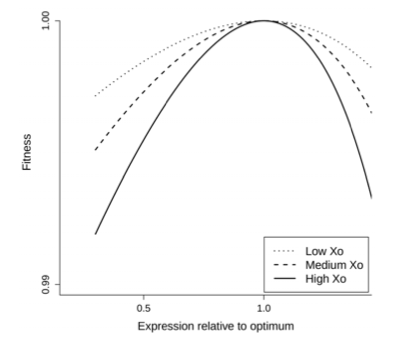
\includegraphics[width=2.5in]{FitnesVsexpression1.png} &
b)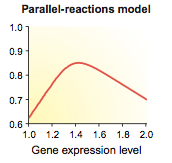
\includegraphics[width=2.5in]{FitnessVsExpression2.png}
\end{array}$
\end{center}
\caption{a): These curves represent the fitness function for different values of the optimal expression level $x_{0}$. They were generated assuming a benefit and cost functions, $B(x)$ and $C(x)$, where the x-axis is the expression level relative to the optimum. This graph was taken from \cite{Kahn2010}  b): Parallel reaction model in a gene metabolic network, where the vertical axis represents fitness. This graph was taken from\cite{Wang2011}.}
\label{Fig7.1}
\end{figure}

The non-monotonic form of fitness functions, leads to special properties when we examine the resulting distribution fitness from a protein distribution. To study these properties, we are going to use a simple triangular fitness function (Figure. \ref{Fig7.2}). With this testing function, we will measure the average fitness for several values of protein  variance.
\begin{figure}[H]
\begin{center}$
\begin{array}{cc}
a)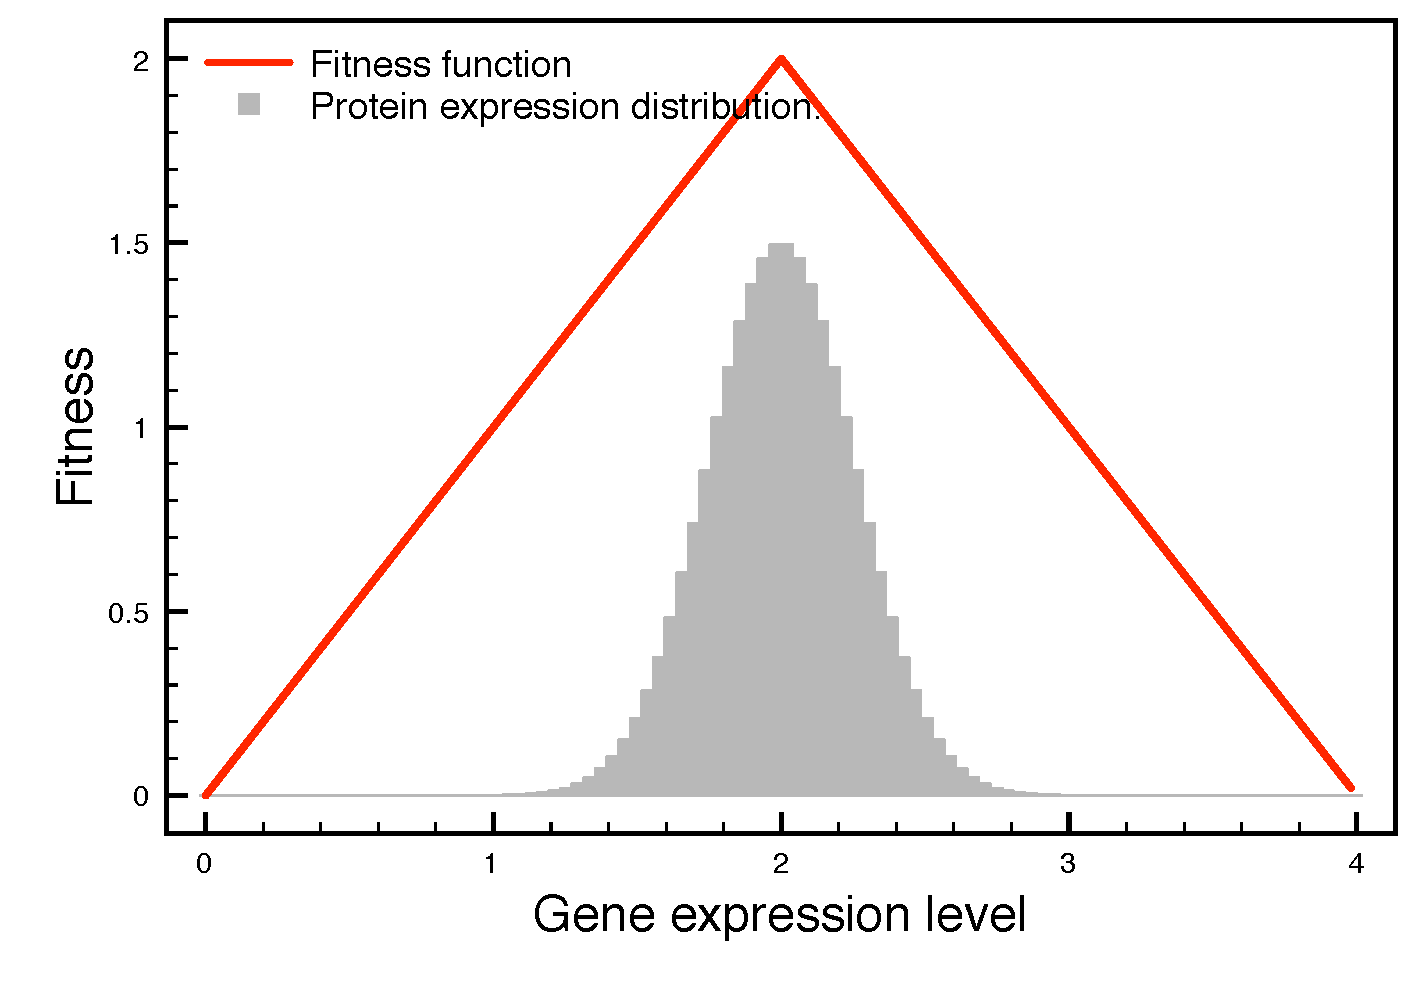
\includegraphics[width=2.5in]{triangularDistribution.pdf} &
b)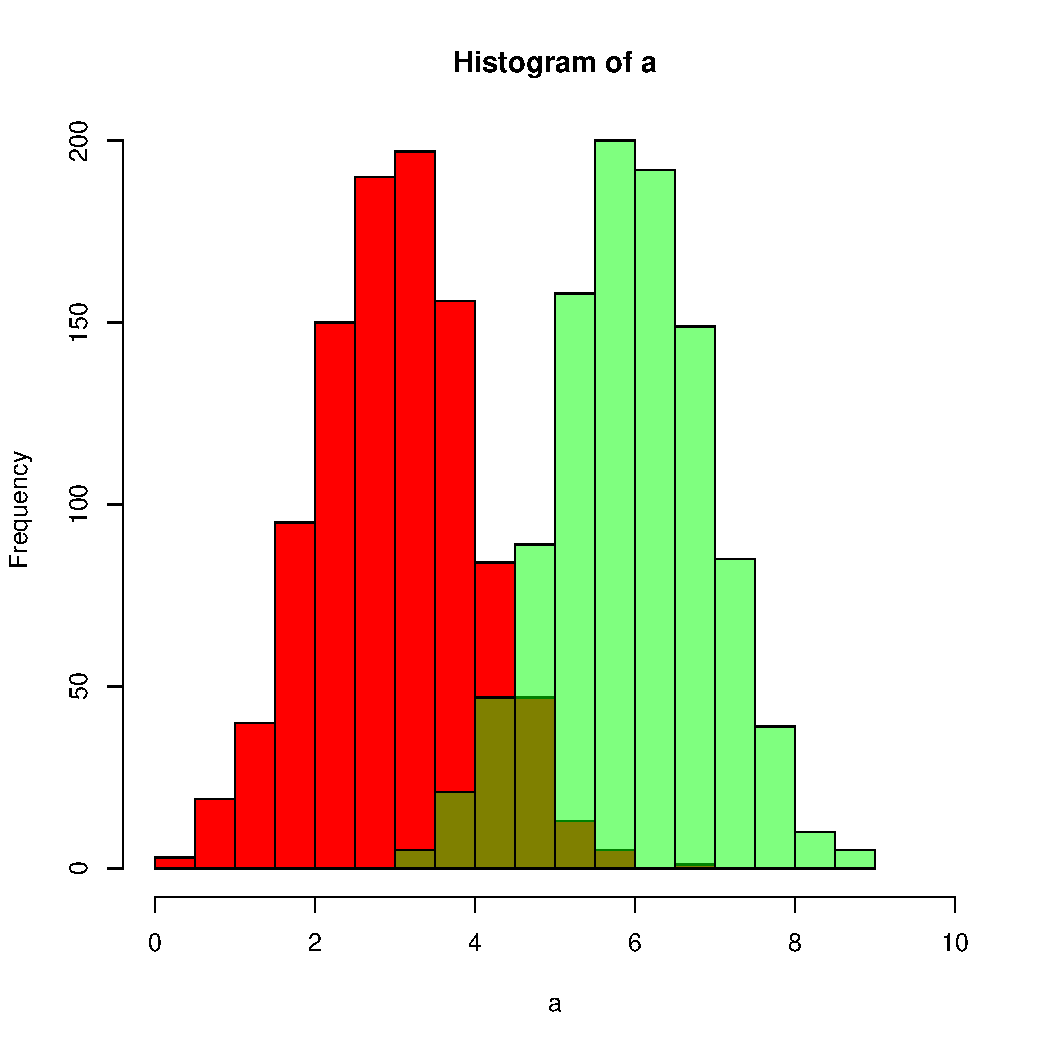
\includegraphics[width=2.5in]{Rplots.pdf}
\end{array}$
\end{center}
\caption{a): Triangular fitness function and an example of a distribution of protein expression with the form of a gaussian function. These functions are not taken from data of any biological system, they are a test tool to examine their effects on the stochastic simulation. b) In this figure is illustrated the fact that two different genes corresponding to two different phenotypes, have fitness distributions with different averages, where one phenotype is more advantageous than the other.}
\label{Fig7.2}
\end{figure}

In the next (Figure \ref{Fig7.3}) is shown the resulting fitness distribution for several  variance($\sigma$) values of the Gaussian protein distribution. 

\begin{figure}[H]
\begin{center}$
\begin{array}{cc}
a)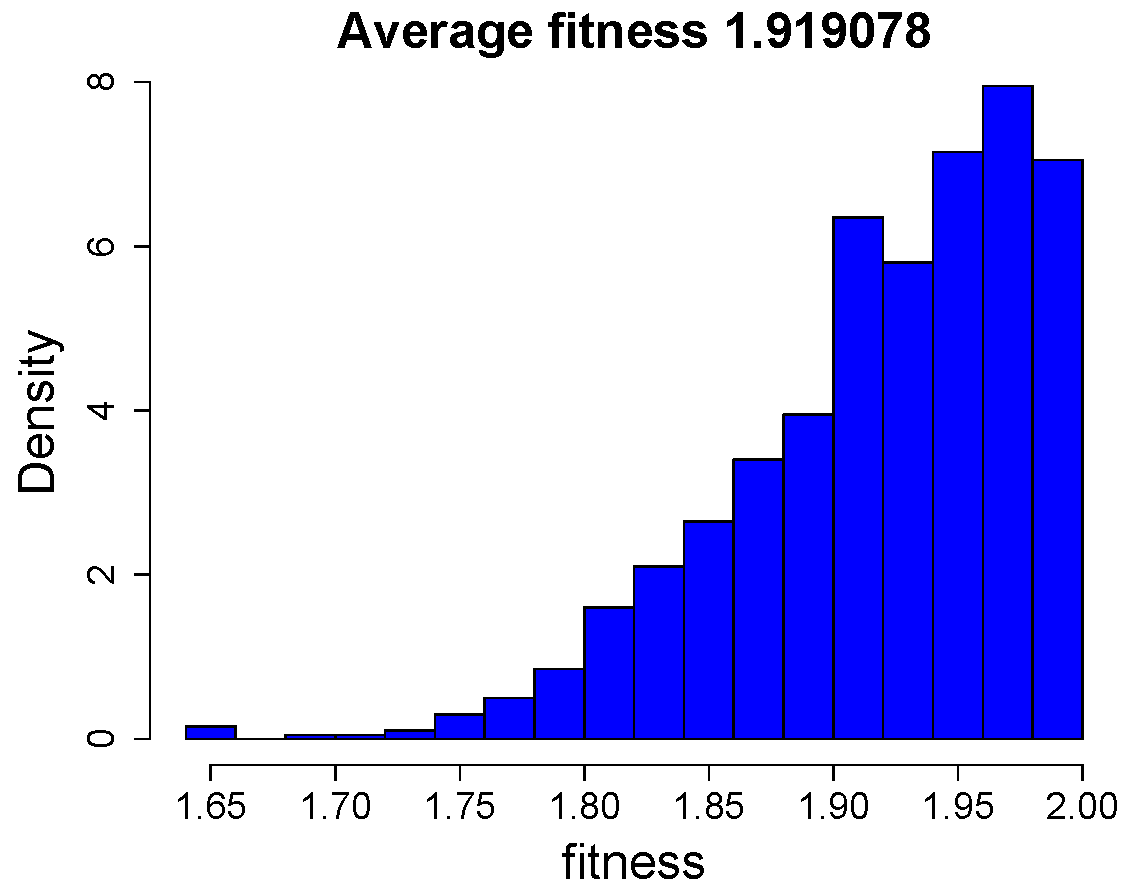
\includegraphics[width=2.5in]{triangularfitness01.pdf} &
b)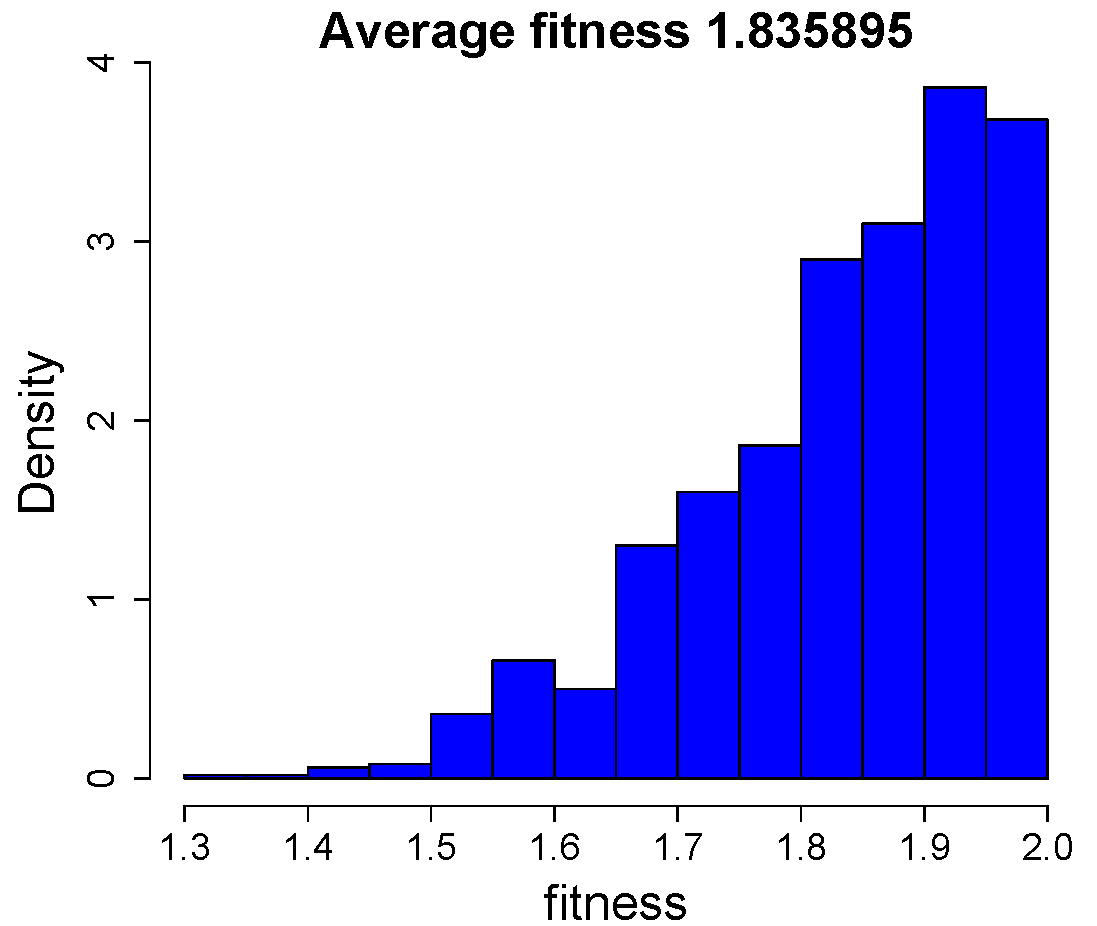
\includegraphics[width=2.5in]{triangularfitness02.pdf}\\
c)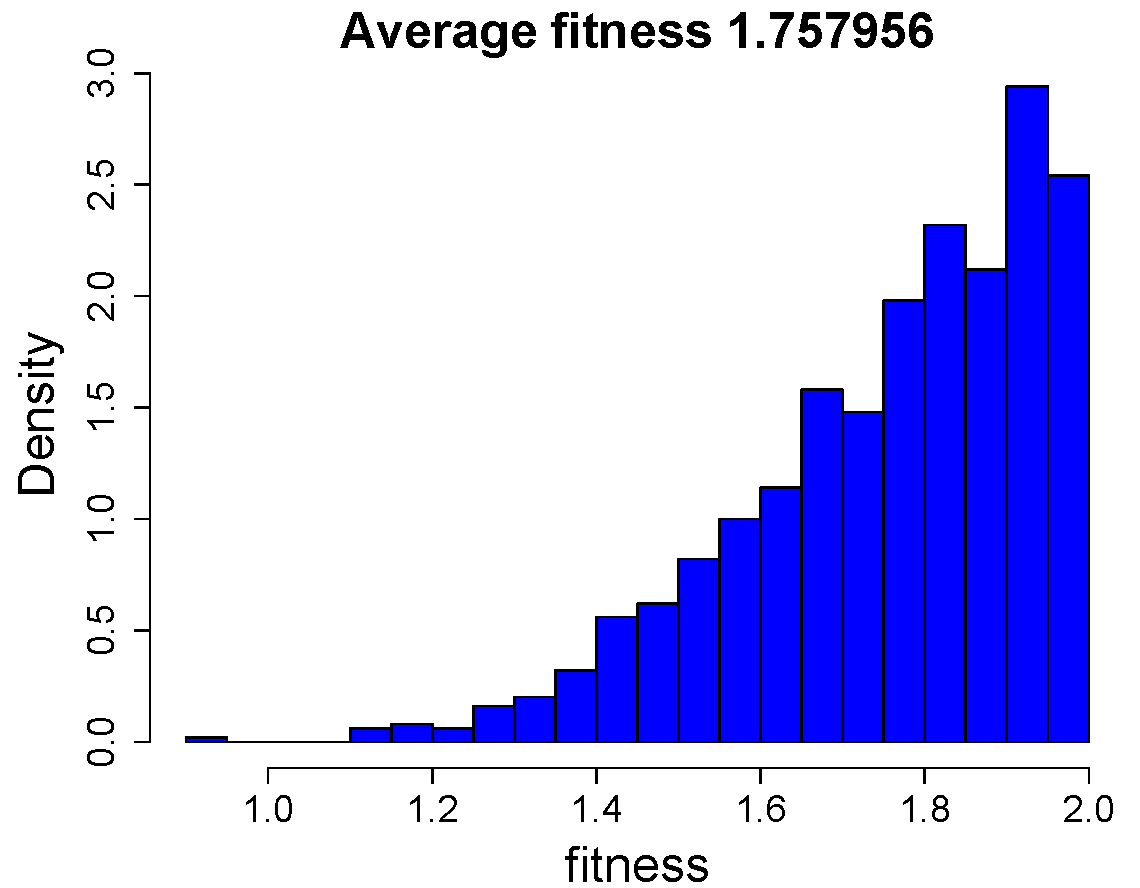
\includegraphics[width=2.5in]{triangularfitness03.pdf} &
d)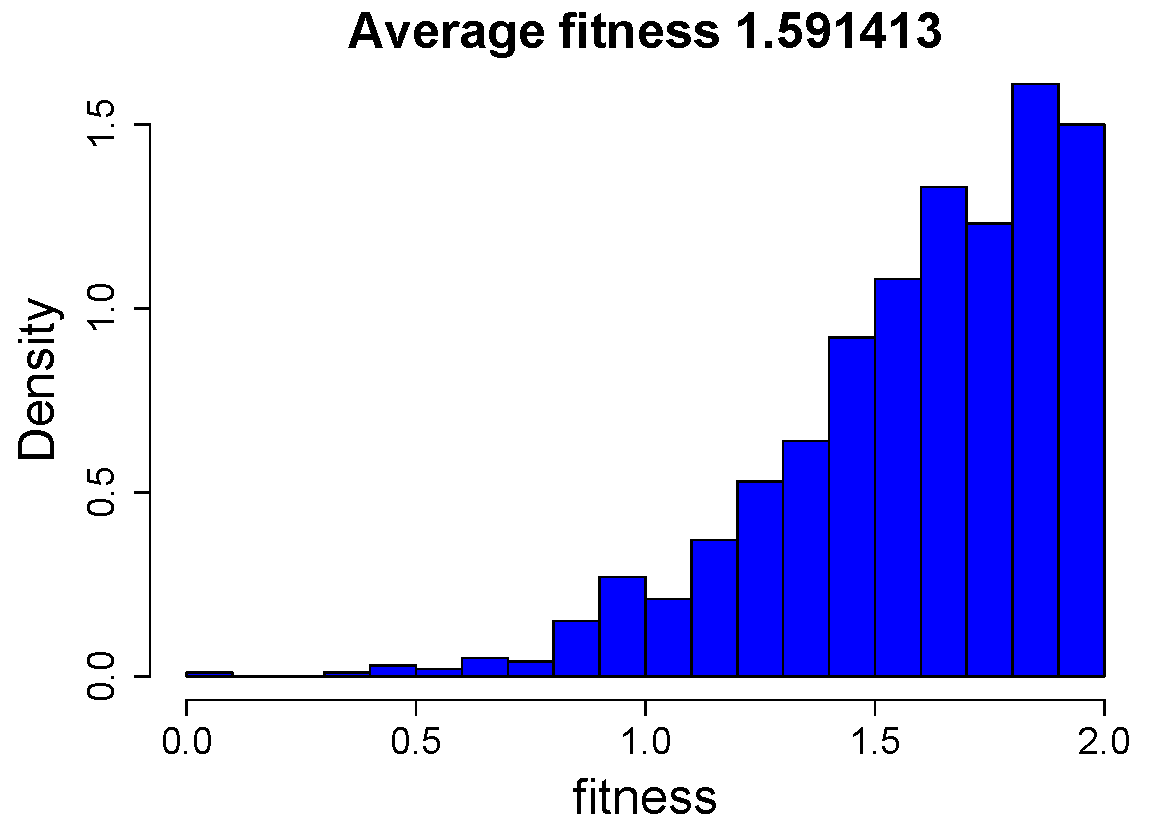
\includegraphics[width=2.5in]{triangularfitness05.pdf} 
\end{array}$
\end{center}
\caption{Fitness distributions resulting from the triangular function with optimum value $2$ and maximum fitness $2$ a) Protein expression variance $0.1$. b) Protein expression variance $0.2$. c) Protein expression variance $0.3$. d) Protein expression variance $0.5$.}
\label{Fig7.3}
\end{figure}

In (Figure \ref{Fig7.3}), is observed that average fitness decreases as variance increases. Now, the dependence of these two quantities will be examine in a graph of mean fitness versus variance $\sigma$ (Figure \ref{Fig7.4}). In this graph mean fitness has a lineal dependence with variance.
\begin{figure}[H]
  \begin{center}
    \leavevmode
    \ifpdf
      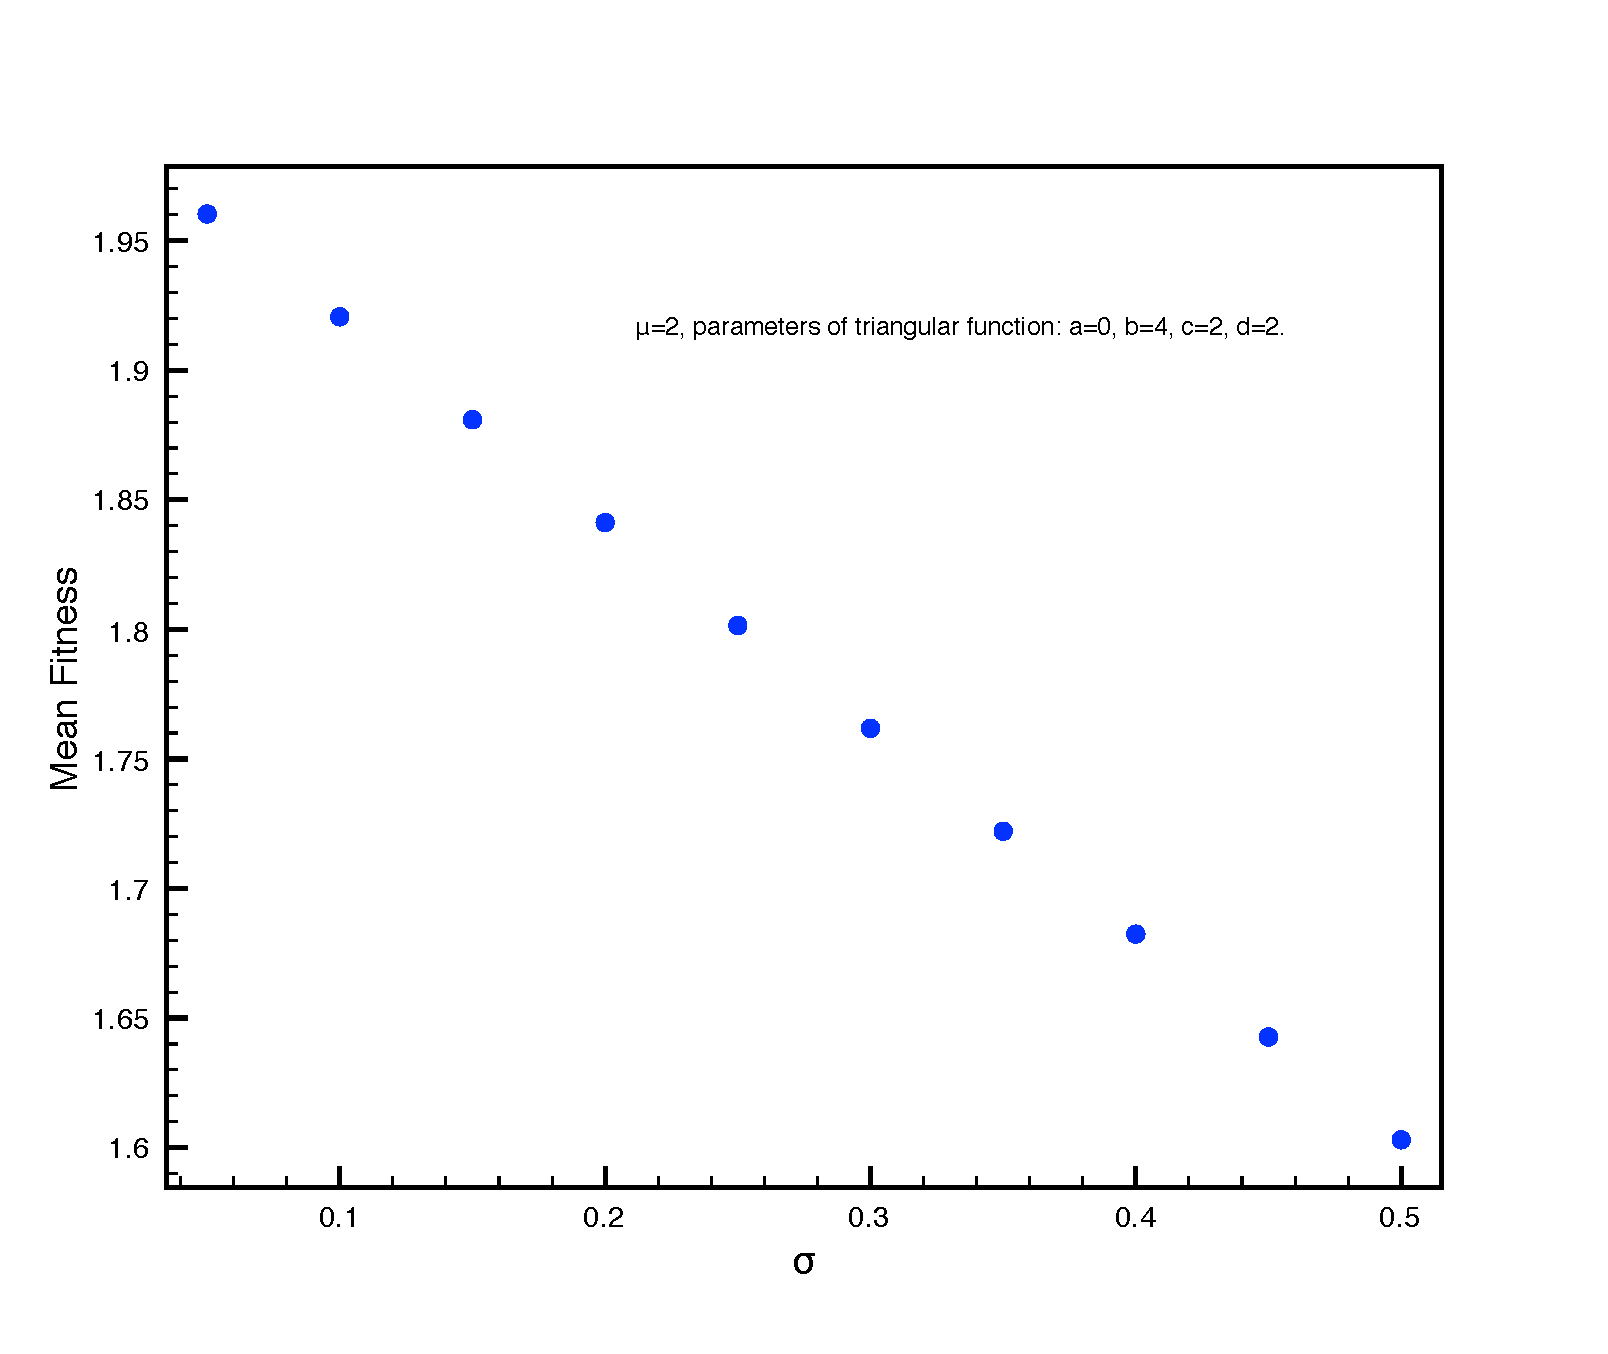
\includegraphics[width=9cm,height=8cm]{FitnessfunctionSigma.pdf}
    \else
      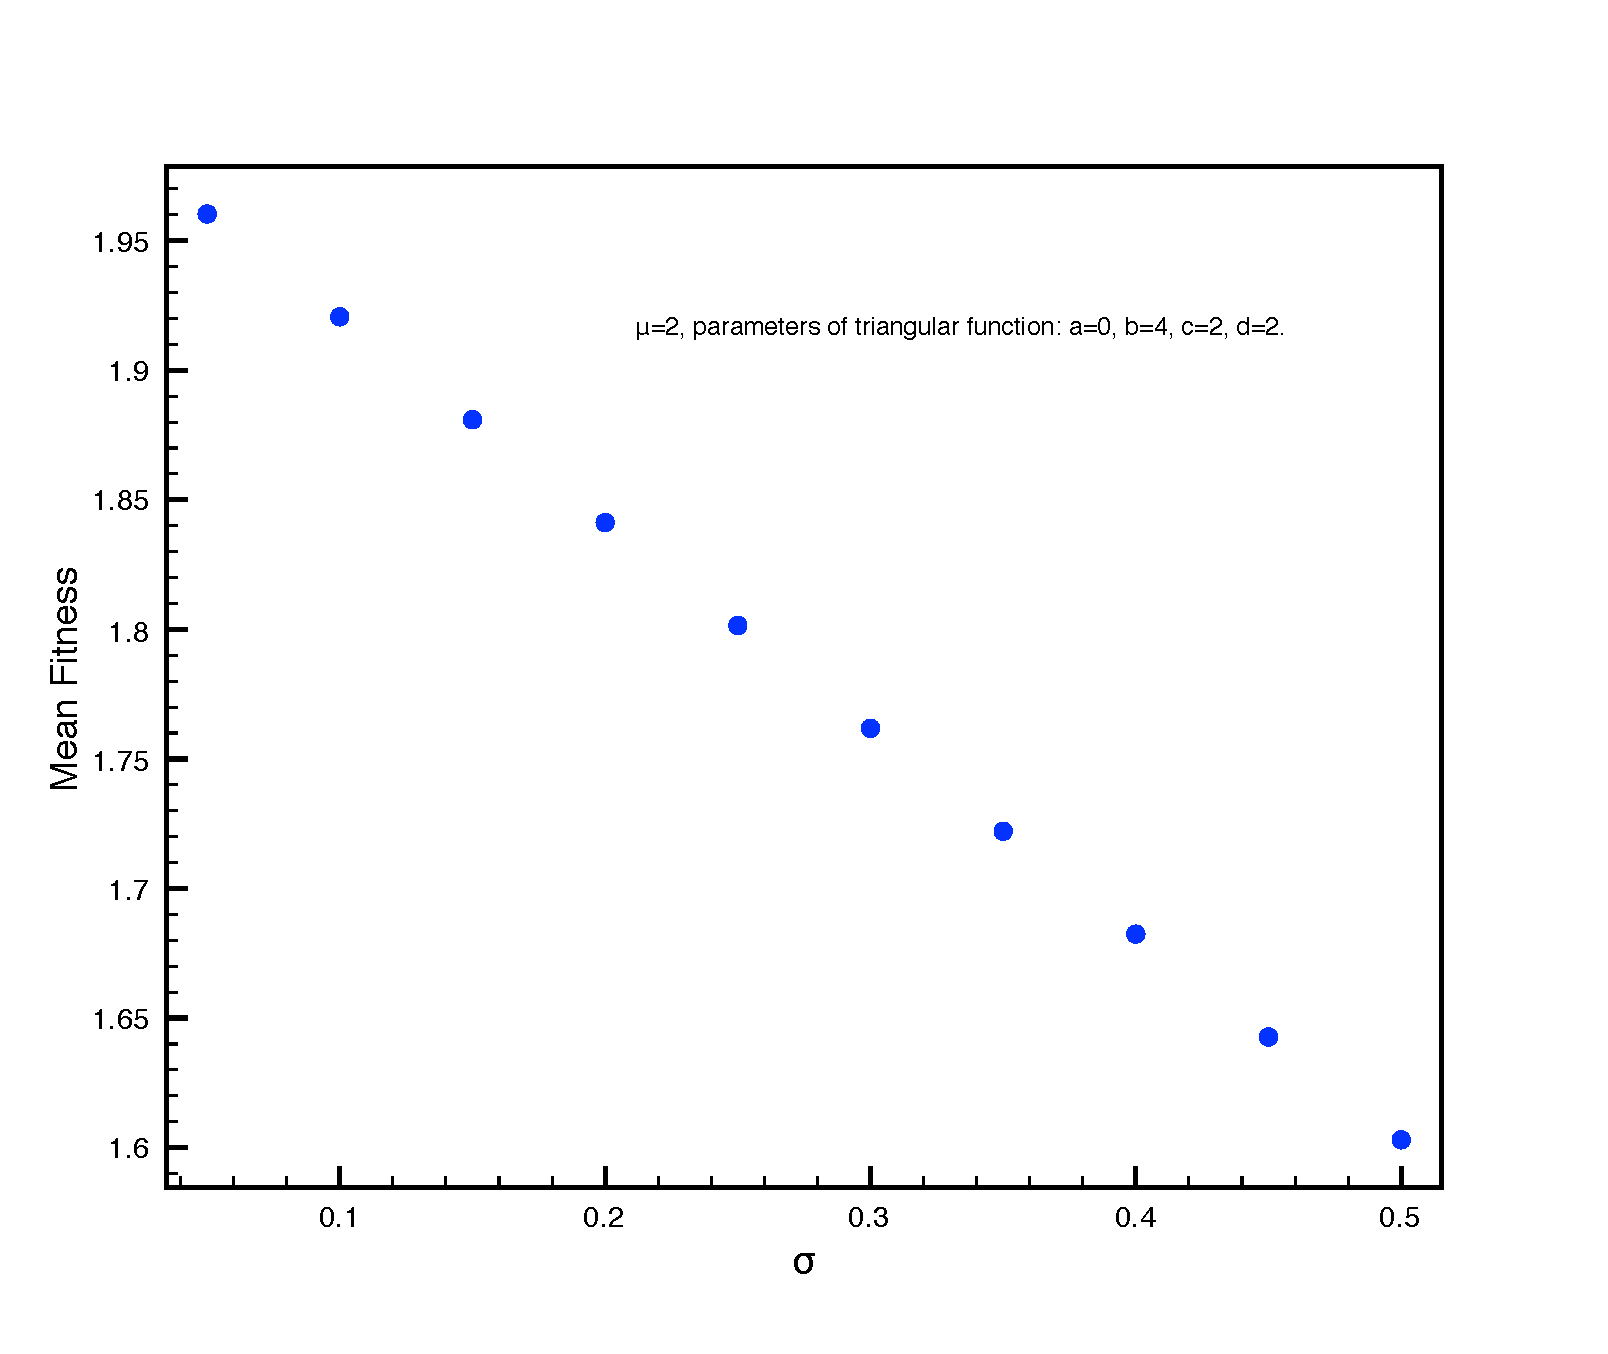
\includegraphics[width=9cm, height=8cm]{FitnessfunctionSigma.pdf}
    \fi
    \caption{Mean fitness dependence of protein variance.}
    \label{Fig7.4}
  \end{center}
  \end{figure}
The changes in  average fitness of the resulting distribution are a consequence of the non-monotonic form of fitness function. As a result, a symmetric  gaussian protein distribution generates an asymmetric fitness distribution with fitness decreasing as noise increases. Contrary, a linear increasing function have no effect on the symmetry and average of fitness as noise vary. These asymmetric resulting distributions can be classified in two types: humped toward left, and humped toward right (Figure. \ref{Fig7.4}).
\begin{figure}[H]
\begin{center}$
\begin{array}{cc}
a)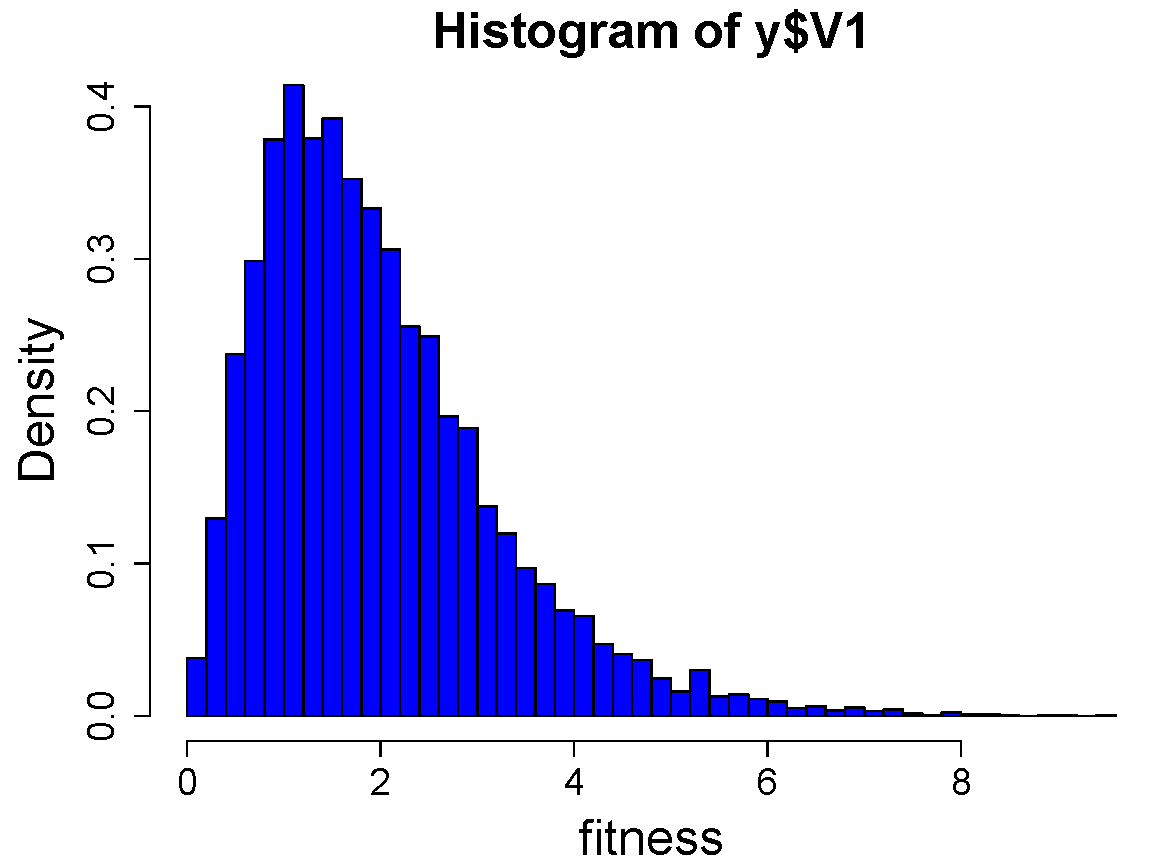
\includegraphics[width=2.5in]{humpedright.pdf} &
b)\includegraphics[width=2.5in]{humpedleft.pdf}
\end{array}$
\end{center}
\caption{a) Distribution humped toward left. These distributions characterizes because the mean is at the right hand of the mode(Gamma distribution with variance $0.3$). b) Distribution humped toward right(Extreme Value distribution with variance $0.3$). These distributions characterizes because the mean is at the left hand of the mode. The example distributions have mean equal $2$.}
\label{Fig7.4}
\end{figure}
The effects of the asymmetric shapes with growing  noise will be examine in the dynamics of moran process.

\section{Fixation Probability}
In this model model the fitness for the initial populations of individuals and their offsprings comes from a statistical distribution, which can be usually gaussian or poisson's, but for simplicity, we are initially  going to use a Gaussian distribution. Then, we will used asymmetric  distributions like gamma, to analyze the effects of symmetry in Moran process.

Let individuals of alleles of types $1$ and $0$ have values of fitness $f_{1i}$ and $f_{0j}$ respectively, that are random values from a fitness distribution. Then the probability that type $1$ is choosen for reproduction is
\begin{equation}
p_{reproduction}=\frac{\sum_{i=1}^{n}f_{1i}}{\sum_{i=1}^{n}f_{1i} + \sum_{j=1}^{N-n}f_{0j}}
\end{equation} 
where $n$ is the number of type $1$ individuals and $N$ the size of total population. Therefore the probabilities of transition are
\begin{equation}
P_{n,n+1}=\frac{\sum_{i=1}^{n}f_{1i}}{\sum_{i=1}^{n}f_{1i} + \sum_{j=1}^{N-n}f_{0j}}\frac{N-n}{N}
\end{equation}
\begin{equation}
P_{n,n-1}=\frac{\sum_{j=1}^{N-n}f_{0j}}{\sum_{i=1}^{n}f_{1i} + \sum_{j=1}^{N-n}f_{0j}}\frac{n}{N}
\end{equation}
replacing them in recursion equation
\begin{equation}
y_{n}=y_{n+1}\frac{P_{n,n+1}}{P_{n,n-1}},
\end{equation}
which leads to
\begin{equation}
y_{n}=y_{n+1}\frac{N-n}{n}\frac{\sum\limits_{i=1}^{n}f_{1i}}{ \sum\limits_{j=1}^{N-n}f_{0j}}.
\end{equation}
Since $y_1=\rho_1$, evaluating (31) for $n=1,2$ gives 
\begin{equation}
y_2 =\frac{\rho_1}{N-1}\frac{\sum\limits_{m=1}^{N-1}s_{m}}{\sum\limits_{m=1}^{1}r_{m}}
\end{equation}
\begin{equation}
y_3 =\frac{\rho_1}{N-1}\frac{\sum\limits_{m=1}^{N-1}s_{m}}{\sum\limits_{m=1}^{1}r_{m}}\frac{2}{N-2}\frac{\sum\limits_{m=1}^{N-2}s_{m}}{\sum\limits_{m=1}^{2}r_{m}}.
\end{equation}
Thus, by induction 
\begin{equation}
y_{i}=\rho_1\frac{(i-1)!(N-i)!}{(N-1)!}\prod\limits_{j=2}^{i}{\frac{\sum\limits_{m=1}^{N-(j-1)}s_m}{\sum\limits_{m=1}^{j-1}r_m}},\;\;\;\; i\geq 2.
\end{equation}
From the condition $\sum_{n=1}^{N}{y_n}=1-\rho_{1}$, the expression for $\rho_1$ is
\begin{equation}
1=\rho_1 + \sum\limits_{i=2}^{N}{\rho_1\frac{(i-1)!(N-i)!}{(N-1)!}\prod\limits_{j=2}^{i}{\frac{\sum\limits_{m=1}^{N-(j-1)}s_m}{\sum\limits_{m=1}^{j-1}r_m}}}
\end{equation}
\begin{equation}
\rho_1=\left(1 + \sum\limits_{i=2}^{N}{\frac{(i-1)!(N-i)!}{(N-1)!}\prod\limits_{j=2}^{i}{\frac{\sum\limits_{m=1}^{N-(j-1)}s_m}{\sum\limits_{m=1}^{j-1}r_m}}}\right)^{-1}
\end{equation}
For simplicity in the calculus of $\rho_{1}$ with this expression, we use $s_{m}$ as a deterministic variable. Therefore, the above equation reduces to

\begin{equation}
\rho_1=\left(1 + \sum\limits_{i=2}^{N}{(i-1)!s^{i-1}\prod\limits_{j=2}^{i}{\frac{1}{\sum\limits_{m=1}^{j-1}r_m}}}\right)^{-1}.
\end{equation}

Because $\rho_{1}$ is a function of the product among the sum of samples from a statistical distribution, $\rho_{1}$ is an stochastic variable, then we should calculated the average of $\rho_{1}$, which is the result that  simulation will give as fixation probability. The calculus of the average $\rho$ in terms of the mean and standard deviation  of the stochastic variable $r_{m}$ is really is a calculus of inferential statistics.
\section{Results}
\begin{figure}[H]
  \begin{center}
    \leavevmode
    \ifpdf
      \includegraphics[width=9cm,height=8cm]{FixationProVsNoise.pdf}
    \else
      \includegraphics[width=9cm, height=8cm]{FixationProVsNoise.pdf}
    \fi
    \caption{Fixation probability for a mutant whose type has average fitness $\bar r=2$ as a function of fitness noise from a gamma distribution, in a population of size $n=100$ and individuals of fixed fitness $s=1$.}
    \label{}
  \end{center}
  \end{figure}
  
  
\begin{figure}[H]
  \begin{center}
    \leavevmode
    \ifpdf
      \includegraphics[width=9cm,height=8cm]{AveXti700Vsnoise.pdf}
    \else
      \includegraphics[width=9cm, height=8cm]{AveXti700Vsnoise.pdf}
    \fi
    \caption{$n=100$ $s=1$ $i=1$ gamma average $2$ Time $700$.}
    \label{}
  \end{center}
  \end{figure}
  
  \begin{figure}[H]
  \begin{center}
    \leavevmode
    \ifpdf
      \includegraphics[width=9cm,height=8cm]{Averagefixationtimervariance1001.pdf}
    \else
      \includegraphics[width=9cm, height=8cm]{Averagefixationtimervariance1001.pdf}
    \fi
    \caption{$n=100$ $s=1$ $i=1$ gamma $r$ average $2$ .}
    \label{}
  \end{center}
  \end{figure}
  
  Fitness function of protein expression
\begin{figure}[H]
\begin{center}$
\begin{array}{cc}
a)\includegraphics[width=2.5in]{exremeValueFixation.pdf} &
b)\includegraphics[width=2.5in]{histextremevalue.pdf}
\end{array}$
\end{center}
\caption{a): Fixation probability for increasing variance of a extreme value distribution, where $n=100$, $\bar{r}=1$, $s=0.7$ and initial population $i=1$. b) Extreme value distribution used in simulation for variance $0.001$. This distribution is humped toward right .}
\label{Fig7.2}
\end{figure}
Time fixation as a function of noise in protein level

  
\begin{figure}[H]
\begin{center}$
\begin{array}{cc}
a)\includegraphics[width=2.5in]{TriangularFunction.jpg} &
b)\includegraphics[width=2.5in]{triangularfunctionHistogram.pdf}
\end{array}$
\end{center}
\caption{a): Fitness triangular function of expression level. b): Resulting fitness distribution due to triangular function.}
\label{Fig7.2}
\end{figure}
Time fixation as a function of noise in protein level

  \begin{figure}[H]
\begin{center}$
\begin{array}{cc}
a) \includegraphics[width=2.5in]{SigmaVariationLTfitness.pdf} &
b)\includegraphics[width=2.5in]{nocenteredVsSigma.pdf}
\end{array}$
\end{center}
\caption{a): Average time when $10$ initial mutants(mean fitness=2) reach  $50\%$ of the population. This graph shows the average  time using a gaussian distribution with a linear function and with a non-linear function centered with the gaussian distribution. b): Average fixation time when the expression distribution is not centered with the fitness function. Fitness function centered on $10$ and distribution centered on $11$ and $12$.}
\label{Fig7.3}
\end{figure}
Really it is a function of average fitness of the distribution resulting from the fitness protein function.

\begin{figure}[H]
\begin{center}$
\begin{array}{cc}
a)\includegraphics[width=2.5in]{FitnessfunctionSigma.pdf} &
b)\includegraphics[width=2.7in]{AveragetimeFitness.pdf}
\end{array}$
\end{center}
\caption{a): Average resulting fitness from the triangular function as a function as the noise expression level. b): Average fixation time as a function of the mean fitness.}
\label{Fig7.4}
\end{figure}
See the average population fitness in time.
\section{The Fluctuation-Dissipation Theorem}
The fluctuation dissipation theorem is an approach to noise between different species in a stochastic system of coupled reactions. This theorem is based on the $\Omega$ expansion around to the stable points in  master equation\cite{Kampen}, which leads to a system of time differential equations for the variances of  different species in the stochastic system. The matrix formulation of this theorem is as follow\cite{Paulsson2005}  
\begin{equation}
\frac{d\boldsymbol{\sigma}}{dt}=\mathbf{A}\boldsymbol{\sigma} + \boldsymbol{\sigma}\mathbf{A}^{T} + \mathbf{B}
\end{equation}
where $\sigma_{ij}$ are the covariances and
\begin{equation}
A_{ij}=\frac{\partial}{\partial \langle n_j \rangle}\frac{\partial\langle n_i\rangle}{\partial t}\;\; ,\;\; B_{ij}=\sum\limits_{k}v_{jk}v_{ik}R_{k}
\end{equation}
$n_{i}$ are the quantities involved in the stochastic process. $B_{ii}$ is the sum of fluxes for each species $n_{i}$. When there are no equation for terms of the form$\partial_t\langle n_i n_j\rangle$, which represent events that change two different species simultaneously, $B_{ij}=0$\cite{Paulsson2005}. 

As an example to learn how  this theorem works, we can solve these equations in a system of protein synthesis from mRNA, where the average number of proteins is denoted by $\langle x\rangle$ and the mRNA by $\langle y\rangle$. They follow the dynamics.
\begin{equation}
\partial_{t}\langle y\rangle=\lambda_{1}- \beta_{1}\langle y\rangle
\end{equation}  
\begin{equation}
\partial_{t}\langle x \rangle=\lambda_{2}\langle y\rangle - \beta_{2}\langle x\rangle
\end{equation}
thus
\begin{equation}
\mathbf{A}=
\begin{pmatrix}
-\beta_1 & 0 \\
\lambda_2 & -\beta_2
\end{pmatrix}\;\; , \;\; \mathbf{B}=\begin{pmatrix} \lambda_1 + \beta_1 \langle y\rangle & 0 \\
0 & \lambda_2\langle y\rangle+ \beta_2\langle x\rangle\end{pmatrix}
\end{equation}
Finally the matrix for time derivates of variances is
\begin{equation}
\begin{pmatrix} \partial_{t} \sigma_{y}^{2} & \partial_t \sigma_{xy}\\
\partial_t \sigma_{xy} & \partial_t \sigma_{x}^{2}
\end{pmatrix}
=
\begin{pmatrix} -2\sigma_{yy}\beta_{1}+\beta_1\langle y\rangle+\lambda_1 & \lambda_2\sigma_{yy}-\sigma_{yx}\beta_2-\beta_1\sigma_{xy}\\
\lambda_2\sigma_{yy}-\sigma_{yx}\beta_2-\beta_1\sigma_{xy} & \lambda_2\langle y\rangle-\beta_2 \langle x\rangle + 2(\lambda_2\sigma_{xy}-\beta_2\sigma_{xx})
\end{pmatrix}
\end{equation}
Thus the respective differential equations for each variance are

\begin{gather}
\frac{d \sigma_{y}^{2}}{dt}=-2\sigma_{yy}\beta_1 + \beta_1 \langle y\rangle + \lambda_1\;\;, \;\; \frac{d\sigma_{xy}}{dt}= \lambda_2\sigma_{yy}-\sigma_{yx}\beta_2-\beta_1\sigma_{xy} \notag \\
\frac{d\sigma_{x}^{2}}{dt}=\lambda_2\langle y\rangle-\beta_2 \langle x\rangle + 2(\lambda_2\sigma_{xy}-\beta_2\sigma_{xx})
\end{gather}
In steady state the noise $\eta_{x}^{2}=\sigma_{x}^{2}/\langle x\rangle^2$ for proteins is related with mRNA noise $\eta_{y}^{2}=1/\langle y\rangle$ by the equation
\begin{equation}
\eta_{x}^{2}=\frac{1}{\langle x\rangle} +\frac{1}{\langle y\rangle(1+\beta_1/\beta_2)}.
\end{equation} 
In this equation we can see the intrinsic poissonian noise $1/\langle x\rangle$ and the external noise; the second term, which is the mRNA poissonian noise scaled by factor that depends on the degradation rates. This noise relation can also be  derived using the moment generating function\cite{Pedraza1}.
\section{Fluctuation-Dissipation Theorem for Random Drift and Stochastic Fitness}
In random drift two types of organisms with fitnesses $r$ and $s$ compete in population of fixed size $n$. In this system, the population fraction $\langle x\rangle$ of individuals with fitness $r$  follow sthe time differential equation
\begin{equation}
\frac{d \langle x\rangle}{dt}=\frac{r\langle x\rangle(1-\langle x\rangle)}{n(r\langle x\rangle + s(1-\langle x\rangle))}-\frac{s\langle x\rangle(1-\langle x\rangle)}{n(r\langle x\rangle + s(1-\langle x\rangle))},
\end{equation} 
where for simplicity we are going to use $\langle x\rangle=\bar{x}$.

The first two derivatives respect to $\bar{x}$ for the probability fluxes of this equation are:
\begin{equation}
\frac{\partial}{\partial\bar{x}}\frac{d\bar{x}}{dt}=\frac{r-s}{n}\left[\frac{(1-2\bar{x})(r\bar{x}+s(1-\bar{x}))-\bar{x}(1-\bar{x})(r-s)}{\left(r\bar{x}+s(1-\bar{x})\right)^{2}}\right]
\end{equation} 
\begin{equation}
\frac{\partial^{2}}{\partial\bar{x}^{2}}\frac{d\bar{x}}{dt}=\left[\frac{(2\bar{x}(s-r)-2s)(r\bar{x}+s(1-\bar{x}))-2(r-s)(s-\bar{x}^{2}(r-s)-2\bar{x}s)}{\left(r\bar{x}+s(1-\bar{x})\right)^{3}}\right]
\end{equation}
Thus the differential equation for $\sigma_{xx}$ in the case of fixed fitness is
\begin{equation}\label{7.22}
\frac{d\sigma_{xx}}{dt}=2\sigma_{xx}\frac{r-s}{n^2}\left[\frac{(1-2\bar{x})(r\bar{x}+s(1-\bar{x}))-\bar{x}(1-\bar{x})(r-s)}{\left(r\bar{x}+s(1-\bar{x})\right)^{2}}\right] + \frac{\bar{x}}{n^{2}}\frac{(1-\bar{x})(r+s)}{r\bar{x}+s(1-\bar{x})},
\end{equation}
where the general equation for $\sigma_{ij}$ has been divided by $n$ because generally in literature the time step $dt$ is rescale to $dt/n$. This was done to have compatibility with simulations, where time is not rescale to  size $n$ of the system. In the next (Figure \ref{Fig7.5}), the solution of Eq. \eqref{7.22} is plotted with different simulations for random drift with deterministic fitness and noise fitness. It is observed that the variance differential equations has  maximum value at similar times in the simulation.  
\begin{figure}[H]
  \begin{center}
    \leavevmode
    \ifpdf
      \includegraphics[width=9cm,height=8cm]{VarianceNoiseNonoiseAnalytical.pdf}
    \else
      \includegraphics[width=9cm, height=8cm]{VarianceNoiseNonoiseAnalytical.pdf}
    \fi
    \caption{In this graph there are several plots for  noise $\eta_{x}^{2}=\sigma_{xx}/\langle x\rangle^2$. There are curves from the stochastic simulation and one, that is the solution of the analytical differential equation for variance. In the simulations for random drift $\bar{r}=2$, $s=1$ and the noise for $r$ is $0.4$(gaussian distribution), $n=1000$ and $i=10$. The simulation data were obtained with $1000$ simulations, which is not an enough large to have similar curves in each execution of the program.}
    \label{Fig7.5}
  \end{center}
  \end{figure}

\begin{figure}[H]
  \begin{center}
    \leavevmode
    \ifpdf
      \includegraphics[width=9cm,height=8cm]{noisepopulation100.pdf}
    \else
      \includegraphics[width=9cm, height=8cm]{noisepopulation100.pdf}
    \fi
    \caption{In this graph there are several plots for  noise $\eta_{x}^{2}=\sigma_{xx}/\langle x\rangle^2$. In the simulations for random drift $\bar{r}=2$, $s=1$, and the random values for $r$ come from a gamma distribution with different variance for each curve. The population size is $n=100$ and the initial number of individual with fitness $r$ is  $i=1$. The simulation data were obtained with $10^4$ simulations.}
    \label{}
  \end{center}
  \end{figure}

\begin{figure}[H]
  \begin{center}
    \leavevmode
    \ifpdf
      \includegraphics[width=9cm,height=8cm]{noise10010gammavariance.pdf}
    \else
      \includegraphics[width=9cm, height=8cm]{noise10010gammavariance.pdf}
    \fi
    \caption{In this graph there are several plots for  noise $\eta_{x}^{2}=\sigma_{xx}/\langle x\rangle^2$. In the simulations for random drift $\bar{r}=2$, $s=1$, and the random values for $r$ come from a gamma distribution with different variance for each curve. The population size is $n=100$ and the initial number of individual with fitness $r$ is  $i=10$. The simulation data were obtained with $10^4$ simulations.}
    \label{}
  \end{center}
  \end{figure}
  
\begin{figure}[H]
\begin{center}$
\begin{array}{cc}
a)\includegraphics[width=2.5in]{VarianceTime10001noise.pdf} &
b)\includegraphics[width=2.7in]{AverageTime10001noise.pdf}
\end{array}$
\end{center}
\caption{In this graph there are several plots for  noise $\eta_{x}^{2}=\sigma_{xx}/\langle x\rangle^2$. In the simulations for random drift $\bar{r}=2$, $s=1$, and the random values for $r$ come from a gamma distribution with different variance for each curve. The population size is $n=1000$ and the initial number of individual with fitness $r$ is  $i=1$. The simulation data were obtained with $10^4$ simulations.a) Standard deviation curves. b) Average population fraction curves. It can be observed that the standard deviations and the difference in the population average are smaller than the case for $n=100$, which means that for large populations the effects of internal noise decrease.}
\label{}
\end{figure}



In this system of natural selection, fitness is not a deterministic variable, which affects the birth and death fluxes for $\bar{ x}$. Fitness depends on the protein expression  of each cell or individual.  The average equation for protein expression $\bar{p}$ 
\begin{equation}
	\frac{d \bar{p}}{dt}=\beta(\bar{y}_{1}, ...., \bar{y}_{k}) - \lambda \bar{p}.
\end{equation} 
Where $\beta(\bar{y}_{1}, ...., \bar{y}_{k})$ is a function of the $k$ reactions in the genetic network. We can consider the case where phenotypic proteins are not altered by the rest of metabolic network. 

For simplicity $s$ will be considered deterministic and $r(p)$ stochastic. 

Then, the matrices $\mathbf{A}$ and $\mathbf{B}$ for this system are

\begin{equation}
\begin{split}
\mathbf{A}&=\begin{pmatrix} -\lambda & 0 \\
\partial_{p}\frac{d\bar{x}}{dt} & \partial_{\bar{x}}\frac{d\bar{ x}}{dt}
\end{pmatrix}\;\; , \\ \mathbf{B}&=\begin{pmatrix}\beta(\bar{y}_{1}, ...., \bar{y}_{k}) + \lambda\bar{p} & 0 \\
0 & \frac{\bar{x}(1-\bar{x})}{n(r(\bar{p} )\bar{x}+ s(1-\bar{x}))}(r(\bar{p})+ s)
\end{pmatrix}
\end{split}
\end{equation}
Therefore the variance equations are
\begin{gather}
\frac{d\sigma_{pp}}{dt}=-2\lambda\sigma_{pp}+\beta(\bar{y}_{1}, ...., \bar{y}_{k})+ \lambda\bar{p} \;\; , \;\; \frac{d\sigma_{px}}{dt}=\sigma_{pp}\partial_{\bar{ p}}\frac{d\bar{ x}}{dt} + \sigma_{xp}\partial_{\bar{x}}\frac{d\bar{x}}{dt} - \lambda\sigma_{xp} \notag \\
\frac{d\sigma_{xx}}{dt}=2\left(\partial_{\bar{p}}\frac{d\bar{x }}{dt} \sigma_{xp} + \sigma_{xx}\partial_{\bar{x}}\frac{d\bar{ x}}{dt} \right) + \frac{\bar{x}(1-\bar{x})}{n(r(\bar{p})\bar{x}+ s(1-\bar{x}))}(r(\bar{p})+ s)
\end{gather}
We are interested in the direct relation of fitness variability with population dynamics. To examine this, we can considerate that for each generation of cells(a birth and death event), all of them would have reached its internal steady state, which is valid  because of the large difference between the times for protein events and a birth and death cell. Hence $\sigma_{pp}$ is a time constant respect to the Moran process.
\begin{equation}
0=-2\lambda\sigma_{pp}+\beta(\bar{y}_{1}, ...., \bar{y}_{k})+ \lambda\bar{p} 
\end{equation} 
 

%%% ----------------------------------------------------------------------

%%% Local Variables: 
%%% mode: latex
%%% TeX-master: "../thesis"
%%% End: 

%%% Thesis Introduction --------------------------------------------------
\chapter{Stochastic Cooperation}
\ifpdf
    \graphicspath{{StochasticCooperation/Figs/PNG/}{StochasticCooperation/Figs/PDF/}{StochasticCooperation/Figs/}}
\else
    \graphicspath{{StochasticCooperation/Figs/EPS/}{StochasticCooperation/Figs/}}
\fi
To simulate stochastic cooperation we use a more simple game where there are not pair interaction among individuals, this game is a system of common goods, where individuals in a group interact through a common source of any benefit.  This describes a classic game in behavioral economics\cite{Szabo2002} where a  group of people is given an amount of money, each person has to contribute money, and the total amount is divided by the number of people in the group, and then each individual gets back this quantity times a factor larger than one.

 In this model  each individual invests a random cost $c_{i}$, and everyone obtains a common benefit $b=B\frac{\sum c_{i}}{n}$, where the benefit factor $B\geqslant1$ . The utility of each individual is $u_{i}=b-c_{i}$. Therefore, if everyone cooperates with the same amount they get back a larger amount, but if just some individuals cooperate, they will get back a smaller amount than invested. Furthermore, if nobody cooperate, there will be not payoff. 
 
 The expected payoff of a cooperator is
   \begin{equation}
   \pi_{C}=\frac{\sum_{j=1}^{i}b-c_{cj}}{i}
   \end{equation}   
   and the fitness is
   \begin{equation}
   f_{c}=1-w+w\pi_{c}
   \end{equation} 
   In our simulations we used $w=1$.

 
    In a bacterial example, plasmids in E.coli are the individuals and the E.coli are the groups. The plasmids take nutrients from the cell for their own reproduction, but when they take too much the bacteria will reproduce slower. 
    Another example is when a group of bacteria produce  an enzyme to process a food source, which all the bacteria have equal accessibility.  
    
    
  We used this cooperation model to simulate group selection in individuals with no deterministic degree  of cooperation. The population was divided in two types, where their cooperation degrees come from Gaussian distributions with different means and standard deviations. Different measures of fixation probability as a function of noise and benefit were done for this system, as shown bellow.   
 \begin{figure}[H]
\begin{center}$
\begin{array}{cc}
a)\includegraphics[width=2.5in]{fixprobabilityVsBenefit.pdf} &
b)\includegraphics[width=2.7in]{fixprobabilityVsmean1Benefit.pdf}
\end{array}$
\end{center}
\caption{a): Fixation probability as a function of benefit when initially all groups are homogeneous . b): Fixation probability as a function of mean cost for several values of benefit.}
\label{Fig8.1}
\end{figure}

\begin{figure}[H]
\begin{center}$
\begin{array}{cc}
a)\includegraphics[width=2.5in]{fixprobabilityVsmean0.pdf} &
b)\includegraphics[width=2.7in]{fixprobabilityVsmean1Sigmas.pdf}
\end{array}$
\end{center}
\caption{a): Fixation probability of cooperators as a function of mean degree of defectors cooperation. b): Fixation probability of cooperators as a function of their mean degree cost. The graph shows different points for several values of benefit when all the groups are initially homogeneous.}
\label{Fig8.2}
\end{figure}
It  is seen that initially for a group where there is a defector, this individual have a larger probability of reproduction than the rest of the group, but as this kind of individuals reproduce, the overall fitness of the group decreases respect to the rest of the groups with cooperators.
\begin{figure}[H]
\begin{center}$
\begin{array}{cc}
a)\includegraphics[width=2.5in]{probaCoopeSinglegroup.pdf} &
b)\includegraphics[width=2.7in]{probaCoomixedGroup.pdf}
\end{array}$
\end{center}
\caption{a): Fixation probability of $50$ cooperators in a group of size $100$. b): Fixation probability when a population of $m=10$ and $n=10$ has initially a mixed group with $5$ cooperators and the rest of the groups are deffectors.}
\label{Fig8.3}
\end{figure}

%%% ----------------------------------------------------------------------

%%% Local Variables: 
%%% mode: latex
%%% TeX-master: "../thesis"
%%% End: 

\def\baselinestretch{1}
\chapter{Conclusions}
\ifpdf
    \graphicspath{{Conclusions/ConclusionsFigs/PNG/}{Conclusions/ConclusionsFigs/PDF/}{Conclusions/ConclusionsFigs/}}
\else
    \graphicspath{{Conclusions/ConclusionsFigs/EPS/}{Conclusions/ConclusionsFigs/}}
\fi

\def\baselinestretch{1.66}


 \begin{itemize}
             \item The mean time of fixation is not affected if fitness is a linear function of protein expression, and protein distribution is symetric.
             \item The mean fixation time is affected when the fitness is not a linear function of protein expression, and it is longer when genetic noise is larger. But if we see the distribution fitness that result from the fitness function, the mean fitness determines the average time fixation. This means that the fitness standard deviation dose not affect.
             \item  In group selection when all the initial groups are homogeneous, the fixation of probability dose not depend on the benefit(Figure 15), but as it is seen in (Figure 17) when there is an initial mixed group fixation probability is affected by benefit. 
             \item  In (Figure16) is observed the first level of cooperation, where cooperator are fitter as the benefit increase. From Figures (16 and 17) is observed that the two levels of selection have different behavior  as a function of benefit.   
             \item Propose   a new way for simulate group selection and the dilemma of cooperate or defect. Where the benefit of cheating can be seen more clearly.     
             \item Fitness noise have considerable effects on the fixation probabilities in random drift when fitness distribution is asymmetric, as gamma distribution, where was observed that fixation probability decreased as  fitness variance increased.  For gaussian distributions the effects of noise are too small to be considered. Furthermore, depending on the symmetry  of fitness distribution, noise can favor fixation probability, if this is such that most of individuals have a fitness larger than the average of the distribution. 
              \end{itemize}

Cosas por hacer : graficas de $\sigma^{2}$ vs $t$, Resolver ecuacion de $\sigma_{xx}, \sigma_{pp}$, $\rho_{i}$ $T_{i}$ analitico estocastico.
%%% ----------------------------------------------------------------------

% ------------------------------------------------------------------------

%%% Local Variables: 
%%% mode: latex
%%% TeX-master: "../thesis"
%%% End: 


\backmatter % book mode only
\appendix
\chapter{Appdx A}

and here I put a bit of postamble ...

% ------------------------------------------------------------------------

%%% Local Variables: 
%%% mode: latex
%%% TeX-master: "../thesis"
%%% End: 

\chapter{Appdx B}

and here I put some more postamble ...

% ------------------------------------------------------------------------

%%% Local Variables: 
%%% mode: latex
%%% TeX-master: "../thesis"
%%% End: 


\bibliographystyle{plain}
%\bibliographystyle{Classes/CUEDbiblio}
%\bibliographystyle{Classes/jmb}
%\bibliographystyle{Classes/jmb} % bibliography style
\renewcommand{\bibname}{References} % changes default name Bibliography to References
\bibliography{References/references} % References file

\end{document}
